\documentclass[a4paper,twoside]{article}

\usepackage[utf8]{inputenc}
\usepackage[italian]{babel}
\usepackage{amsmath,amsthm}
\usepackage{amssymb,amsfonts}
\usepackage{dsfont}
\usepackage{graphicx}
\usepackage[obeyspaces]{url}
\usepackage[colorlinks = true,
            linkcolor = blue,
            urlcolor  = blue,
            citecolor = blue,
            anchorcolor = blue]{hyperref}
\usepackage{color}
\usepackage{xcolor}
\usepackage{enumitem}
\usepackage{framed}
\usepackage{skull}
\usepackage{stackengine}
\usepackage{scalerel}
\usepackage{mathrsfs}
\usepackage{wasysym}
\usepackage{tikz}
\usepackage{relsize}
\usepackage{cancel}
\usepackage{fontawesome}
\usepackage[font=small]{caption}
\colorlet{shadecolor}{blue!9}
\definecolor{Red}{rgb}{0,0,0.3}

\setlength{\headheight}{14pt}
\setlength{\topmargin}{-1cm}
\setlength{\evensidemargin}{-1cm}
\setlength{\oddsidemargin}{-1cm}
\setlength{\textwidth}{18cm} 
\setlength{\textheight}{25cm}

\linespread{1.2}

\usepackage{lastpage}

\usepackage{fancyhdr}
\pagestyle{fancy}
\fancyhead{} % clear all header fields
\fancyhead[RE]{\slshape \rightmark}
\fancyhead[LO]{\slshape \leftmark}
%\fancyhead[CO,CE]{\bfseries Jacopo D'Aurizio - Esercizi svolti di Analisi 1}
\fancyfoot{} % clear all footer fields
\fancyfoot[CE,CO]{Pagina \thepage\ / \pageref{LastPage}}
\renewcommand{\headrulewidth}{0.4pt}
\renewcommand{\footrulewidth}{0.2pt}
\renewcommand{\epsilon}{\varepsilon}

%\renewcommand{\thesubsection}{\Roman{subsection}}
\newcommand{\mydef}{\;\dot{=}_{\!\!\!\!\mbox{. }}}
\newcommand{\N}{\mathbb{N}}
\newcommand{\Z}{\mathbb{Z}}
\newcommand{\Q}{\mathbb{Q}}
\newcommand{\C}{\mathbb{C}}
\newcommand{\R}{\mathbb{R}}
\newcommand{\K}{\mathbb{K}}
\newcommand{\norm}[1]{\left\|#1\right\|}
\newcommand{\bigo}[1]{O\left(#1\right)}
\newcommand{\smallo}[1]{o\left(#1\right)}
\newcommand{\hard}{(\skull)}
\newcommand{\Conv}[1]{\operatorname{Hull}\left(#1\right)}
\newcommand{\arcsinh}[1]{\operatorname{arcsinh}\left(#1\right)}
\newcommand{\arccosh}[1]{\operatorname{arccosh}\left(#1\right)}
\newcommand{\arctanh}[1]{\operatorname{arctanh}\left(#1\right)}
\newcommand{\emptyline}{$\phantom{}$}
\newcommand{\nline}{$\phantom{}$\\}
\newcommand{\sinc}{\operatorname{sinc}}
\newcommand{\GM}{\operatorname{GM}}
\newcommand{\AM}{\operatorname{AM}}
\renewcommand{\gcd}{\operatorname{mcd}}
\newcommand{\mcd}{\operatorname{mcd}}

\theoremstyle{definition}
\newtheorem{theorem}{\color{Red}\underline{\textrm Teorema}}

\newenvironment{theo}
  {\begin{shaded}\begin{theorem}}
  {\end{theorem}\end{shaded}}

%\newtheorem{lemma}[theorem]{Lemma}
%\newtheorem{cor}[theorem]{Corollario}
%\newtheorem{definizione}[theorem]{Definizione}
%\newtheorem{esempio}[theorem]{Esempio}
%\newtheorem{ex}[theorem]{Esercizio}

\newtheorem{lemma}[theorem]{Lemma}
\newtheorem{cor}[theorem]{Corollario}
\newtheorem{definizione}[theorem]{Definizione}
\newtheorem{esempio}[theorem]{Esempio}
\newtheorem{ex}[theorem]{Esercizio}
\newtheorem{oss}{\underline{\textrm Osservazione}}
\numberwithin{theorem}{section}

\makeatletter
\DeclareFontFamily{U}{tipa}{}
\DeclareFontShape{U}{tipa}{m}{n}{<->tipa10}{}
\newcommand{\arc@char}{{\usefont{U}{tipa}{m}{n}\symbol{62}}}%

\newcommand{\arc}[1]{\mathpalette\arc@arc{#1}}

\newcommand\dangersign[1][2ex]{%
  \renewcommand\stacktype{L}%
  \scaleto{\stackon[1.3pt]{\color{red}$\triangle$}{\tiny !}}{#1}%
}

\newcommand{\arc@arc}[2]{%
  \sbox0{$\m@th#1#2$}%
  \vbox{
    \hbox{\resizebox{\wd0}{\height}{\arc@char}}
    \nointerlineskip
    \box0
  }%
}
\makeatother
\setcounter{section}{0}
\begin{document}
\setlength\parindent{0pt}
\thispagestyle{empty}
\begin{center}{\large \textbf{ {\Huge Calculus 101 for Jackchans} \\
B.A.M. \& Jack, 2023}}
\end{center}
\rule{\textwidth}{1pt}
\tableofcontents

\section{Sproloquio Introduttivo}
    Queste note hanno lo scopo di essere una raccolta degli esercizi, dei fatti notevoli, dei fatti meno notevoli ma altrettando interessanti appresi, grazie a Jack, durante lo studio per l'esame di Analisi 1 presso l'università di Pisa.
    \\
    Per la natura del materiale presente, queste note non saranno da sole (immagino) sufficienti a preparare l'esame in questione, a causa della possibile brevità di alcune sezioni e spiegazioni. Sono a nostro avviso comunque del buon materiale anche se un $\epsilon$ più tecnico.  
    \\
\section{Definizioni e Richiami}
La serie di Taylor di una funzione $f(x)\in C^{\infty}$, centrata in $x_0$, è definita come:
$$\sum_{n\geq 0}^{}\frac{f^{(n)}(x_0)}{n!}(x-x_0)^n.$$
Se i \emph{coefficienti} $a_n=\frac{f^{(n)}(x_0)}{n!}$ soddisfano definitivamente $|a_n|=O(M^n)$ per qualche $M\in\R^+$, nella palla $|x-x_0|<\frac{1}{M}$ la precedente serie converge puntualmente a $f(x)$, e converge uniformemente su tutti i compatti contenuti nella palla, per confronto con la serie geometrica $\sum_{n\geq 0}M^n z^n = \frac{1}{1-Mz}$. Le serie di Taylor centrate nell'origine sono anche dette serie (o \emph{sviluppi}) di Maclaurin. In termini di quest'ultime, diamo alcune definizioni importanti.
\begin{itemize}
\item La funzione esponenziale può essere definita attraverso $$e^x=\sum_{n\geq 0}\frac{1}{n!}x^n$$ 
e soddisfa l'equazione funzionale $f(x)f(y)=f(x+y)$, nonché l'equazione differenziale $f'(x)=f(x)$\\ con dato iniziale $f(0)=1$.
\item Il seno può essere definito attraverso $$\sin x = \sum_{n\geq 0}\frac{(-1)^{2n+1}}{(2n+1)!}x^{2n+1}$$
ed è soluzione dell'equazione differenziale $f''(x)+f(x)=0$ con dati iniziali $f(0)=0, f'(0)=1$.
\item Il coseno può essere definito attraverso $$\cos x = \sum_{n\geq }\frac{(-1)^n}{(2n)!}x^{2n}$$
ed è soluzione di $f''(x)+f(x)=0$ con dati iniziali $f(0)=1, f'(0)=0$.
\end{itemize}
Le tre serie elencate si estendono impunemente al campo complesso definendo funzioni analitiche e intere (il raggio di convergenza della serie di Taylor, centrata in qualunque punto, è $+\infty$). Con le definizioni adottate è immediato verificare che vale l'\textbf{identità di Eulero-De Moivre} $e^{i\theta}=\cos\theta+i\sin\theta$ per ogni $\theta\in\C$. Restringendosi al caso $\theta\in\R$ si ha che $f(\theta)=e^{i\theta}$ fornisce una parametrizzazione per lunghezza d'arco della circonferenza goniometrica, recuperando così l'usuale definizione ``scolastica'' delle funzioni trigonometriche elementari. Dall'identità di Eulero, considerando la parte reale o la parte immaginaria di $e^{i(\theta+\phi)}=e^{i\theta}\cdot e^{i\phi}$, si ottengono le \textbf{formule di addizione/sottrazione} del seno e del coseno:
$$ \sin(\theta\pm\phi)=\sin\theta\cos\phi \pm \cos\theta\sin\phi $$
$$ \cos(\theta\pm\phi)=\cos\theta\cos\phi \mp \sin\theta\sin\phi $$
e dal caso $\theta=\phi$ si ottengono le \textbf{formule di duplicazione/bisezione}:
$$ \sin(2\theta) = 2\sin\theta\cos\theta $$
$$ \cos(2\theta) = \cos^2\theta-\sin^2\theta = 2\cos^2\theta - 1 = 1-2\sin^2\theta $$
$$ \cos\frac{\theta}{2}=\pm\sqrt{\frac{1+\cos\theta}{2}},\qquad \sin\frac{\theta}{2}=\pm\sqrt{\frac{1-\cos\theta}{2}}.$$
Dalle formule di addizione/sottrazione si ottengono altresì le \textbf{formule di prostaferesi}, che permettono di convertire somme di seni o coseni in prodotti di seni o coseni e viceversa:
$$ 2\sin\theta\sin\phi = \cos(\theta-\phi)-\cos(\theta+\phi)\qquad \cos\alpha-\cos\beta = 2\sin\frac{\alpha+\beta}{2}\sin\frac{\beta-\alpha}{2} $$
$$ 2\sin\theta\cos\phi = \sin(\theta+\phi)+\sin(\theta-\phi)\qquad \sin\alpha+\sin\beta = 2\sin\frac{\alpha+\beta}{2}\cos\frac{\alpha-\beta}{2} $$
$$ 2\cos\theta\cos\phi = \cos(\theta+\phi)+\cos(\theta-\phi),\qquad \cos\alpha+\cos\beta = 2\cos\frac{\alpha+\beta}{2}\cos\frac{\alpha-\beta}{2}. $$

\begin{ex} Si dimostri che le somme parziali della successione $\{\sin n\}_{n\geq 1}$ sono limitate e si determini esplicitamente il valore del loro estremo superiore. 
\end{ex}
\textbf{Soluzione}. Posto $A_N=\sum_{n=1}^{N}\sin n$, per le formule di prostaferesi si ha 
$$ 2\sin\tfrac{1}{2}\sum_{n=1}^{N}\sin n = \sum_{n=1}^{N}\left(\cos\left(n-\tfrac{1}{2}\right)-\cos\left(n+\tfrac{1}{2}\right)\right)=\cos\left(\tfrac{1}{2}\right)-\cos\left(N+\tfrac{1}{2}\right) ,$$
$$ A_N = \frac{\cos\left(\tfrac{1}{2}\right)-\cos\left(N+\tfrac{1}{2}\right)}{2\sin\tfrac{1}{2}} $$
e poiché la successione $\{\cos\left(N+\frac{1}{2}\right)\}_{N\geq 0}$ è densa in $[-1,1]$, dalle formule di duplicazione si ha 
$$ \sup_N A_N = \frac{1+\cos\tfrac{1}{2}}{2\sin\tfrac{1}{2}} = \frac{2\cos^2\tfrac{1}{4}}{4\sin\tfrac{1}{4}\cos\tfrac{1}{4}} = {\color{blue}\tfrac{1}{2}\cot\tfrac{1}{4}}<2.$$
\\

\section{Limiti e Continuità}
\subsection{Limiti di successioni}
Saranno date per buone le definizioni di spazio metrico e topologico.

\begin{definizione}
Una successione $\{a_n\}_{n\in\N}$ si dice: \\
\textit{inferiormente limitata} se  esiste $m$ tale che $\forall n, a_n\geq m$ \\
\textit{superiormente limitata} se  esiste $m$ tale che $\forall n, a_n\leq M$ \\
\textit{limitata} se eistono due numeri $m$ ed $M$ tali che $\forall n, m\leq a_n\leq M$
\end{definizione}

\begin{definizione}
Una successione $\{a_n\}$ si dice convergente se $\exists l\in E$ tale che: $$\forall \epsilon>0,\text{ definitivamente } |a_n-l|<\epsilon$$ \\
$l$ si chiama \textbf{limite della successione $a_n$}:
$$\lim_{n\to+\infty}a_n=l.$$
\end{definizione}

\textbf{Nota}: l'operatore $\lim$ è \textbf{lineare}.

\textbf{Definizione}
Una successione $\{a_n\}$ si dice \emph{crescente} se $$\forall n, a_{n+1} > a_n$$
 e si dice \emph{debolmente crescente} se vale la disuguaglianza $a_n\leq a_{n+1}$. È definito analogamente il concetto di decrescenza. Sia le successioni crescenti che quelle decrescenti sono dette monotone.\\
 
 
\begin{theorem}[Monotonia]
Sia $\{a_n\}$ una successione monotona crescente e superiormente limitata.\\ Allora $a_n$ converge e il suo limite è $\sup_{n\in\N} a_n$. Vale l'analogo con l'$\inf$ per le successioni decrescenti.
\end{theorem}
\begin{proof} Senza perdità di generalità dimostriamo il caso delle successioni monotone crescenti e limitate. \\
Poiché $\{a_n\}$ è limitata esiste finito $\Gamma=\sup_{n\in\N}a_n$ e questo realizza $\Gamma \geq a_n$ per ogni $n\in\N$.\\
Per proprietà del $\sup$, in ogni intorno sinistro di $\Gamma$ vi è almeno un elemento della successione, in particolare
$$ \forall \epsilon > 0, \exists n\in \N: \Gamma-\epsilon < a_n \leq \Gamma. $$
Poiché la successione è crescente e limitata da $\Gamma$ ne consegue
$$ \forall \epsilon > 0, \exists n\in \N: \forall m\geq n, \Gamma-\epsilon < a_m \leq \Gamma, $$
e questo dimostra che 
$$\lim_{n\to\infty}a_n = \Gamma.$$
\end{proof}


\begin{theorem}[Permanenza del segno]
Se $a_n \to a$ e $a>0$ allora $a_n>0$ definitivamente.
(vale anche col minore di 0)
\end{theorem}
\begin{proof}
Vale che $$\forall\epsilon>0,\text{ definitivamente }|a_n-a|<\epsilon$$
che è equivalente a:
$$a-\epsilon<a_n<a+\epsilon$$
ma allora per ogni $\epsilon < a$ si ha $a_n>0$.
\end{proof}

\begin{theorem}[Del confronto o \emph{dei due carabinieri}]
se $a_n\leq b_n \leq c_n$ definitamente e: 
$$a_n\to l, c_n \to l \in \R$$
allora anche $b_n\to l$.
\end{theorem}
\begin{proof}
Per definizione di limite, si ha che, comunque fissato $\epsilon >0$, definitivamente sia $\{a_n\}$ che $\{c_n\}$ giacciono in un $\epsilon$-intorno di $l$. Da $a_n\leq b_n\leq c_n$ segue che anche $\{b_n\}$ deve  definitivamente appartenere ad un $\epsilon$-intorno di $l$, e vista l'arbitrarietà di $\epsilon$ si ha $\lim_{n\to +\infty} b_n = l$. 
\end{proof}

\begin{definizione} Una \emph{sottosuccessione} di $\{a_n\}$ è una qualunque successione della forma $\{a_{n_k}\}_{k\geq 1}$\\ con $n_1 < n_2 < n_3 < \ldots$. 
\end{definizione}

\begin{theo}[Bolzano-Weierstrass]
Ogni successione di numeri reali contenuta in un intervallo limitato $[a,b]$\\ possiede una sottosuccessione convergente in $[a,b]$.\end{theo}
\begin{proof}
Sia $\{x_n\}$ la nostra successione, Dividiamo l'intervallo $[a,b]$ in due sotto intervalli di uguale ampiezza. Almeno uno di questi intervalli conterrà infiniti elementi di $\{x_n\}$, scegliamone uno, $x_0$. Chiamiamo questo intervallo $[a_1,b_1]$, peschiamo un elemento da $[a_1,b_1]$, $x_1$ e procediamo così ottenendo una successione di intervalli $[a_k,b_k]$ e una sottosuccessione $x_{n_k}$ con le seguenti proprietà:
\begin{itemize}
\item $\{a_k\}$ è monotona crescente e superiormente limitata da $b$
\item $\{b_k\}$ è monotona decrescente e inferiormente limitata da $a$
\item $b_k-a_k=\frac{b-a}{2^k}$
\item $x_{n_k}\in [a_k,b_k]$
\end{itemize}
le prime due convergono per il teorema di monotonia e tendono allo stesso limite, $c$.\\ Per confronto anche $x_{n_k}\to c\in [a,b]$.
\end{proof}

\begin{definizione}[Successione di Cauchy]
Si dice che la successione $\{a_n\}$ è \emph{di Cauchy} se
$$\forall\epsilon>0 \;\exists\, n_0:\forall n,m\geq n_0, |a_n-a_m|<\epsilon.$$
\end{definizione}
Vista la somiglianza con la definizione di successione convergente, è semplice verificare che\\
$(i)$ se una successione è convergente allora è di Cauchy \\
$(ii)$ se una successione è di Cauchy allora è limitata.\\
Vale inoltre il seguente
\begin{theorem}[Completezza dei reali]
Se $\{a_n\}$ è una successione di Cauchy di reali, $a_n\to l\in\mathbb{R}$.\end{theorem}
\begin{proof}
Poiché $\{a_n\}$ è di Cauchy questa è limitata. Per Bolzano-Weierstrass ammette allora una sottosuccessione $\{a_{n_k}\}$ convergente ad un certo limite $l$. 
Mostriamo che l'intera successione converge ad $l$. Infatti:
$$|a_n-l|\leq|a_n-a_{n_k}| +|a_{n_k}-l|$$ e fissato $\epsilon>0, |a_{n_k}-l|<\epsilon$ definitivamente e quindi in particolare vale $|a_n-a_{n_k}|<\epsilon$ definitivamente, perciò: $$|a_n-l|<2\epsilon$$
definitivamente.
\end{proof}

\textbf{Nota}: l'enunciato in $\Q$ è falso. Basta considerare la successione a valori in $\Q$ data da $\left\{\frac{F_{n+1}}{F_n}\right\}_{n\geq 0}$, dove il termine generale è il rapporto tra due numeri di Fibonacci consecutivi. Questa è una successione di Cauchy sia in $\Q$ che in $\R$, ma il suo limite (ossia il rapporto aureo) non appartiene a $\Q$.

\subsection{Continuità}
\begin{definizione}[Continuità]
Se $f:I\to\R$, $I$ un intervallo, e $c\in I$ si dice che $f$ è \emph{continua in $c$} se esiste $\lim_{x\to c}f(x)$ e questo coincide con $f(c)$. 
$f$ si dice \emph{continua} in $I$ se è continua in ogni punto di $I$. \end{definizione}

\begin{theorem}[Degli zeri] Sia $f$ continua in $[a,b]$ e $f(a)\cdot f(b)<0$ allora esiste $c\in (a,b)$ tale che $f(c)=0$.\\ Se $f$ è strettamente monotona lo zero è unico per iniettività di $f$.
\end{theorem}
\begin{proof}
Costruiamo una successione che tende ad uno zero di $f$. Posto $c_1=\frac{a+b}{2}$ se $f(c_1)=0$ abbiamo vinto, altrimenti guardiamo il segno di $f(a)\cdot f(c_1)$. Ora se $f(a)\cdot f(c_1)<0$ consideriamo $[a_1,b_1]$ con $a_1=a$ e $b_1=c_1$, altrimenti $a=c_1$ e $b_1=b$. ponendo adesso $c_2=\frac{a_1+b_1}{2}$ possiamo ripetere la procedura di sopra fino a che non troviamo lo zero cercato. Infatti le successioni $\{a_n\}$ e $\{b_n\}$ sono limitate e monotone, hanno quindi limiti finiti, che chiamiamo rispettivamente $l_1$ ed $l_2$. 
Osservando che $a_n - b_n\to 0$ abbiamo che $l_1=l_2=l$, dunque $f(l)=0$.
\end{proof}


\begin{theo}[Weierstrass]
Se $f:[a,b]\to \R$ una funzione continua, allora $f$ assume massimo e minimo in $[a,b]$.\end{theo}
\begin{proof} È sufficiente provare che per qualche $c\in[a,b]$ si ha $f(c)=\sup_{x\in[a,b]}f(x)$, per poi applicare il medesimo lemma a $-f(x)$. Proviamo preliminarmente che $f$ è necessariamente superiormente limitata. Se così non fosse, esisterebbe una qualche successione $\{x_n\}_{n\geq 1}$ di elementi di $[a,b]$ tale per cui $f(x_n)\geq n$ per ogni $n\in\N^+$.\\ Per Bolzano-Weierstrass esisterebbe una estratta $\{x_{n_k}\}_{k\geq 1}$ convergente a $\overline{x}\in[a,b]$, e dalla continuità di $f$ si avrebbe 
$$f(\overline{x})=\lim_{k\to +\infty} f(x_{n_k}) = +\infty, $$
contro l'ipotesi che $f$ abbia valori reali in tutti i punti di $[a,b]$. Provato che l'immagine di $[a,b]$ secondo $f$ è superiormente limitata, poniamo $\Gamma=\sup_{x\in[a,b]}f(x)$. Per definizione di $\sup$, per ogni $n\in\N^+$ esiste un $x_n\in[a,b]$ tale per cui $f(x_n)\geq \Gamma-\frac{1}{n}$. Analogamente a prima, dalla successione $\{x_n\}_{n\geq 1}$ è possibile estrarre una sottosuccessione $\{x_{n_k}\}_{k\geq 1}$ convergente a $\overline{x}\in[a,b]$, e dalla continuità di $f$ segue 
$$ f(\overline{x})= \lim_{k\to +\infty} f(x_{n_k}) = \Gamma. $$
 
\end{proof}


\begin{theorem}[Dei valori intermedi]
Se $f:[a,b]\to \R$ è una funzione continua, allora $f$ sul suo dominio assume tutti i valori compresi tra $f(a)$ e $f(b)$.
\end{theorem}
\begin{proof}
Se $f(a)=f(b)$ non c'è alcunché da dimostrare. Possiamo allora assumere $f(a)\neq f(b)$ e per qualunque $c$ compreso tra $f(a)$ ed $f(b)$ applicare il teorema degli zeri a $f(x)-c$. 
\end{proof}


\begin{theorem}[Invertibilità]
Una funzione continua $f$ da un intervallo chiuso $I$ in $\R$ è invertibile se e solo se è strettamente monotona, e in tal caso ha inversa continua e strettamente monotona. 
\end{theorem}
\begin{proof}

Se $f:I\to \R$ continua e invertibile non fosse strettamente monotona, esisterebbero tre punti ${x_1<x_2<x_3}$ in $I$ tali che $f(x_2)\leq \min(f(x_1),f(x_3))$ oppure $f(x_2)\geq \max(f(x_1),f(x_3))$. In entrambi i casi, dal Teorema dei valori intermedi seguirebbe $f(\alpha)=f(\beta)$ con $\alpha\in[x_1,x_2]$, $\beta\in[x_2,x_3]$ e $\alpha\neq\beta$, contro l'iniettività di $f$.\\
Per quanto concerne la seconda parte, consideriamo una generica $f:I\to\mathbb{R}$ continua e strettamente monotona. Per Bolzano-Weierstrass questa manda i punti dell'intervallo $I$ nei punti di un intervallo $J$, e a meno di ``rovesciarè' gli elementi del dominio possiamo supporre che $f$ mandi con continuità $I$ in $J$ preservando l'ordine stretto. Questo ci dà immediatamente la stretta monotonia della funzione inversa $g:J\to I$, e resta da provare unicamente la continuità di $g$. Supponiamo che $\{y_n\}_{n\geq 1}$ sia una successione di elementi di $J$ convergente a $\overline{y}\in J$, e poniamo $x_n=g(y_n)$, equivalente a $y_n=f(x_n)$. Per Bolzano-Weierstrass $\{x_n\}_{n\geq 1}$ ammette una estratta $\{x_{n_k}\}_{k\geq 1}$ che è sia strettamente monotona che convergente a $\overline{x}\in I$. Per continuità di $f$ la successione $\{y_{n_k}\}_{k\geq 1}$ converge a $f(\overline{x})$. Poiché $\{y_n\}_{n\geq 1}$ è convergente per ipotesi, qualunque sua estratta deve ammettere lo stesso limite, $\overline{y}=f(\overline{x})$. Segue che l'intera successione $\{x_n\}_{n\geq 1}$ converge a $\overline{x}$ e che $g$ manda successioni convergenti in successioni convergenti, ossia è (sequenzialmente) continua. Se infatti $\{x_n\}_{n\geq 1}$ ammettesse estratte convergenti a punti diversi, per continuità e stretta monotonia di $f$ lo stesso varrebbe per $\{y_n\}_{n\geq 1}$, contro le ipotesi.
\end{proof}


\begin{definizione}[Continuità uniforme]
Si dice che $f:I\to\R$ è uniformemente continua in $I$ se 


$$\forall\epsilon>0\; \exists\,\delta>0: \forall x_1,x_2\in I\text{ vale che } |x_1-x_2|<\delta \Rightarrow |f(x_1)-f(x_2)|<\epsilon.$$
\end{definizione}

\begin{theorem}[Heine-Cantor]
Se $f:[a,b]\to\R$ è continua, allora è uniformemente continua in $[a,b]$.
\end{theorem}
\begin{proof}
Comunque fissato $\epsilon > 0$, per ogni $x\in[a,b]$ esiste un $\delta_x > 0$ che assicura $$|z-x|<\delta_x\Longrightarrow|f(z)-f(x)|<\epsilon.$$
Gli intervalli della forma $(x-\delta_x, x+\delta_x)$ costituiscono un ricoprimento aperto di $[a,b]$. Per compattezza di $[a,b]$ esiste un sotto-ricoprimento finito costituito da $(x_1-\delta_{x_1},x_1+\delta_{x_1}),\ldots,(x_n-\delta_{x_n},x_n+\delta_{x_n})$. Posto $\delta=\max(\delta_{x_1},\ldots,\delta_{x_n})$ si ha di conseguenza che sul dominio di $f$
$$|z-x|<\delta\Longrightarrow|f(z)-f(x)|<\epsilon.$$
\end{proof}


\begin{definizione}[Modulo di continuità]
Sia $f:(a,b)\to\R$ una funzione a valori in $\R$, e sia $\delta$ un numero reale positivo. Si definisce Modulo di Continuità locale di $f$ in $x_0$ una funzione $\omega_0:\R^+\to\R^+$  tale che:\\
$$|f(x_0)-f(x)|\leq\omega_{x_0}(\delta),\forall x\in(a,b):|x_0-x|\leq\delta$$ è detto modulo di continuità globale invece:
$$|f(x_0)-f(x)|\leq\omega_{x_0}(\delta),\forall x,x_0\in(a,b):|x_0-x|\leq\delta$$
\end{definizione}



Il modulo di continuità misura l'uniforme continuità di $f$, in particolare valgono le seguenti proprietà:
\begin{itemize}
 \item $f$ è continua in $x_0$ se e solo se essa ammette un modulo di continuità locale $\omega_{x_0}$ tale che $\lim_{\delta\to0}\omega_{x_0}(\delta)=0$
 \item una funzione è uniformemente continua se e solo se ammette un modulo di continuità globale $\omega_f$ tale che $\lim_{\delta\to 0}\omega_f(\delta)=0$
 \item per funzioni derivabili su un intervallo e lipschitziane di costante $L$ il modulo di continuità ha crescita sub-lineare, cioè $\omega_f(\delta)\leq C\delta$.
\end{itemize}


\begin{theo}[Integrabilità delle funzioni continue]$\phantom{}$
\\
Se $f:[a,b]\to\R$ è continua, allora è Riemann-integrabile su $[a,b]$.
\end{theo}
\begin{proof}
Data una partizione di $[a,b]$ di calibro $\delta$, l'uniforme continuità di $f$ assicura che su ogni componente della partizione si abbia $\sup f-\inf f \leq \epsilon$. In particolare la differenza tra l'$\inf$ delle somme di Riemann superiori e il $\sup$ delle somme di Riemann superiori è controllato da $\epsilon(b-a)$. Dall'arbitrarietà di $\epsilon$ segue la Riemann-integrabilità di $f$. 
\end{proof}

Per quanto la dimostrazione richieda elementi di Teoria della Misura, è importante sapere che vale anche una sorta di viceversa:

\begin{theorem}[Riemann-Lebesgue] Se $f:[a,b]\to\mathbb{R}$ è Riemann-integrabile, l'insieme dei punti di discontinuità di $f$ ha misura di Lebesgue nulla. 
\end{theorem}

\newpage

\subsection{Notazione di Landau e notazione di Vinogradov}
\begin{definizione}
Siano $f$ e $g$ due funzioni definite su un intorno di $a\in\R\cup\{\infty,+\infty\}$ a valori in $\R$. Scriviamo
$$ f = O(g)\quad\mbox{oppure}\quad f\ll g $$
se si verifica:
$$ \limsup_{x\to a}\left|\frac{f(x)}{g(x)}\right| < +\infty, $$
ossia se esiste una costante positiva $k$ per cui, in ogni intorno di $a$ sufficientemente piccolo, vale:
$$ |f(x)|\leq k\cdot |g(x)|. $$
\end{definizione}

\begin{definizione}
Siano $f$ e $g$ due funzioni definite su un intorno di $a\in\R\cup\{\infty,+\infty\}$ a valori in $\R$. Scriviamo
$$ f = \Omega(g)\quad\mbox{oppure}\quad f\gg g $$
se si verifica:
$$ \liminf_{x\to a}\left|\frac{f(x)}{g(x)}\right| > 0, $$
ossia se esiste una costante positiva $k$ per cui, in ogni intorno di $a$ sufficientemente piccolo, vale:
$$ |f(x)|\geq k\cdot |g(x)|.$$
\end{definizione}

\begin{definizione}
Siano $f$ e $g$ due funzioni definite su un intorno di $a\in\R\cup\{\infty,+\infty\}$ a valori in $\R$. Se in ogni intorno di $a$ sufficientemente piccolo il rapporto $\left|\frac{f(x)}{g(x)}\right|$ è limitato, 
valgono simultaneamente $f=O(g)$ e $f=\Omega(g)$, e scriviamo:
$$ f = \Theta(g). $$
\end{definizione}

\begin{definizione}
Siano $f$ e $g$ due funzioni definite su un intorno di $a\in\R\cup\{\infty,+\infty\}$ a valori in $\R$.\\ Se il rapporto $\frac{f(x)}{g(x)}$ ammette limite $0$ per $x\to a$, scriviamo:
$$ f = o(g).$$ 
\end{definizione}

\begin{definizione}
Siano $f$ e $g$ due funzioni definite su un intorno di $a\in\R\cup\{\infty,+\infty\}$ a valori in $\R$.\\ Se il rapporto $\frac{f(x)}{g(x)}$ ammette limite $1$ per $x\to a$, scriviamo:
$$ f \sim g,$$
e diciamo che $f$ è \emph{asintotica} a $g$. 
\end{definizione}

\begin{framed}
\begin{ex}
Si provi che se $p\in\R[x]$ è un polinomio monico, per $x\to +\infty$ vale:
$$ p(x) \sim x^{\partial p}. $$
\end{ex}
\begin{ex}
Si provi che:
$$ f\sim g\quad\Longleftrightarrow\quad (f-g)=o(g). $$
\end{ex}
\begin{ex}
Si provi che, se $f\ll g$ e $g\ll h$, si verificano:
$$ g\gg f,\qquad h\gg g,\qquad f\ll h,\qquad h\gg f.$$
\end{ex}

\end{framed}

\subsection{Limiti di funzioni}

\subsection{Spazi metrici e di Banach}
Sia $X$ un insieme e sia $d:X \times X\to [0,+\infty]$ una funzione che ad ogni coppia $(x,y)$ di punti in $X$ associa un numero reale $d(x,y)\geq0$. Si dice che $d$ è una distanza o metrica su $X$ se sono verificate le seguenti:
\begin{itemize}
\item  $d(x,y)=0 \Leftrightarrow x=y\quad\forall x,y\in X$
\item $d(x,y)=d(y,x)\quad\forall x,y\in X$
\item $d(x,y)\leq d(x,z)+d(z,y)\quad\forall x,y,z\in X$
\end{itemize}
L'ultima condizione prende il nome di \textbf{disuguaglianza triangolare}.\\
La coppia $(X,d)$ si dice \textbf{spazio metrico} se $d$ è una distanza (o metrica).

\begin{definizione}[Intorno circolare]
Per ogni $x_0\in X$ e per ogni $r>0$, si chiama intorno circolare (intorno sferico o palla aperta) di centro $x_0$ e di raggio $r$ l'insieme $$B_r(x_0)=\{x\in X: d(x,x_0)<r\}.$$
\end{definizione}

\begin{definizione}[Aperti e Topologia]
Un insieme $A\subseteq X$ Si dice aperto se ogni suo punto è centro di una palla aperta contenuta in $A$, cioè se per ogni suo punto $x_0\in A$ esiste $r>0$ tale che $B_r(x_0)\subseteq A$ (si assume il vuoto come un insieme aperto). Un insieme $C\subseteq X$ si dice chiuso se il suo complementare, $A=X\setminus C$ è aperto. L'insieme di tutti gli aperti di uno spazio metrico $(X,d)$ si dice \textbf{Topologia generata dalla metrica $d$}.
\end{definizione}

\textbf{Proposizione}. In uno spazio metrico, tutti le palle aperte, le unioni arbitrarie di aperti e le intersezioni finite di aperti sono aperte.\\
\textbf{Proposizione}. In uno spazio metrico intersezioni arbitrarie e unioni finite di chiusi danno luogo a insiemi chiusi.\\

Uno stesso insieme può avere metriche diverse a seconda della funzione $d$. Ad esempio: \\
Sia $(X,d)$ una metrica dove $X$ è un insieme e

$$ d(x,y)=\left\{\begin{array}{ccl} 0 &\text{se} & x=y\\ 1 &\text{se} & x\neq y\end{array}\right. $$

è chiaro che $d$ è una metrica, che prende il nome di metrica discreta. Segue anche che, secondo questa metrica, ogni sottoinsieme di $X$ è aperto.\\
Invece $d(x,y)=|x-y|$ definisce una metrica che prende il nome di euclidea, la quale genera l'usuale topologia della retta reale. In questo caso un insieme è aperto se e solo se è intorno di ogni suo punto.\\
Si può definire la convergenza di successioni e di funzioni continue attraverso una metrica. Infatti sia $a_n$ una successione in $X$, si dice che la successione converge, o tende, a $x_0\in X$ se per ogni $\epsilon>0$ esiste $v\in \N$ tale che, per ogni $k>v$: \\
$$d(a_k,x_0)<\epsilon.$$

Si prova in maniera analoga a come si fa in $\R$ che vale il \textbf{Teorema di unicità del limite}.
\begin{theorem}
Sia $(X,d)$ uno spazio metrico e sia $x_0$ un fissato punto di $X$. Allora la funzione: $$x\in X\to d(x,x_0)$$
è continua da $X$ verso $\R$ (dotato della metrica euclidea)
\end{theorem}
\begin{proof}
    Applicando la disuguaglianza di lipschitzianità della distanza si ha che per $x,y\in A$:
    $$|d(y,x_0)-d(x,x_0)|\leq d(x,y)$$
    Allora se $x_0$ è una successione di punti convergenti ad $x$, si ha: 
    $$|d(x_k,x_0)-d(x,x_0)|\leq d(x_k,x)$$
    e perciò $d(x_k,x_0)\to d(x,x_0)\text{ per } k\to\infty$.
\end{proof}
\begin{definizione}[Spazio normato]
Sia $V$ uno spazio vettoriale. Una norma su $V$ è una funzione che ad ogni vettore $x\in V$ associa un reale $\|x\|\geq 0$ che verifica le seguenti condizioni:
\begin{itemize}
    \item $\|x\|=0 \text{ se e solo se } x=0 \qquad \forall x\in V$
    \item $\|\lambda x\|=|\lambda|\cdot\|x\|\qquad \forall\lambda\in\R,\; \forall x\in V$
    \item $\|x+y\|\leq \|x\|+\|y\|\qquad \forall x,y\in V$
\end{itemize}
\end{definizione}
L'ultima disequazione prende il nome di \emph{disuguaglianza triangolare}.
\begin{definizione}[Spazio di Banach]
Sia $(X,d)$ uno spazio normato, se esso risulta completo come spazio metrico rispetto alla distanza: $$d(x,y)=\|x-y\|_V$$ generata dalla norma $\|\cdot\|_V$, diremo che $V$ è uno spazio di Banach.    
\end{definizione}
\subsection{Funzioni lipschitziane e Teorema delle contrazioni}
\begin{definizione}[Funzione l-lip]
Siano $(X,d_X)$ e $(Y,d_Y)$ due spazi metrici e sia $f:X\to Y$ una funzione.\\ Diremo che $f$ è lipschitziana se esiste una costante $L$ tale che: $$d_Y(f(x),f(y))\leq L\cdot d_X(x,y)\qquad \forall x,y\in X$$    
\end{definizione}
Se $f:X\to Y$ è l-lip chiaramente è anche continua in $X$.
\begin{definizione}[Contrazione]
Una $f:X\to X$ lipschitziana con costante $L<1$, cioè tale per cui
$$\exists L\in[0,1): d(f(x),f(y))\leq L\cdot d(x,y)\qquad\forall x,y\in X$$
prende il nome di \emph{contrazione} sullo spazio $(X,d)$.
\end{definizione}
\begin{theorem}[Teorema delle contrazioni (Banach)]
Sia $(X,d)$ uno spazio metrico completo e sia $f:X\to X$\\ una contrazione. Allora esiste uno ed un solo punto $x\in X$ tale che $f(x)=x$. $x$ si chiama \emph{punto fisso}.    
\end{theorem}
\begin{proof} A partire da un qualunque $x_0\in X$ possiamo definire una successione a valori in $X$\\ attraverso $x_{n+1}=f(x_n)$. Si ha che 
$$d(x_{n+2},x_{n+1}) = d(f(x_{n+1}),f(x_n)) \leq L\cdot d(x_{n+1},x_n), $$
$$d(x_{n+3},x_{n+2}) \leq L\cdot d(x_{n+2},x_{n+1}) \leq L^2\cdot d(x_{n+1},x_n)$$
e per induzione $d(x_{n+k+1},x_{n+k})\leq L^k\cdot d(x_{n+1},x_{n})$. Dalla disuguaglianza triangolare segue pertanto 
$$ d(x_{n+k+1},x_{n}) \leq \left(1+L+L^2+\ldots+L^k\right)\cdot d(x_{n+1},x_n)\leq \frac{d(x_{n+1},x_n)}{1-L}\leq \frac{L^n}{1-L}\cdot  d(x_1,x_0).$$
L'ultima disuguaglianza comporta che $\{x_n\}_{n\geq 0}$ sia una successione di Cauchy e la completezza di $X$ comporta che $x_n\to \overline{x} \in X$. Dalla continuità di $f$ segue inoltre $x_{n+1}=f(x_n)\to f(\overline{x})$, dunque $\overline{x}$ è necessariamente un punto fisso di $f$. Abbiamo infine che $\overline{x}$ non dipende da $x_0$: se $f$ avesse due distinti punti fissi $\overline{x}_1$ e $\overline{x}_2$ avremmo 
$$ d(\overline{x}_1,\overline{x}_2) = d(f(\overline{x}_1),f(\overline{x}_2)) \leq L\cdot d(\overline{x}_1,\overline{x}_2) < d(\overline{x}_1,\overline{x}_2) $$
che è una contraddizione. Segue che per qualunque $x_0\in X$ la successione data da $x_{n+1}=f(x_n)$ converge verso l'unico punto fisso di $f$.   
\end{proof}

La stessi tesi vale in ipotesi leggermente meno forti.

\begin{definizione}[Funzione contrattiva o contrazione debole] Se $(X,d)$ è uno spazio metrico e $f:X\to X$ è tale per cui  $d(f(x),f(y))<d(x,y)$ per ogni $x,y$ distinti in $X$, $f$ è detta \emph{funzione contrattiva} o \emph{contrazione debole}. 
\end{definizione}

\begin{theo}[Teorema delle contrazioni deboli (Banach-Caccioppoli)] Se $(X,d)$ è uno spazio metrico compatto rispetto alla topologia indotta da $d$) e $f:X\to X$ è una contrazione debole, per ogni $x_0\in X$ la successione definita da $x_{n+1}=f(x_n)$ converge all'unico punto fisso di $f$. 
\end{theo}

\begin{proof}
In quanto funzione $1$-Lip, $f$ è uniformemente continua e lo stesso vale per $g(x)=d(f(x),x)$.\\ Per il Teorema di Weierstrass una funzione continua su un compatto ammette minimo, e il minimo di $g(x)$ su $X$ deve essere necessariamente zero. Se infatti il valore minimo di $g$ fosse $m>0$, assunto in $\overline{x}$, per contrattività di $f$ si avrebbe 
$$ g(f(\overline{x})) = d(f(f(\overline{x})),f(\overline{x})) < d(f(\overline{x}),\overline{x}) = m $$
contro la minimalità di $m$. Questo prova che $f$ ha necessariamente un punto fisso in $X$, e per discorsi analoghi a quelli appena fatti, il punto fisso deve essere unico. Per Bolzano-Weierstrass qualunque successione $\{x_n\}_{n\geq 0}$ ammette una sottosuccessione $\{x_{n_k}\}_{k\geq 0}$ convergente, e per continuità di $f$ tale sottosuccessione è necessariamente convergente a $\overline{x}$. La contrattività di $f$ comporta ora che l'intera successione $\{x_n\}_{n\geq 0}$ sia convergente a $\overline{x}$. Per ogni $\epsilon > 0$,  dalla convergenza di $\{x_{n_k}\}_{k\geq 0}$ abbiamo che definitivamente, diciamo per $k\geq K$, $x_{n_k}$ è in un intorno di raggio $\epsilon$ di $\overline{x}$.\\ 
Per contrattività di $f$ la successione $\{g(x_n)\}_{n\geq 0}$ è strettamente decrescente, dunque converge al suo $\inf$.\\ Poiché $g(x_{n_k})\to g(\overline{x}) = 0$, il precedente $\inf$ è nullo e $d(x_n,f(x_n))$ converge a zero.\\ Per unicità del punto fisso di $f$, $x_n\to\overline{x}$.\end{proof}

\subsection{Compattezza}
\begin{definizione}[Compatto]
    Un sottoinsime $K$ dello spazio metrico $(X,d)$ si dice (sequenzialmente) compatto se da ogni successione $\{x_k\}$ di punti di $K$ si può estrarre una sottosuccessione convergente verso un punto $x\in K$.
\end{definizione}
Osservimo che, se $K\subseteq X$ è un insieme compatto, si dice, secondo questa definizione, che è \emph{compatto per successioni}, a dispetto della definizione di compattezza data attraverso dei \emph{ricoprimenti aperti}. In ogni caso, le due definizioni risultano equivalenti.
\begin{theorem}
    Se $(X,d)$ è uno spazio metrico e $K\subseteq X$ è un insime compatto, allora $K$ è chiuso.
\end{theorem}
\begin{proof}
    sia $x_k$ una successione di punti di $K$ convergente verso il punto $x\in X$. Dimostriamo che $x\in K$. Essendo $K$ compatto estraiamo da $x_k$ una sottosuccessione $x_{k_h}$, questa è convergente verso il punto $x_0\in K$. Necessariamente $x=x_0$ e si ha che $x\in K$
\end{proof}
\begin{theo}[Heine-Borel]
Un sottoinsieme $K$ di $\R^n$ è compatto se e solo se è chiuso e limitato.    
\end{theo}
\begin{proof}
 Se $K$ è chiuso e limitato, sia $\{x_k\}_{k\geq 1}=\{\left(x_{k_1},x_{k_2},\dots,x_{k_n}\right)\}_{k\geq 1}$ una successione di punti di $K$.\\ Le successioni $\{x_{k_i}\}_{k\geq 1}$ sono successioni limitate di reali. Per il teorema di Bolzano-Weierstrass dalla successione $\{x_k\}_{k\geq 1}$ se ne può estrarre una avente la prima coordinata convergente; da questa un'altra con seconda coordinata convergente, e così via fino ad $n$. Si ottiene così una successione strettamente crescente $\{k_h\}_{h\geq 1}$ di numeri naturali tale che  $x_{k_h,i}\to x_i$ per ogni $i=1,2,3,\dots,n$. Pertanto $x_k\to x=(x_1,x_2,\dots,x_n)$.\\
 Essendo $K$ chiuso ne segue che $x\in K$ e quindi $K$ è compatto.\\ Viceversa se $K$ è compatto esso è chiuso per la proposizione precedente. Se $K$ non fosse limitato, esisterebbe una successione $\{x_k\}_{k\geq 1}$ di punti di $K$ tale che: $$\lim_{k\to\infty}|x_k|=+\infty$$ e da questa non si potrebbe estrarre alcuna successione convergente, contro l'ipotesi che $K$ sia compatto.
\end{proof}
\subsection{Calcolo differenziale}
Saranno elencati i principali risultati sulle funzioni continue e derivabili in intervalli, dei \emph{must have} in ogni corso di Analisi 1.
\begin{theorem}[Rolle]
Sia $f:[a,b]\to\R$ una funzione continua e derivabile in $(a,b)$ e tale che $f(a)=f(b)$.\\ Allora esiste un punto $c\in(a,b)$ tale che $f'(c)=0$.   
\end{theorem}
\begin{proof}
    Per il teorema di Weierstrass $f$ ammette massimo e minimo in $[a,b]$, rispettivamente $x_M$ e $x_m$. Abbiamo quindi 2 casi:
    il minimo e il massimo sono prorprio gli estremi dell'intervallo $[a,b]$, allora il massimo di $f$ coincide col suo minimo, quindi la funzione vale costantemente $f(x_M)=f(x_m)=k$, cioè ha derivata costantemente nulla. \\
    Alternativamente almeno uno tra $x_m$ e $x_M$ cade in $(a,b)$, quindi la derivata si annulla in almeno in quel punto.
\end{proof}
\begin{theorem}[Lagrange o Valor medio]
Sia $f:[a,b]\to\R$ e derivabile in $(a,b)$. Esiste un punto $\xi\in(a,b)$ tale che $$f(b)-f(a)=f'(\xi)(b-a).$$
\end{theorem}
\begin{proof}
    La funzione $$g(x)=f(x)-f(a)-\frac{f(b)-f(a)}{b-a}(x-a)$$ è continua in $[a,b]$ e derivabile in $(a,b)$. Inoltre si ha $g(a)=g(b)=0$, quindi per il teorema di Rolle esiste un punto $\xi\in(a,b)$ tale che $g'(\xi)=0$ da cui: $$f'(\xi)=\frac{f(b)-f(a)}{b-a}$$
\end{proof}
\begin{oss}
    Il teorema di Lagrange ha un'interessante interpretazione geometrica: la retta che unisce i punti $(a,f(a))$ e $(b,f(b))$ ha equazione $y=f(a)+\frac{f(b)-f(a)}{b-a}(x-a)$, dunque di coefficiente angolare $\frac{f(b)-f(a)}{b-a}$, mentre $f'(\xi)$ è il coefficiente angolare della retta tangente ad $f$ nel punto $\xi$. Il teorema di Lagrange assicura che esiste un punto dove la tangente al grafico della funzione ha lo stesso coefficiente angolare della retta che unisce gli estremi del grafico.
\end{oss}
\begin{theorem}[Cauchy]
    Siano $f(x)$ e $g(x)$ continue in $[a,b]$ e derivabili in $(a,b)$. Esiste un punto $\xi\in(a,b)$ in cui
    $$[g(b)-g(a)]f'(\xi)=[f(b)-f(a)]g'(\xi).$$
\end{theorem}
\begin{proof}
    La funzione: $$h(x)=[g(b)-g(a)]f(x)-[f(b)-f(a)]g(x)$$ verifica tutte le ipotesi del teorema di Rolle, allora esiste un punto $\xi\in(a,b)$ in cui questa si annulla. 
\end{proof}

\begin{framed}
 \textbf{Nota}. Una maniera elegante di provare che sia il Teorema di Lagrange che quello di Cauchy seguono dal Teorema di Rolle è considerare, per un generica tripla di funzioni $f(x),g(x),h(x)$, continue su $[a,b]$ e derivabili in $(a,b)$, la funzione 
 $$ D(x)=\det\begin{pmatrix} f(x) & g(x) & h(x) \\ f(a) & g(a) & h(a) \\ f(b) & g(b) & h(b)\end{pmatrix}. $$
 Dalla regola di Laplace si ha che $D(x)$ è continua su $[a,b]$ e derivabile in $(a,b)$, con 
  $$ D'(x)=\det\begin{pmatrix} f'(x) & g'(x) & h'(x) \\ f(a) & g(a) & h(a) \\ f(b) & g(b) & h(b)\end{pmatrix}. $$
 È palese che $D(a)=D(b)=0$, in quanto in tal caso stiamo considerando il determinante di una matrice con due righe coincidenti. Da Rolle segue dunque $D'(c)=0$ per qualche $c\in(a,b)$: con la scelta $h(x)=1$ questo è il Teorema di Cauchy; con le scelte $h(x)=1$ e $g(x)=x$ questo è il Teorema di Lagrange.
\end{framed}

\begin{theorem}[De l'H\^opital 1]
    Siano $f(x)$ e $g(x)$ continue in $[a,b]$ e derivabili in $(a,b)$, con la possibile eccezione di un punto $x_0$. Supponiamo $f(x_0)=g(x_0)=0$ e che $g(x)$ e $g'(x)$ non si annullino mai per  $x\neq x_0$. Supponiamo anche che esista finito il limite del rapporto delle derivate: $$\lim_{x\to x_0}\frac{f'(x)}{g'(x)}=L.$$ Allora esiste anche il rapporto delle funzioni ed è uguale al precedente: $$\lim_{x\to x_0}\frac{f(x)}{g(x)}=L.$$ 
\end{theorem}
\begin{proof}
    Sia $x\in(a,b)$, per Cauchy, esiste un punto $\xi(x)\in(x_0,x)$ (anche se dipende da $x$ lo chiameremo semplicemente $\xi$ per non appesantire la notazione) tale che $$\frac{f(x)}{g(x)}=\frac{f(x)-f(x_0)}{g(x)-g(x_0)}=\frac{f'(\xi)}{g'(\xi)}$$ quando $x\to x_0$ anche $\xi\to x_0$, si ha pertanto $$\lim_{x\to x_0}\frac{f(x)}{g(x)}=\lim_{x\to x_0}\frac{f'(\xi)}{g'(\xi)}$$
\end{proof}
\begin{theorem}[De l'H\^opital 2]
    Siano $f(x)$ e $g(x)$ due funzioni derivabili in $[a,b]\setminus\{x_0\}$. Supponiamo che per $x\to x_0$ entrambe tendano a $+\infty$ e che $g'(x)$ non si annulli mai in un intorno di $x_0$. Supponiamo infine che esista finito il rapporto delle derivate $$\lim_{x\to x_0}\frac{f'(x)}{g'(x)}=L.$$
    Allora esiste anche il rapporto delle funzioni ed è uguale al precedente: $$\lim_{x\to x_0}\frac{f(x)}{g(x)}=L.$$
\end{theorem}
\begin{proof}
    Iniziamo dimostrando il caso in cui $x_0$ sia uno degli estremi, ad esempio $a$. Il caso generale segue considerando separatamente il limite destro e sinistro. Dato che $x\to a$ possiamo restringerci ad un intorno in cui sia $g'(x)$ che $g(x)$ siano diversi da 0 (per la permanenza del segno).
    Supponiamo che $L$ sia finito. Per ogni $\epsilon\in(0,1)$ esiste un $x_1>a$ tale che $\forall\xi\in(a,b)$ risulta $$L-\epsilon<\frac{f'(\xi)}{g'(\xi)}<L+\epsilon$$ se $x\in(a,x_1)$, per il teorema di Cauchy esiste $\xi\in(x,x_1)$ tale che $$\frac{f(x)-f(x_1)}{g(x)-g(x_1)}=\frac{f'(\xi)}{g'(\xi)}$$
    e quindi $\forall x\in(a,x_1)$ $$L-\epsilon<\frac{f(x)-f(x_1)}{g(x)-g(x_1)}< L+\epsilon$$ D'altronde $$\frac{f(x)-f(x_1)}{g(x)-g(x_1)}=\frac{f(x)}{g(x)}\ \frac{1-\frac{f(x_1)}{f(x)}}{1-\frac{g(x_1)}{g(x)}}$$ 
    e quindi $$\frac{f(x)}{g(x)}=\frac{f(x)-f(x_1)}{g(x)-g(x_1)}\ \frac{1-\frac{g(x_1)}{g(x)}}{1-\frac{f(x_1)}{f(x)}}.$$
    Dato che $x\to a$ sia $f(x)$ che $g(x)$ tendono a $+\infty$ , la quantità: $$Q(x)=\frac{1-\frac{g(x_1)}{g(x)}}{1-\frac{f(x_1)}{f(x)}}$$
    tende ad $1$. Esisterà dunque un punto $x_2\leq x_1$ tale che $\forall x\in(a,x_2)$ si abbia $1-\epsilon<Q(x)<1+\epsilon$.\\ Di conseguenza (per la stima precedentemente fatta su $L\pm\epsilon$)
    $$(1-\epsilon)(L-\epsilon)z\frac{f(x)}{g(x)}<L+(L+\epsilon)(1+\epsilon).$$
    Per ogni $x\in(a,x_2)$ abbiamo $$(L+\epsilon)(1+\epsilon)=L+(L+1)\epsilon + \epsilon^2<L+(L+2)\epsilon$$
    e
    $$(L-\epsilon)(1-\epsilon)=L-(L+1)\epsilon + \epsilon^2<L-(L+2)\epsilon$$
    e quindi in conclusione
    $$L-(L+2)\epsilon<\frac{f(x)}{g(x)}<L+(L+2)\epsilon$$ e pertanto il rapporto $\frac{f(x)}{g(x)}$ tende ad $L$.
\end{proof}



Vediamo ora un risultato per certi versi sorprendente. Le funzioni derivabili non hanno necessariamente derivata continua (come testimoniato dalle funzioni di Weierstrass, si vedano le appendici relative del Buttazzo), ma nonostante ciò non ci vanno poi troppo lontano.

\begin{theorem}[Darboux] Le derivate di funzioni derivabili hanno la proprietà dei valori intermedi. 
\end{theorem}

\begin{proof} Supponiamo che $f:[a,b]\to\R$ sia una funzione derivabile e che si abbia $f'(a)\neq f'(b)$ (se questi valori coincidono non c'è alcunché da dimostrare). Senza perdita di generalità possiamo assumere $f'(b) > f'(a)$ e considerare un qualunque elemento $m\in(f'(a),f'(b))$. Proviamo ora che per qualche $\xi\in(a,b)$ si ha $f'(\xi)=m$. La funzione $g(x)=f(x)-mx$ è derivabile su $[a,b]$ e per Weierstrass ha un punto di minimo in $[a,b]$. Per il principio di Fermat tale punto non può essere collocato né in $a$ né in $b$, poiché $g'(a)=f'(a)-m < 0$ e $g'(b)=f'(b)-m > 0$. Ma allora, detta $\xi$ l'ascissa del punto di minimo, si hanno $\xi\in(a,b)$ e $g'(\xi)=0$, dove l'ultima identità è equivalente a $f'(\xi)=m$. 
\end{proof}


\subsection{Convessità}
\begin{definizione}
 Diciamo che un sottoinsieme $E\subseteq \R^n$ è \emph{convesso} se ogni coppia di punti di $E$ definisce un segmento interamente contenuto in $E$: 
 $$ \forall x,y\in E,\forall \lambda\in [0,1],\quad (1-\lambda)x+\lambda y \in E. $$
\end{definizione}
\begin{definizione}
 Dato un intervallo $I\subseteq\R$ e una funzione $f:I\to\R$, diciamo che $f$ è \emph{convessa} su $I$ se ha epigrafico convesso, ossia se soddisfa 
 $$ \forall x,y\in I,\forall \lambda\in[0,1],\quad f((1-\lambda)x + \lambda y) \leq (1-\lambda)f(x) + \lambda f(y) $$
 detta \emph{disuguaglianza di Jensen}.
\end{definizione}
\begin{definizione} $f:I\to\R$ è detta \emph{convessa per punti medi} se soddisfa la disuguaglianza di Jensen per $\lambda=\frac{1}{2}$.
\end{definizione}
\begin{lemma} Una $f:I\to\R$ è convessa se e solo se, per ogni $x,y,z\in I$ con $x\leq y\leq z$, si ha 
$$ \det \begin{pmatrix}1 & x & f(x) \\ 1 & y & f(y) \\ 1 & z & f(z) \end{pmatrix}\geq 0.$$
\end{lemma}
\begin{proof} Ogni $y\in[x,z]$ è combinazione convessa degli estremi e ogni combinazione convessa degli estremi è compresa tra questi. In particolare il Lemma è immediata conseguenza della riscrittura della disuguaglianza di Jensen per $y=(1-\lambda)x + \lambda z$. 
\end{proof}
\begin{cor} Ogni funzione convessa su $I$ è continua sulla parte interna di $I$. 
\end{cor}
\begin{cor} Data una $f$ convessa su $I$ è possibile definire su $\{(x,y)\in I^2: x\neq y\}$\\ la funzione \emph{rapporto incrementale} 
$$ \Delta(x,y) = \frac{f(y)-f(x)}{y-x} $$
e questa risulta debolmente crescente rispetto a ciascuno dei suoi parametri. Viceversa, una $f$ definita su $I$ è convessa solo se il corrispondente rapporto incrementale $\Delta$ è debolmente crescente nel precedente senso.
\end{cor}

\begin{cor} Se $f:I\to\R$ è derivabile e convessa, l'epigrafico di $f$ giace al di sopra di qualunque retta tangente, ossia 
$$ \forall x,y\in I,\qquad f(x)\geq f(y) + f'(y)(x-y).$$
\end{cor}

\begin{cor} Una $f:I\to\R$ derivabile è convessa se e solo se $f'$ è debolmente crescente su $I$. 
\end{cor}

\begin{cor} Una $f:I\to\R$ derivabile due volte è convessa se e solo se $f''\geq 0$.\end{cor}

\begin{theorem} Ogni $f:I\to\R$ continua e convessa per punti medi è convessa. 
\end{theorem}
\begin{proof} Ogni $y\in[x,z]$ può essere espresso come limite di una successione di combinazioni convesse $(1-\lambda_n)x+\lambda_n z$ dove $\lambda_n$ è un razionale diadico, ossia una frazione della forma $\frac{d}{2^m}$ con $d$ intero dispari e $m$ intero non negativo. Nelle ipotesi si ha pertanto che la disuguaglianza di Jensen per $\lambda=\frac{1}{2}$ comporta quella generale.
\end{proof}

Gli ultimi due risultati sono i principali strumenti per il riconoscimento della convessità di una funzione.\\
E la convessità è la madre delle principali disuguaglianze, sia in Analisi che in Algebra.

\begin{lemma}[Disuguaglianza di Jensen generalizzata] Se $f:I\to\R$ è convessa, per ogni $n$-upla $x_1,\ldots,x_n$\\ di elementi di $I$ e per ogni combinazione convessa di questi si ha 
$$ f\left(\sum_{k=1}^{n}\lambda_k x_k\right)\leq \sum_{k=1}^{n}\lambda_k f(x_k) $$
dove $\lambda_k\in[0,1]$ e $\sum_{k=1}^{n}\lambda_k = 1$. 
\end{lemma}
\begin{proof}
 È sufficiente procedere per induzione su $n$ componendo più istanze della disuguaglianza di Jensen in forma standard.
\end{proof}

\begin{lemma}[Disuguaglianza di Jensen in forma integrale] Se $\varphi:\R\to\R$ è convessa e $f$ è continua su $[a,b]$ si ha 
$$ \varphi\left(\frac{1}{b-a}\int_{a}^{b}f(x)\,dx\right) \leq \frac{1}{b-a}\int_{a}^{b}\varphi(f(x))\,dx.$$
\end{lemma}
\begin{proof} Segue dal risultato precedente interpretando gli integrali come limiti di somme di Riemann.\\ In Probabilità la disuguaglianza è spesso espressa in forma più concisa come $\varphi(\mathbb{E}[X])\leq \mathbb{E}[\varphi(X)]$. 
\end{proof}

\begin{shaded}
\begin{ex}[AM-GM] Si dimostri che se $a_1,\ldots,a_n$ sono quantità positive si ha 
$$ \text{AM}\left(a_1,\ldots,a_n\right) = \frac{1}{n}\sum_{k=1}^{n}a_k \geq \sqrt[n]{\prod_{k=1}^{n}a_k} = \text{GM}\left(a_1,\ldots,a_n\right). $$ 
\end{ex}
\end{shaded}
\textbf{Soluzione}. Posto $a_k = \exp\left(b_k\right)$ si ha che la disuguaglianza in questione è la disuguaglianza di Jensen generalizzata per $f(x)=e^x$ e $\lambda_1=\ldots=\lambda_n=\frac{1}{n}$. In particolare è sufficiente invocare il fatto che $e^x$ è una funzione convessa, poiché continua e convessa per punti medi, o poiché positiva e coincidente con la propria derivata seconda.\qed

\begin{shaded}
\begin{ex}[Cauchy-Schwarz] Si provi che per ogni $\vec{a},\vec{b}\in\R^n$ si ha $\langle \vec{a},\vec{b}\rangle^2 \leq \|\vec{a}\|^2\|\vec{b}\|^2$, ossia 
$$ \left(\sum_{k=1}^{n} a_k b_k\right)^2 \leq \sum_{k=1}^{n} a_k^2 \sum_{k=1}^{n} b_k^2. $$
\end{ex}
\end{shaded}
\textbf{Soluzione}. La distanza dall'origine è una funzione convessa in quanto ha per epigrafico un cono. Ne consegue che 
$$\forall \lambda\in[0,1],\qquad \|\lambda\vec{a}+(1-\lambda)\vec{b}\| \leq \lambda\|\vec{a}\|+(1-\lambda)\|\vec{b}\|. $$
Elevando al quadrato ambo i membri (certamente non negativi) abbiamo che 
$$ 2\lambda(1-\lambda)\langle\vec{a},\vec{b}\rangle\leq 2\lambda(1-\lambda)\|\vec{a}\|\|\vec{b}\|. $$
A meno di rimpiazzare $\vec{a}$ con $-\vec{a}$ possiamo certamente supporre che $\langle\vec{a},\vec{b}\rangle$ sia non negativo, alché la tesi segue da un ulteriore elevamento al quadrato.\qed 

\begin{ex}[Disuguaglianza tra le medie] Date $n$ quantità positive $a_1,\ldots,a_n$ definiamo la \emph{media di ordine $p>0$} di queste come 
$$ M_p\left(a_1,\ldots,a_n\right) = \text{AM}\left(a_1^p,\ldots,a_n^p\right)^{1/p}.$$
Si provi che se $p>q>0$ allora $M_p \geq M_q$. 
\end{ex}
\textbf{Soluzione}. A meno di opportune sostituzioni la disuguaglianza si rivela equivalente a $M_{p/q}\geq M_1$, che è immediata conseguenza della disuguaglianza di Jensen generalizzata per $f(x)=x^{p/q}$ (definita su $\R^+$) e $\lambda_1=\ldots=\lambda_n=\frac{1}{n}$.\qed



\begin{theo}[Disuguaglianza di Hermite-Hadamard]\label{HermiteHadamard}
Se $f:[a,b]\to\mathbb{R}$ è una funzione convessa,
$$ f\left(\frac{a+b}{2}\right) \leq \frac{1}{b-a}\int_{a}^{b}f(x)\,dx \leq \frac{f(a)+f(b)}{2}.$$
\end{theo}
\begin{proof} La convessità di $f$ comporta la sua continuità su $(a,b)$, da cui la sua Riemann-integrabilità. A meno di rimpiazzare $f(x)$ con $f(x)+c$ possiamo assumere senza perdita di generalità che si abbia $f\geq 0$ su $[a,b]$. Sempre per convessità, il sottografico di $f$ su $[a,b]$ è contenuto all'interno del trapezio avente vertici in $(a,0),(b,0),(b,f(b)),(a,f(a))$, da cui la maggiorazione.
E nuovamente per convessità, esiste una retta per $\left(\frac{a+b}{2},f\left(\frac{a+b}{2}\right)\right)$ che sull'intervallo $[a,b]$ giace al di sotto del grafico della funzione (se $f$ è derivabile nel punto medio dell'intervallo $[a,b]$, basta considerare la retta con coefficiente angolare $f'\left(\frac{a+b}{2}\right)$). L'area del trapezio delimitato dall'asse delle $x$, da $x=a$, da $x=b$ e dalla precedente retta ha area $(b-a)f\left(\frac{a+b}{2}\right)$, il che prova la minorazione.\end{proof}


\begin{ex} Si fornisca una decorosa approssimazione numerica del valore della serie $$\zeta(2)=\sum_{n\geq 1}\frac{1}{n^2}.$$
\end{ex}

\textbf{Soluzione}. La funzione $f(x)=\frac{1}{x^2}$ è convessa su $\mathbb{R}^+$. Per Hermite-Hadamard
$$ \frac{1}{n^2}\leq \int_{n-\frac{1}{2}}^{n+\frac{1}{2}}\frac{dx}{x^2}=\frac{1}{n-\frac{1}{2}}-\frac{1}{n+\frac{1}{2}} $$
vale per ogni $n\in\mathbb{N}^+$, da cui
$$\zeta(2)=\sum_{n\geq 1}\frac{1}{n^2}\leq 1+\int_{\frac{3}{2}}^{+\infty}\frac{dx}{x^2}=\frac{5}{3}, $$
che è una stima piuttosto accurata della serie.\qed



Oltre che nella fabbricazione di stime accurate, la convessità è di grande ausilio in molte altre circostanze: la \emph{Lemmata} conclusiva di questa sezione è lasciata come esercizio. Come prima, supponiamo tacitamente che $f:I\to\R$ sia convessa.\\



\textbf{Considerazioni di rilievo}. 
\begin{itemize}
 \item $f$ assume massimo negli estremi di $I$.
 \item Se $I$ è chiuso l'insieme dei punti di minimo di $f$ su $I$ è un convesso.\\ Più in generale, è convesso qualunque sottolivello non vuoto.
 \item L'equazione $f(x)=\kappa$ ha al più due soluzioni distinte in $I$.
 \item Sommando o componendo funzioni crescenti e convesse si ha ancora una funzione crescente e convessa.
\end{itemize}


\subsection{Metodo di Newton}
Il concetto di convessità dal punto di vista geometrico è anche alla base di uno dei principali stratagemmi numerici per la determinazione di zeri di funzioni, il \emph{metodo delle tangenti} o \emph{metodo di Newton}.

\begin{theo} Se $f\in C^2([a,b])$ è convessa, con derivata positiva e tale per cui $f(a)f(b)<0$,\\ la successione definita attraverso 
$$ \xi_0 = b,\qquad \xi_{n+1} = \xi_n - \frac{f(\xi_n)}{f'(\xi_n)} $$
converge decrescendo all'unico zero di $f$ in $[a,b]$.  
\end{theo}
\begin{proof}
Per convessità, il grafico di $f$ su $[a,b]$ è collocato al di sopra di qualunque retta tangente, in particolare si ha $f(x)\geq f'(\xi_n)(x-\xi_n)+f(\xi_n)$ per ogni $x\in[a,b]$. L'ultima retta tangente interseca l'asse delle ascisse in $\xi_{n+1}$, che si trova necessariamente alla sinistra di $\xi_n$ e alla destra dell'unico zero di $f$ in $[a,b]$. La successione $\{\xi_n\}_{n\geq 0}$, in quanto decrescente e inferiormente limitata, converge necessariamente al suo $\inf$, che denominiamo $\xi$. Da $\lim_{n\to +\infty}(\xi_{n+1}-\xi_n)=0$ segue $f(\xi)=0$.
\end{proof}

\textbf{Nota}: il metodo di Newton applicato alla funzione $f(x)=x^2-n$ è esattamente il metodo babilonese per l'approssimazione di $\sqrt{n}$, in cui si parte con un'approssimazione per eccesso $\alpha \geq \sqrt{n}$ e la si rimpiazza con la media aritmetica tra $\alpha$ ed $\frac{n}{\alpha}$, producendo una nuova approssimazione per eccesso, più piccola e più accurata della precedente.\\

Sotto le precedenti ipotesi di monotonia e convessità la convergenza è rapida, in particolare \emph{quadratica}. A meno di traslazioni non è restrittivo supporre che $0\in[a,b]$ sia l'unico zero di $f$, e dagli sviluppi di Maclaurin di $f(x)$ e della sua derivata, ossia $f(x)=f'(0)x + \frac{1}{2}(f''(0)+o(1))x^2$ e $f'(x)=f'(0)+(f''(0)+o(1))x$, si ha 
$$ \xi_{n+1} = \xi_n - \frac{f'(0)\xi_n + \frac{1}{2}(f''(0)+o(1))\xi_n^2}{f'(0)+(f''(0)+o(1))\xi_n} = O(\xi_n^2). $$

\begin{ex}[Problema di Keplero] Si determini un'accurata approssimazione numerica dell'unico $\theta\in\left[0,\frac{\pi}{2}\right]$\\ che realizza $\theta+\sin\theta = 2$. 
\end{ex}
\textbf{Sketch di soluzione}. Da tre passaggi del metodo di Newton con $\theta_0=1$ si ha che $\frac{73}{66}=1.1\overline{06}$ stima la soluzione con un errore assoluto inferiore al milionesimo.

\newpage

\subsection{Problemi di massimo o minimo}

\begin{shaded}
\begin{ex} Si provi che tra tutte le curve rettificabili che hanno estremi in due assegnati e distinti punti del piano, il segmento realizza la lunghezza minima. 
\end{ex}
\end{shaded}
\begin{proof} Poiché la lunghezza è invariante per isometrie, e poiché ogni dilatazione di fattore $\lambda$ scala le lunghezze di un fattore $|\lambda|$, non è restrittivo assumere che i punti del piano in questione siano l'origine e $(1,0)$. Abbiamo dunque da studiare le applicazioni rettificabili $\varphi:[0,1]\to[0,1]\subset\R^2$ che realizzano $\varphi(0)=(0,0)$ e $\varphi(1)=(1,0)$. L'applicazione identica realizza un segmento di lunghezza $1$. Supponiamo ora che per una qualche $\varphi$ rettificabile e un qualche $c\in(0,1)$ la seconda componente di $\varphi(c)$ sia non nulla, $\varphi(c)=(x,y)$ con $y\neq 0$. Per definizione di lunghezza di una curva si ha 
$$ L(\varphi) \geq \sqrt{x^2+y^2}+\sqrt{(1-x)^2+y^2}=|y|\sqrt{1+y^2/x^2}+|1-x|\sqrt{1+y^2/(1-x)^2} $$
e poiché su $\R$ si ha $\sqrt{1+z^2}=1+\frac{z^2}{1+\sqrt{1+z^2}}\geq 1+\frac{z^2}{2+\frac{z^2}{2}}$ per \text{AM-GM}, $L(\varphi)$ supera strettamente $1$.\\
Segue che se l'immagine di $\varphi$ realizza la lunghezza minima, l'immagine di $\varphi$ coincide con il segmento $[0,1]\subset\R^2$.
\end{proof}

\begin{ex} Si determini qual è la massima percentuale del volume occupata da un cilindro contenuto in una sfera di raggio $1$. 
\end{ex}
\textbf{Soluzione}. Per questioni di continuità e simmetria è chiaro che, dato una qualunque cilindro contenuto nella sfera, è possibile trovarne uno inscritto con volume uguale o maggiore rispetto al primo. Limitando lo studio ai cilindri inscritti non è restrittivo fissare la direzione dell'asse e constatare che il volume è una funzione continua dell'angolo $\varphi\in[0,\pi/2]$ che fissa i paralleli di base. Se il raggio di base è $\cos\varphi$ e l'altezza è $2\sin\varphi$, il volume del cilindro inscritto è $2\pi\cos^2\varphi\sin\varphi$, dunque il problema è analogo a determinare 
$$ \frac{3}{4\pi}\cdot\max_{\varphi\in[0,\pi/2]}2\pi\cos^2\varphi\sin\varphi = \frac{3}{2}\cdot\max_{\varphi\in[0,\pi/2]}\cos^2\varphi\sin\varphi$$
o, equivalentemente 
$$ \frac{3}{2}\max_{x\in[0,1]} x^2\sqrt{1-x^2}=\frac{3}{2}\max_{z\in[0,1]} z\sqrt{1-z} = \frac{3}{2}\sqrt{\max_{z\in[0,1]}z^2(1-z)}=3\sqrt{\max_{z\in[0,1]}\frac{z}{2}\cdot\frac{z}{2}\cdot(1-z)}. $$
Poiché $\frac{z}{2}+\frac{z}{2}+(1-z)=1$, per AM-GM il massimo è realizzato quando $\frac{z}{2}=(1-z)$, ossia quando $z=\cos^2\varphi=\frac{2}{3}$.\\ La percentuale cercata è $\frac{1}{\sqrt{3}}\approx {\color{blue}57.735\%}$.

\begin{ex} Trovare il valore massimo/minimo di $\exp(x^3-3x+1)$ relativamente alla semiretta $x\geq 0$.\end{ex}
\textbf{Soluzione}. $\exp$ è una funzione strettamente crescente, dunque il massimo/minimo cercato è l'esponenziale del massimo/minimo del polinomio $p(x)=x^3-3x+1$ su $x\geq 0$. Banalmente, il massimo non esiste. Poiché $p'(x)=3(x-1)(x+1)$ e $p$ è convesso su $\R^+$, il minimo cercato è $\exp\left(p(1)\right)=\frac{1}{e}$.

\begin{ex} Dire per quali $a,b\in\R$ si ha $a(1+x^4)\leq(1+x)^4\leq b(1+x^4)$ per ogni $x\in\R$.\end{ex}
\textbf{Soluzione}. Per positività di $1+x^4$ l'esercizio è equivalente a determinare l'immagine della funzione $f(x)=\frac{(1+x)^4}{1+x^4}$.\\
È palese che $f(x)$ sia ovunque positiva, tranne che in $x=-1$ dove $f(x)=0$. $f(x)$ è continua e derivabile su $\R$ e soddisfa $\lim_{x\to \pm\infty}f(x)=1$, dunque è limitata e ammette massimo. Per derivazione di un quoziente 
$$ f'(x) = \frac{4}{(1+x^4)^2}(1-x)(1+x)^3(1+x+x^2) $$
dunque la derivata di $f$ si annulla unicamente in $x=\pm 1$ e $f(1)=8$ è valore massimo di $f$.\\ Segue che la disuguaglianza vale per ogni $a\leq 0$ e per ogni $b\geq 8$.

\begin{ex} Un punto $P$ si muove nel piano con legge oraria $P(t)=\left(2t^2-\frac{5}{4},t^3-t\right)$.\\ Calcolare la minima distanza di $P$ dall'origine.\end{ex}
\textbf{Soluzione}. Posto $M(t)=\|P(t)\|^2$ si ha 
$$ M(t) = \left(2t^2-\frac{5}{4}\right)^2+\left(t^3-t\right)^2,\qquad M'(t) = 2t(t^2+2)(3t^2-2)$$
dunque gli unici punti stazionari per la distanza dall'origine sono quelli che corrispondono a $t=0$ e a $t=\pm\sqrt{\frac{2}{3}}$.\\ Si ha $\|P(0)\|=\frac{5}{4}$ e $\left\|P\left(\pm\sqrt{\frac{2}{3}}\right)\right\|=\frac{1}{12}\sqrt{\frac{35}{3}}$, che è il minimo cercato.

\begin{ex} Dato un triangolo $ABC$ nel piano, si dimostri che il punto $P$ che minimizza la quantità ${PA^2+PB^2+PC^2}$ è il baricentro del triangolo. 
\end{ex}
\textbf{Soluzione}. Per completamento del quadrato 
$$ PA^2+PB^2+PC^2=\|P-A\|^2 + \|P-B\|^2 + \|P-C\|^2 = 3\left\|P-\left(\frac{A+B+C}{3}\right)\right\|^2 + f(A,B,C), $$
pertanto la tesi è banale.


\begin{ex} Si determinino al variare di $\alpha\in\R$ il massimo e il minimo dell'espressione 
$$ I(\alpha) = \int_{-\infty}^{+\infty}\frac{dx}{(x^2+1)((\alpha-x)^2+1)}.$$ 
\end{ex}
\textbf{Soluzione}. Palesemente $I(\alpha)>0$ per ogni $\alpha\in\R$, ma l'integrale può essere reso arbitrariamente piccolo.\\ Per l'identità di Lagrange si ha infatti 


$$(x^2+1)((\alpha-x)^2+1) = \alpha^2 + (x(\alpha-x)-1)^2 = (2x-\alpha)^2+(x(x-\alpha)+1)^2$$

dunque
$$ I(\alpha) = \int_{-\infty}^{+\infty}\frac{dx}{(2x-\alpha)^2+\left(x(x-\alpha)-1\right)^2} \stackrel{x\mapsto\frac{\alpha}{2}+x}{=} \int_{-\infty}^{+\infty}\frac{dx}{4x^2+\left(x^2-\frac{\alpha^2}{4}-1\right)^2}$$

che palesa che $I(\alpha)$ sia una funzione derivabile e pari (anzi dipendente solo da $\frac{\alpha^2}{4}+1$), con $I(0)=\frac{\pi}{2}$.\\ $I(\alpha)$ è evidentemente positivo per ogni $\alpha\in\R$, e inoltre 
$$ I(\alpha)\stackrel{x\mapsto x\sqrt{\frac{\alpha^2}{4}+1}}{=} \frac{1}{\sqrt{\frac{\alpha^2}{4}+1}}\int_{-\infty}^{+\infty}\frac{dx}{4x^2 + \left(\frac{\alpha^2}{4}+1\right)(x^2-1)^2}\leq \frac{1}{\sqrt{\frac{\alpha^2}{4}+1}}\int_{-\infty}^{+\infty}\frac{dx}{4x^2 + (x^2-1)^2}=\frac{\pi}{\sqrt{\alpha^2+4}}.$$
Da questo segue che $I(\alpha)$ ha massimo $\frac{\pi}{2}$ per $\alpha=0$ e non ammette minimo, ma ha estremo inferiore nullo.\\
Per decomposizione in fratti semplici si ha 
$$ I(\alpha) = \frac{2\pi}{\alpha^2+4} $$
con una interessante interpretazione probabilistica: la somma di due variabili aleatorie indipendenti e di Cauchy è ancora di Cauchy.

\begin{ex} Data la curva nel piano di equazione $x^2+xy+y^2=12$,
\begin{itemize}
 \item si dimostri che questa è un'ellisse
 \item se ne determinino vertici, fuochi e area racchiusa
 \item si determini quali punti della curva hanno la massima o minima ascissa o ordinata.
\end{itemize}
\end{ex}

\textbf{Soluzione}. Osserviamo preliminarmente che si ha $|xy|\leq\frac{x^2+y^2}{2}$, dunque per ogni punto $(x,y)$ della curva si ha 
$$ \frac{1}{2}(x^2+y^2) \leq 12 \leq \frac{3}{2}(x^2+y^2) $$
dunque l'intera curva giace all'interno della corona circolare centrata nell'origine e delimitata dalle circonferenze con raggi $2\sqrt{2}$ e $2\sqrt{6}$. Il punto $(2,2)$ appartiene alla curva, dunque quest'ultima è una ellisse in quanto conica limitata. Le precedenti disuguaglianze valgono come uguaglianze lungo le bisettrici $y=\pm x$, dunque i semiassi dell'ellisse sono precisamente $b=2\sqrt{2}$ e $a=2\sqrt{6}$ e l'area racchiusa è $\pi a b=8\pi\sqrt{3}$. Analogamente la semidistanza focale è $c=\sqrt{a^2-b^2}=4$, dunque \\

\begin{minipage}{0.4\textwidth}
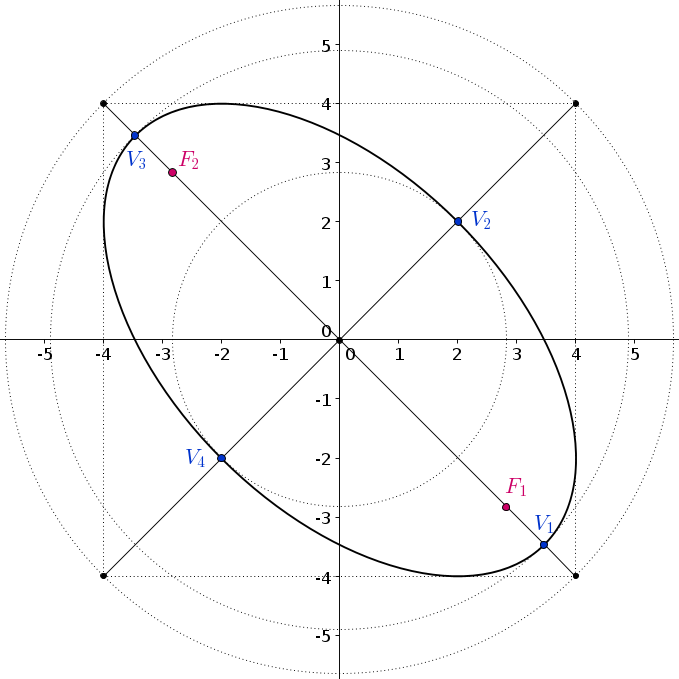
\includegraphics[scale=1.2]{ellisse.png} 
\end{minipage}
\begin{minipage}{0.6\textwidth}
\begin{itemize}
 \item i vertici dell'asse minore si trovano in $\pm(2,2)$
 \item i vertici dell'asse maggiore si trovano in $\pm (2\sqrt{3},-2\sqrt{3})$
 \item i fuochi si trovano in $\pm(2\sqrt{2},-2\sqrt{2})$.
\end{itemize}

Per quanto concerne l'ultima parte abbiamo almeno due approcci possibili. Il primo (puramente geometrico) è ricordare che l'\emph{ortottica} (ossia l'insieme dei punti che ``vedono'' la curva sotto un angolo retto) di una ellisse è una circonferenza di raggio $\sqrt{a^2+b^2}$. Nel nostro caso questo comporta che il quadrato di vertici $(\pm 4,\pm 4)$ sia circoscritto all'ellisse.\\

Alternativamente, per un fissato valore di $y$ si ha che l'equazione $x^2+xy+(y^2-12)=0$ ammette un'unica soluzione se e solo se il discriminante dell'equazione è nullo, ossia se e solo se $y^2=16$.

\end{minipage}


\subsection{Teorema di Taylor e resto integrale}
Sia $I$ un intorno aperto dell'origine e $f$ una funzione di classe $C^d$ su $I$, con $d\geq 1$. Per un qualunque $t\in I$, possiamo considerare che l'applicazione della formula di integrazione produce quanto segue:

\begin{eqnarray*} \int_{0}^{t} (t-x)^{d-1} f^{(d)}(x)\,dx &=&\left[(t-x)^{d-1} f^{(d-1)}(x)\right]_{0}^{t}+(d-1)\int_{0}^{t}(t-x)^{d-2}f^{(d-1)}(x)\,dx\\ &=&-f^{(d-1)}(0)t^{d-1}+(d-1)\int_{0}^{t}(t-x)^{d-2}f^{(d-1)}(x)\,dx. \end{eqnarray*}
Applicando induzione su $d$ ne deduciamo:

$$ \int_{0}^{t} (t-x)^{d-1} f^{(d)}(x)\,dx = -\sum_{k=1}^{d-1}f^{(d-k)}(0) t^{d-k}(d-1)_k + (d-1)!\int_{0}^{t}f'(x)\,dx $$
dove $(d-1)_k$ indica il simbolo di Pochhammer decrescente, ossia $k!\binom{d-1}{k}$.\\ Dividendo ambo i membri per $(d-1)!$ abbiamo quanto segue:

$$ \frac{1}{(d-1)!}\int_{0}^{t}(t-x)^{d-1}f^{(d)}(x)\,dx = -\sum_{j=1}^{d-1}\frac{f^{(j)}(0)}{j!}\,t^j + f(t)-f(0). $$

Una immediata conseguenza è la \textbf{formula di Taylor con resto integrale} per funzioni di classe $C^d$ in un intorno dell'origine:
\begin{theo}[Formula di Taylor con resto integrale]
 $$ f(t) = \sum_{j=0}^{d-1}\frac{f^{(j)}(0)}{j!}\,t^j + \frac{1}{(d-1)!}\int_{0}^{t}(t-x)^{d-1}f^{(d)}(x)\,dx. $$
\end{theo}
Il primo addendo nel membro destro è detto \emph{polinomio di Taylor} di ordine $d-1$, ed è l'unico polinomio di grado $\leq (d-1)$ le cui derivate nell'origine, fino alla $(d-1)$-esima, coincidono con quelle di $f$.\\
Supponendo che $f^{(d)}(x)$ su $[0,t]$ assuma valori compresi tra $m$ ed $M$ abbiamo che il termine di resto è compreso tra $m$ volte ed $M$ volte la seguente quantità:
$$ \frac{1}{(d-1)!}\int_{0}^{t}(t-x)^{d-1}\,dx = \frac{t^d}{d!}. $$
Poiché le funzioni continue hanno la proprietà dei valori intermedi si ha
$$ f(t) = \sum_{j=0}^{d-1}\frac{f^{(j)}(0)}{j!}\,t^j + \frac{t^d}{d!}f^{(d)}(\xi)\quad\text{per qualche }\xi\in(0,t) $$
che è noto anche come \emph{sviluppo di Taylor con resto di Lagrange}. Sottolineiamo che la precedente identità continua a valere sotto ipotesi meno restrittive di quelle qui assunte: è sufficiente che $f^{(d)}$ esista, non è necessario che sia continua. Abbiamo comunque già visto che se $f^{(d)}$ esiste ha automaticamente la proprietà dei valori intermedi (MVP), e sebbene la MVP non comporti automaticamente la Riemann-integrabilità di $(t-x)^{d-1}f^{(d)}(x)$, nei casi concreti è assai raro imbattersi in funzioni che siano derivabili ma non abbiano derivata continua. Inoltre questa impostazione semplicemente basata su integrazione per parti e induzione ha il pregio di produrre una rappresentazione esplicita del resto ed evitare fastidiosi tecnicismi legati alla dimostrazione e all'applicazione del Teorema di De l'H\^opital.\\
Una forma ulteriormente indebolita del resto di Lagrange è data dal resto di Peano, dove la differenza tra $f(t)$ e il suo polinomio di Taylor di ordine $d-1$ è semplicemente espressa come $O(t^d)$. Nei casi in cui si voglia trattare uno sviluppo centrato in un punto $t_0$ diverso dall'origine è sufficiente traslare opportunamente la variabile $t$ e gli argomenti delle derivate di $f$.\\

\emph{Perché gli sviluppi di Taylor sono di fondamentale importanza in Analisi?} Perché permettono di ricondurre l'algebra delle funzioni sufficientemente regolari all'algebra dei polinomi. Nello specifico, perché permettono di
\begin{itemize}
 \item determinare limiti senza dover ricorrere a ripetuti confronti o applicazioni di De l'H\^opital
 \item rappresentare serie come integrali o viceversa (si veda a tal proposito l'esercizio $\textbf{J21}$)
 \item legare il comportamento delle derivate in un punto al comportamento locale o globale della funzione considerata. Il viceversa è ad esempio il problema-cardine in combinatoria analitica, ossia quello di ricostruire il comportamento asintotico di una successione unicamente dalle informazioni algebriche sulla classe combinatoria considerata. All'interno di questo punto rientra anche il problema-cardine della teoria analitica dei numeri, ossia quello di ricostruire la collocazione degli zeri (o dei poli) di certe funzioni a partire dalle equazioni differenziali o funzionali soddisfatte.
\end{itemize}

Prima di avventurarsi in Matematica raffinata è opportuno familiarizzare con i fondamentali, in questo frangente gli sviluppi di Maclaurin (ossia gli sviluppi di Taylor centrati nell'origine) delle funzioni di classe $C^{\infty}$ d'uso comune.

\begin{itemize}
 \item \textbf{Serie geometrica}. Per ogni $x\in(-1,1)$ si ha 
 $$ \frac{1}{1-x}=1+x+x^2+x^3+\ldots = \sum_{n\geq 0}x^n $$
 e in particolare $\left.\frac{d^n}{dx^n}\left(\frac{1}{1-x}\right)\right|_{x=0}=n!$. Rimpiazzando $x$ con $\pm x^d$ si ha che su $(-1,1)$ vale l'identità 
 $$ \frac{1}{1\pm x^d} = \sum_{n\geq 0}(\mp 1)^n x^{nd}. $$
 \item \textbf{Esponenziale, seno e coseno}. Sono funzioni già trattate nell'introduzione, che per ogni $x\in\R$ realizzano 
 $$ e^x = \sum_{n\geq 0}\frac{x^n}{n!},\quad \sin x=\sum_{n\geq 0}\frac{(-1)^n x^{2n+1}}{(2n+1)!}, \quad \cos x=\sum_{n\geq 0}\frac{(-1)^n x^{2n}}{(2n)!}. $$
 Rimuovendo le alternanze di segno nelle ultime due serie si ottengono gli sviluppi di Maclaurin di $\cosh x=\frac{e^x+e^{-x}}{2}$ e $\sinh x=\frac{e^x-e^{-x}}{2}$.
 \item \textbf{Potenze di $1\pm x$}. Dal calcolo esplicito delle derivate nell'origine di $(1+x)^{a}$ si ha che per ogni $x\in(-1,1)$ vale 
 $$ (1+x)^a = \sum_{k\geq 0}\frac{(a)_k}{k!} x^k\qquad\text{dove }(a)_k = a(a-1)\cdot\ldots\cdot (a-k+1) $$
 generalizzando il binomio di Newton a esponenti qualunque. Nel caso di esponenti interi e negativi l'identità 
 $$ \frac{1}{(1-x)^{m+1}} = \sum_{n\geq 0}\binom{n+m}{m} x^n $$
 può anche essere vista come conseguenza dell'espediente combinatorio noto come \emph{Stars\&Bars}.
 \item \textbf{Logaritmo naturale}. Su $(-1,1)$ abbiamo $\frac{d}{dx}\left(-\ln(1-x)\right)=\frac{1}{1-x}$. Per integrazione termine a termine della serie geometrica segue che sul precedente intervallo vale 
 $$ -\ln(1-x) = \sum_{n\geq 1}\frac{x^n}{n}. $$
 Per sommazione per parti (alias \emph{lemma di Abel}) l'identità continua a valere anche nell'estremo sinistro del dominio di convergenza, producendo $\ln 2 = \sum_{n\geq 1}\frac{(-1)^{n+1}}{n}$.
 
\end{itemize}

Alcune considerazioni di simmetria hanno un certo rilievo anche nel contesto delle serie di Fourier: se una funzione di classe $C^\infty$ in un intorno dell'origine è dispari, le sue derivate nell'origine d'ordine pari sono tutte nulle. Analogamente, se una funzione di classe $C^\infty$ in un intorno dell'origine è pari, le sue derivate nell'origine d'ordine dispari sono tutte nulle. La dimostrazione è immediata: è sufficiente considerare l'identità $f(-x)=\pm f(x)$, derivare ambo i membri il corretto numero di volte e infine valutarli in $x=0$.\\

In questo contesto è bene non esagerare con l'ottimismo: per una generica funzione di classe $C^{\infty}$ in un intorno dell'origine, la successione delle derivate nell'origine in generale \textbf{non} fissa la funzione. Consideriamo $\exp(-x^2)$: non è difficile dimostrare che qualunque derivata ha limite zero per $x\to +\infty$ o $x\to -\infty$. Eseguendo la sostituzione $x\to \frac{1}{x}$ ne consegue che 
$$ g(x) = \left\{\begin{array}{rcl}\exp(-1/x^2)&\text{se}&x\neq 0\\ 0 &\text{se}&x=0\end{array}\right. $$
è una funzione di classe $C^\infty$ sull'intera retta reale che ha tutte le derivate nell'origine pari a zero. Tuttavia è palese che $g(x)$ non sia la funzione identicamente nulla, dunque che la successione costantemente nulla non sia associata ad un'unica funzione $C^\infty$ in un intorno dell'origine, ma ad un'intera classe di equivalenza di funzioni $C^\infty$, detta \emph{germe}.\\

Per nostra fortuna \emph{si può} recuperare una corrispondenza biunivoca tra alcune successioni ed alcune funzioni, restringendo opportunamente il grado di regolarità degli oggetti coinvolti. Diciamo che una funzione $f$ è \emph{analitica} (o di classe $C^\omega$) in un intorno $U$ dell'origine se è di classe $C^\infty$ su $U$ e per ogni $x\in U$ esiste una costante $\rho_x > 0$ tale da garantire definitivamente $|f^{(n)}(x)|\leq n! \rho_x^n$. Le quantità $\rho_x$ sono legate a quello che è il \emph{raggio di convergenza} di una serie di potenze, e la limitazione sul modulo delle derivate ci permette di guadagnare uniformità nel termine di resto dell'espansione di Maclaurin. Così facendo ogni successione ``che in modulo non cresce troppo in fretta'' (non più in fretta delle derivate nell'origine di $\frac{1}{1-Rx}$, per qualche $R>0$) risulta essere la successione delle derivate nell'origine di \emph{un'unica} funzione analitica in un intorno dell'origine. Tutto questo sarebbe poco più di una capriola concettuale se le funzioni d'impiego comune non fossero funzioni analitiche (ossia localmente coincidenti con la propria serie di Taylor), ma per fortuna \emph{lo sono}.

\begin{ex} Si determinino la derivata quarta e la derivata quinta nell'origine di $f(x)=\sin(x)\arcsin(x)$. 
\end{ex}
\textbf{Soluzione}. $f(x)$ è una funzione analitica su $(-1,1)$ e pari: in particolare $f^{(V)}(0)={\color{blue}0}$. Il valore di $f^{(IV)}(0)$ è fissato dallo sviluppo di Maclaurin al quart'ordine, ricostruibile a partire da $\sin(x)=x-\frac{x^3}{6}+o(x^4)$ e dallo sviluppo al quart'ordine di $\arcsin x$. Poiché $\frac{d}{dx}\arcsin x = (1-x^2)^{-1/2}$, da 
$$ \frac{1}{\sqrt{1-x}} = \sum_{n\geq 0}\binom{2n}{n}x^n $$
segue 
$$ \frac{1}{\sqrt{1-x^2}}= \sum_{n\geq 0}\binom{2n}{n} x^{2n} $$
e 
$$ \arcsin x = \sum_{n\geq 0}\frac{\binom{2n}{n}}{2n+1}x^{2n+1} = x + \frac{x^3}{6} + o(x^4).$$
Da quanto collezionato segue che al quart'ordine $\sin(x)\arcsin(x)$ è indistinguibile da $\left(x-\frac{x^3}{6}\right)\left(x+\frac{x^3}{6}\right)=x^2+o(x^4)$, dunque anche il valore di $f^{(IV)}(0)$ è $\color{blue}0$.

\newpage

\section{Binomiali \& Friends}
Come spero sia noto il binomiale $\binom{n}{k}$, letto \emph{$n$ su $k$}, rappresenta il numero di sottoinsiemi di cardinalità $k$ in un insieme di $n$ elementi.
Questo è esplicitamente:\\
$$\binom{n}{k} = \frac{n!}{(n-k)!k!}$$    

Proprietà dei binomiali sono: 
\begin{itemize}
    \item \textbf{Binomio di Newton} $(a+b)^n=\sum_{k=0}^{n}\binom{n}{k}a^{n-k}b^k$
    \item $\binom{n}{k}=\binom{n}{n-k}$
    \item $\binom{n+1}{k+1}=\binom{n}{k+1} + \binom{n}{k}$
    \item $2^n= \sum_{k=0}^{n}\binom{n}{k}$
    \item $0 = \sum_{k=0}^{n}\binom{n}{k}(-1)^k$
\end{itemize}

\subsection{Stars \& Bars}
Un importante tecnica di conteggio è appunto \textbf{Stars \& Bars}:
$$\left|\{(x_1,\ldots,x_k)\in(\N^+)^k: x_1+\ldots+x_k = n\}\right|=[x^n]\left(\frac{x}{1-x}\right)^k = \binom{n-1}{k-1},$$
$$ \frac{1}{(1-x)^{k+1}}=\sum_{n\geq 0}\binom{n+k}{k}x^n. $$
L'interpretazione grafica è data dal rispondere alla domanda: in quanti modi possiamo mettere $k-1$ barrette nelle intercapedini tra $n$ oggetti adiacenti? Eccone anche un'applicazione ad un esercizio già visto, ossia la determinazione di $\sum_{n\geq 0}\frac{n^2}{4^n}$. Abbiamo in primo luogo che $n^2$ è certamente una combinazione lineare di $\binom{n+2}{2},\binom{n+1}{1}$ e $\binom{n}{0}=1$.\\ In particolare, per eliminazione gaussiana (o differenze in avanti) vale $n^2=2\binom{n+2}{2}-3\binom{n+1}{1}+\binom{n}{0}$.\\ Da Stars\&Bars segue allora che 

$$ \sum_{n\geq 0} n^2 x^n = \frac{2}{(1-x)^3}-\frac{3}{(1-x)^2}+\frac{1}{1-x} $$

e valutando ambo i membri in corrispondenza di $x=\frac{1}{4}$ si ha immediatamente 

$$ \sum_{n\geq 0}\frac{n^2}{4^n} = 2\left(\frac{4}{3}\right)^3-3\left(\frac{4}{3}\right)^2+\left(\frac{4}{3}\right)=\frac{20}{27}.$$

\subsection{Binomiale centrale}
I coefficienti binomiali centrali sono i binomiali del tipo:
$$\binom{2n}{n}=\frac{(2n)!}{n!^2}=\frac{2^n(2n-1)!!}{n!}$$
così chiamati perché occupano le posizioni centrali del triangolo di Tartaglia.\\ I binomiali centrali figurano nell'\emph{identità di Vandermonde}
$$ \sum_{k=0}^{n}\binom{n}{k}^2 = \sum_{k=0}^{n}\binom{n}{k}\binom{n}{n-k}=[x^n](1+x)^n (1+x)^n = [x^n](1+x)^{2n} = \binom{2n}{n} $$
ed hanno un ruolo chiave nella dimostrazione di Chebyshev della forma debole del Teorema dei numeri primi,\\ $\pi(x)\frac{x}{\ln x}\in [c_1,c_2]$. Seguono disuguaglianze utili per la stima dei binomiali centrali:
    \begin{itemize}
        \item $\frac{4^n}{n+1}\leq\binom{2n}{n}\leq4^n$
        \item $\frac{4^n}{2\sqrt{n}}\leq\binom{2n}{n}\leq\frac{4^n}{\sqrt{3n+1}}$
    \end{itemize}
e ancora più accuratamente $\frac{1}{4^n}\binom{2n}{n}\sim\frac{1}{\sqrt{\pi n}}$ con $\frac{1}{4^n}\binom{2n}{n}\leq \frac{1}{\sqrt{\pi\left(n+\frac{1}{4}\right)}}$.\\ Queste possono essere ricavate dalla rappresentazione integrale 
$$ \frac{1}{4^n}\binom{2n}{n} = \frac{2}{\pi}\int_{0}^{\pi/2}\left(\cos\theta\right)^{2n}\,d\theta. $$
    
\subsection{Hockey Stick Identity}
Vale l'identità:
$$\binom{n+1}{r+1}=\sum_{j=r}^{n}\binom{j}{r}$$
\begin{proof}
 Fissato $r$, è sufficiente procedere per induzione su $n$. In alternativa, è sufficiente catalogare i sottoinsiemi di taglia $r+1$ di $\{1,2,\ldots,n+1\}$ in base al loro elemento massimo.
\end{proof}
Dalla HSI è semplice ricostruire le formule per la somma di potenze consecutive, una cui immediata conseguenza è ad esempio $\int_{0}^{t}x^n\,dx = \frac{t^{n+1}}{n+1}$ per ogni $t\in\R$ ed ogni $n\in\N$. Vediamo il caso $n=3$:
\begin{ex}[Identità di Nicomaco] Si determini esplicitamente, in funzione di $N$, il valore della somma 
$$ \sum_{n=1}^{N} n^3. $$
 
\end{ex}
\textbf{Soluzione}. Osserviamo che $n^3$ è un polinomio di grado $\leq 3$ della variabile $n$, così come $\binom{n}{k}$ per $k\in[0,3]$.\\ In particolare $n^3$ è una combinazione lineare a coefficienti costanti dei precedenti binomiali, $n^3=\sum_{k=0}^{3}\binom{n}{k}c_k$.\\
I valori dei coefficienti $c_k$ possono essere ricostruiti per eliminazione, o più efficientemente per differenze in avanti:
$$\begin{array}{ccccccc} 0 && 1 && 8 && 27 \\ 
& 1 && 7 && 19 & \\
&& 6 && 12 && \\
&&& 6 &&&
\end{array} $$
fornisce $n^3=6\binom{n}{3}+6\binom{n}{2}+1\binom{n}{1}$ (i coefficienti così trovati sono legati ai \emph{numeri di Stirling del secondo tipo}).\\ Dalla HSI abbiamo pertanto
$$ \sum_{n=1}^{N}n^3 = 6\sum_{n=1}^{N}\binom{n}{3}+6\sum_{n=1}^{N}\binom{n}{2}+\sum_{n=1}^{N}\binom{n}{1}=6\binom{N+1}{4}+6\binom{N+1}{3}+\binom{N+1}{2}={\color{blue}\left(\frac{N(N+1)}{2}\right)^2}=\left(\sum_{n=1}^{N}n\right)^2.$$

\newpage

    \section{Criteri e metodi per serie numeriche}
    \subsection{Serie importanti}
Seguono le più importanti serie numeriche convergenti, utili nella stima di altre serie e nella verifica della loro convergenza.\\
\textbf{Serie armonica generalizzata}
$$\sum_{n=0}^{\infty}\frac{1}{n^\alpha}$$
è una serie convergente se e solo se
$\alpha\in\R>1$. La dimostrazione è lasciata come \textbf{importante} esercizio.
\\
\textbf{Serie geometrica}
$$S=\sum_{n=0}^{\infty}x^n$$
Ha il seguente comportamento:
\begin{equation*}
\begin{cases}
    |x|\in(0,1) \rightarrow S=\frac{1}{1-x}
    \\x \geq 1 \rightarrow S=\infty
    \\x\leq -1 \rightarrow \not\exists S
    
\end{cases}
\end{equation*}
\textbf{Serie telescopica}
Ogni somma/serie in cui il termine generale si può esprimere come differenza di termini consecutivi (o quasi) si calcola, infatti vale
$$\sum_{n=0}^{N}\left(a_n - a_{n+1}\right) = a_0 - a_{N+1}$$
per massiccia cancellazione: il membro sinistro corrisponde alla differenza tra la prima quantità sommata e l'ultima quantità sottratta.

\subsection{Criteri}
Seguiranno i principali criteri di convergenza per le Serie.
\subsubsection{Serie a termini definitivamente non negativi}
\textbf{Criterio del confronto} \\
Sia
$$\sum_{n=0}^{\infty}a_n<\infty$$
Se vale che definitamente $0\leq b_n\leq a_n$, allora
$$\sum_{n=0}^{\infty}b_n<\infty.$$
Eventualmente in combinazione con somme telescopiche, questo criterio prova la convergenza o divergenza di molte serie. Ad esempio da $\frac{1}{n^2}<\frac{1}{n(n-1)}$ segue 
$$ \sum_{n\geq 1}\frac{1}{n^2} = 1+\sum_{n\geq 2}\frac{1}{n^2} \leq 1+\sum_{n\geq 2}\left(\frac{1}{n-1}-\frac{1}{n}\right) = 2 $$
e un discorso analogo può essere applicato anche alla serie armonica generalizzata.\\

\textbf{Criterio del confronto asintotico} \\
È una forma più generale del precedente criterio. Se due successioni a termini non negativi $\{a_n\}_{n\geq 1}$ e $\{b_n\}_{n\geq 1}$ \\sono tali per cui $\lim_{n\to+\infty}\frac{a_n}{b_n}$ esiste finito, le serie 
$$ \sum_{n\geq 1} a_n,\qquad \sum_{n\geq 1} b_n $$
sono entrambe convergenti o entrambe positivamente divergenti.\\

\textbf{Criterio del rapporto} \\
Sia
$$\sum_{n=0}^{\infty}a_n$$
una serie a termini mai nulli. Se si ha che:
$$\lim_{n\to\infty} \left|\frac{a_{n+1}}{a_n}\right|=c<1$$
allora la serie degli $a_n$ converge assolutamente.\\
È una conseguenza abbastanza immediata della definizione di limite e del criterio del confronto.\\ O, volendo, del criterio successivo, in quanto per il Lemma di Hadamard $\frac{|a_{n+1}|}{|a_n|}\to c$ comporta $\sqrt[n]{|a_n|}\to c$.\\

\textbf{Criterio della radice} \\
Se $\{a_n\}_{n\geq 1}$ è una successione a valori non negativi tale per cui
$$ \lim_{n\to +\infty}\sqrt[n]{a_n} = c \in [0,1), $$
allora la serie $\sum_{n\geq 1}a_n$ converge.\\
È una conseguenza immediata del confronto con una serie geometrica convergente.\\

\textbf{Criterio serie-integrale} \\
Se $f:[1,+\infty)\to\mathbb{R}$ è una funzione non negativa e debolmente decrescente, la serie $\sum_{n\geq 1}f(n)$ converge se e solo se $f$ è impropriamente Riemann-integrabile su $[1,+\infty)$. Per additività dell'integrale e monotonia dell'integranda si ha infatti, per ogni $N\in\N^+$: 
$$ \sum_{n=1}^{N}f(n) \geq \int_{1}^{N+1}f(x)\,dx $$
come anche 
$$ \sum_{n=1}^{N}f(n) \leq f(1)+\int_{1}^{N}f(x)\,dx.$$
Nel caso in cui $f$ sia convessa la disuguaglianza di Hermite-Hadamard \ref{HermiteHadamard} fornisce stime anche più precise.

\subsubsection{Serie a termini di segno variabile}

\textbf{Criterio di Leibniz}\\
Se $\{a_n\}_{n\geq 0}$ è una successione decrescente a zero, la serie
$$ \sum_{n\geq 0} (-1)^n a_n $$
è convergente.\\
\begin{proof} Posto come di consueto $A_N=\sum_{n=0}^{N}a_n$, dalle ipotesi segue che $\{A_{2N}\}_{N\geq 0}$ è una successione decrescente mentre $\{A_{2N+1}\}_{N\geq 0}$ è una successione crescente. Poiché $A_{2N} > A_{2N+1}$ le due successioni sono entrambe convergenti, in quanto quella crescente è limitata dall'alto mentre quella decrescente è limitata dal basso. Inoltre i limiti di queste due successioni debbono coincidere, in quanto $A_{2N+1}-A_{2N}=a_{2n+1}$ converge a zero per ipotesi. Segue che l'intera successione delle somme parziali è convergente, ossia che la serie è convergente. 
\end{proof}


Una importante generalizzazione è data dal \textbf{Criterio di (Abel-)Dirichlet}.\\
Se $\{a_n\}_{n\geq 0}$ è una successione con somme parziali limitate e $\{b_n\}_{n\geq 0}$ è una successione decrescente a zero,\\ la serie $\sum_{n\geq 0}a_n b_n$ è convergente.

\emph{Sketch della dimostrazione}. Segue dall'identità
$$ \sum_{n=0}^{N}a_n b_n = A_N b_N - \sum_{n=0}^{N-1} A_n (b_{n+1}-b_n) $$
che è un analogo discreto della formula di integrazione per parti, nota come \textbf{formula di sommazione per parti}.\\ La sua dimostrazione è banale per induzione su $N$.\qed

Dalla formula di integrazione per parti segue l'omonimo criterio per gli integrali: se su $[0,+\infty)$ si ha che $f(x)$ ha primitiva limitata e $g(x)$ è decrescente a zero, $f(x)g(x)$ è impropriamente Riemann-integrabile su $\R^+$.

\subsection{Serie di potenze}
Una serie di potenze (centrata nell'origine) è definita come:
$$\sum_{n=0}^{\infty}a_n x^n$$
con $x\in\C$, e sia il \textbf{raggio di convergenza} \\
$$\rho=\frac{1}{\limsup\sqrt[n]{|a_n|}}.$$
La serie di potenze converge puntualmente nella palla $B_0=\left\{z\in\C : |z|< \rho \right\}$ e uniformemente su ogni compatto contenuto in $B_0$.

\subsection{Metodi creativi per il calcolo esplicito}
Vediamo adesso come abusare della linearità delle serie per calcolare esplicitamente una classe di queste. \\
Sia
$$S=\sum_{n\geq 0}^{}\frac{f(n)}{k^n}$$
con $k\in\N \wedge k\geq 2$.
Sarebbe molto comodo in questo caso ricondursi ad una serie geometrica.
Ipotizzando che esista una applicazione lineare e continua $T$ tale da mandare $x^n$ in $f(n)$ otteniamo:
$$S=\sum_{n\geq 0}\frac{f(n)}{k^n}=\sum_{n\geq 0}\frac{T(x^n)}{k^n}= T\left(  \sum_{n\geq 0}\left(\frac{x}{k}\right)^n \right)= T \left(\frac{1}{1-\frac{x}{k}}\right)$$ \\
in base alla scelta/costruzione di $T$ possiamo calcolare esplicitamente tutte le serie di questo tipo.
(Possibili applicazioni lineari che farebbero al caso nostro sono: derivazione, integrazione, somma, prodotto, valutazione e tutte le loro composizioni)\\
Un esempio di utilizzo di questo metodo è calcolare esplicitamente la serie:
$$\sum_{n\geq 0}^{}\frac{n^2}{4^n}$$
utilizzando come operatore $T$ la somma delle prime due derivate valutata in $1$ (esercizio per il lettore).\\
In generale questo metodo è utile ogni qual volta si sta trattando una serie i cui termini, a meno di un fattore, coincidono con quelli di una serie che già sappiamo calcolare.\\
A onor del vero, per quanto potente è raro che tale metodo sia \emph{l'unico} in grado di esplicitare un'assegnata serie. 
Tornando all'esempio precedente, è ovvio che la serie presentata sia convergente, in quanto definitivamente $\frac{n^2}{4^n}\in\left(0,\frac{1}{3^n}\right]$. 
Sono allora lecite tutte le seguenti manipolazioni (basate unicamente su moltiplicazioni per $4$ e \emph{reindexing}):
$$ S=\sum_{n\geq 0}\frac{n^2}{4^n}=\sum_{n\geq 1}\frac{n^2}{4^n},\qquad 4S=\sum_{n\geq 1}\frac{n^2}{4^{n-1}}=\sum_{m\geq 0}\frac{(m+1)^2}{4^m}, $$

$$ 3S=4S-S = \sum_{n\geq 0}\frac{(n+1)^2-n^2}{4^n}=\sum_{n\geq 0}\frac{2n+1}{4^n}=1+\sum_{n\geq 1}\frac{2n+1}{4^n},$$

$$ 12S=4(3S) = 4+\sum_{n\geq 1}\frac{2n+1}{4^{n-1}} = 4+\sum_{m\geq 0}\frac{2m+3}{4^m}, $$

$$ 9S = 12S-3S = 4+\sum_{n\geq 0}\frac{(2n+3)-(2n+1)}{4^n} = 4+2\sum_{n\geq 0}\frac{1}{4^n} = 4+\frac{2}{1-\frac{1}{4}} = 4+\frac{8}{3} = \frac{20}{3} $$
dalle quali segue $S=\frac{20}{27}$.


\subsubsection{Criterio di convergenza dominata}

Per il \textbf{Teorema di convergenza dominata} tutte le serie che convergono \emph{abbastanza} velocemente commutano con l'integrale. All'atto pratico ciò comporta che, nelle ipotesi corrette, è lecito scrivere:
$$\sum_{n\geq 0}^{}\int_{a}^{b}f_n(x)\,dx =\int_{a}^{b}\sum_{n\geq 0} f_n(x)\, dx.$$ 
Questo torna utile in quanto è moderatamente comune sostituire ad una funzione una sua \textbf{rappresentazione integrale}, come ad esempio nella soluzione dell'esercizio \textbf{J17}, o del seguente.

\begin{ex} Si determini esplicitamente il valore della serie 
$$ \sum_{n\geq 1}\frac{1}{n^2+1}. $$
 
\end{ex}
\textbf{Soluzione}. È pratico osservare preliminarmente che, per integrazione per parti,
$$ \frac{1}{n^2+1} = \int_{0}^{+\infty}\frac{\sin(nx)}{n}\,e^{-x}\,dx.$$
Poiché $\sum_{n\geq 1}\frac{z^n}{n}=-\log(1-z)$ vale per ogni $z\in\C$ di modulo $<1$, dal Lemma di Abel segue che $\operatorname{Im}\sum_{n\geq 1}\frac{e^{inx}}{n}=\sum_{n\geq 1}\frac{\sin(nx)}{n}$ è il prolungamento $2\pi$-periodico della funzione che su $(0,2\pi)$ vale $\frac{\pi-x}{2}$ (\emph{onda a dente di sega} o \emph{sawtooth wave}). Invocando il Teorema di convergenza dominata abbiamo la seguente catena di uguaglianze:
\begin{eqnarray*}
 \sum_{n\geq 1}\frac{1}{n^2+1}&=&\int_{0}^{+\infty}e^{-x}\sum_{n\geq 1}\frac{\sin(nx)}{n}\,dx = \int_{0}^{+\infty}e^{-x}\left(\frac{\pi-x}{2}\right)_{\text{per}}\,dx = \frac{1}{1-e^{-2\pi}}\int_{0}^{2\pi}\left(\frac{\pi-x}{2}\right)e^{-x}\,dx \\
 &=& \frac{e^{\pi}}{e^{2\pi}-1}\int_{-\pi}^{\pi}\frac{x}{2}e^{-x}\,dx = \frac{e^{\pi}}{e^{2\pi}-1}\int_{0}^{\pi}x\sinh(x)\,dx = \frac{e^\pi}{e^{2\pi}-1}\left(\left[x\cosh x\right]_{0}^{\pi}-\left[\sinh x\right]_{0}^{\pi}\right)\\
 &=& \frac{e^\pi}{e^{2\pi}-1}\left(\pi\frac{e^\pi+e^{-\pi}}{2}-\frac{e^\pi-e^{-\pi}}{2}\right) = \frac{\pi}{2}\cdot \frac{e^{2\pi}+1}{e^{2\pi}-1}-\frac{1}{2}={\color{blue}\frac{\pi\coth\pi-1}{2}}.\qed
\end{eqnarray*}

L'espediente appena utilizzato può essere generalizzato, dando luogo a quanto noto come \emph{formula di sommazione di Poisson}.
\subsubsection{Creative telescoping}
Un metodo importante è quello di trasformare serie apparentemente complesse in serie telescopiche o combinazioni lineari di serie telescopiche.
Tipicamente per questo tipo di lavoro bisogna farci l'occhio e sapere un po' dove mettere le mani, ma diventa abbastanza intuitivo velocemente (serve appunto un po' di creatività). Un esempio classico riguarda il problema di Basilea, ossia la determinazione di $\zeta(2)=\sum_{n\geq 1}\frac{1}{n^2}$. Il termine generale della serie non è evidentemente telescopico, ma è prossimo a quello della serie di Mengoli, da cui:
$$ \sum_{n\geq 1}\frac{1}{n^2} = \sum_{n\geq 1}\frac{1}{n(n+1)}+\sum_{n\geq 1}\frac{1}{n^2(n+1)} = 1+\sum_{n\geq 1}\frac{1}{n^2(n+1)}. $$
Alla ``serie residua'' che costituisce l'ultimo termine possiamo applicare una manipolazione analoga, eventualmente scorporando il primo addendo. Ciò conduce a 
$$ \zeta(2) = 1+\sum_{n\geq 1}\frac{1}{n(n+1)(n+2)}+2\sum_{n\geq 1}\frac{1}{n^2(n+1)(n+2)} = 1+\frac{1}{4}+2\sum_{n\geq 1}\frac{1}{n^2(n+1)(n+2)}. $$
Iterando il processo si ottiene l'identità 
$$ \zeta(2)=\sum_{n\geq 1}\frac{1}{n^2} = 3\sum_{n\geq 1}\frac{1}{n^2\binom{2n}{n}}$$
in cui le somme parziali dell'ultima serie convergono sensibilmente più in fretta delle somme parziali della serie originaria, poiché $\binom{2n}{n}\sim \frac{4^n}{\sqrt{\pi n}}$. Parliamo in questi casi di \emph{accelerazione} di serie convergenti. Dalle rappresentazioni integrali dei binomiali centrali abbiamo inoltre che l'ultima identità comporta
$$ \zeta(2) = \frac{3}{2}\int_{0}^{1}\sum_{m\geq 0}\frac{(x(1-x))^{m}}{m+1}\,dx = \frac{3}{2}\int_{0}^{1}-\log(1-x+x^2)\left(\frac{1}{x}+\frac{1}{1-x}\right)\,dx \stackrel{\text{sym}}{=}3\int_{0}^{1}\frac{-\log\Phi_6(x)}{x}\,dx $$
o, via integrazione per parti, $\zeta(2)=3\int_{0}^{1}\frac{2x-1}{1-x+x^2}\log(x)\,dx$. Sebbene Eulero non abbia seguito questa strada, e sebbene sia tecnicamente più semplice applicare l'identità di Parseval a serie di Fourier elementari, da qui si può giungere senza atroci intoppi a provare che $\zeta(2)=\frac{\pi^2}{6}$. La fabbricazione di serie accelerate, in cui il termine generale abbia decorose proprietà aritmetiche, riveste una certa importanza anche in \emph{approssimazione diofantea}, in quanto permette in alcune circostanze di dimostrare l'irrazionalità di fissate costanti. Apery si è ad esempio servito di 
$$ \zeta(3) = \frac{5}{2}\sum_{n\geq 1}\frac{(-1)^{n+1}}{n^3\binom{2n}{n}} $$
per dimostrare nel 1977 che $\zeta(3)\not\in\Q$.\\ La presunta irrazionalità di $\zeta(5),\gamma,\Gamma\left(\frac{1}{5}\right)$ (e molte altre costanti) è tuttora una questione aperta.

\section{Integrazione secondo Riemann}
Questo paragrafo, dopo un breve recap, si concentrerà nell'illustrare degli integrali più complessi e meritevoli di particolare attenzione, oltre che a tecniche di integrazione un po' più oscure. Ad avviso mio e di Jack, i metodi che mostreremo sono abbastanza importanti da avere a portata di mano in caso di necessità. Alcuni argomenti che saranno trattati sono l'utilizzo della convergenza dominata (vedere paragrafo sui criteri delle serie), Integrali complessi, \emph{abuso} di rappresentazioni integrali etc.
\begin{definizione}[Partizione] Dato un intervallo chiuso e limitato della retta reale $[a,b]$, una qualunque sequenza 
$$ a=a_0 < a_1 < \ldots < a_n = b $$
definisce una \textbf{partizione} di $[a,b]$:
$$ [a,b]=\bigcup_{k=1}^{n} I_k,\qquad I_k=[a_{k-1},a_{k}]. $$ 
\end{definizione}
\begin{definizione}[Calibro o finezza] Il \emph{calibro} o \emph{finezza} di una partizione è la massima lunghezza degli intervalli che costituiscono la partizione. 
\end{definizione}
\begin{definizione}[Ordinamento parziale delle partizioni] Date due partizioni $\mathcal{P}_1$ e $\mathcal{P}_2$ dello stesso intervallo, diciamo che $\mathcal{P}_1$ \emph{è più fine} di $\mathcal{P}_2$, in simboli $\mathcal{P}_1 \geq \mathcal{P}_2$, se gli estremi degli intervalli di $\mathcal{P}_1$ costituiscono una sottosequenza degli estremi degli intervalli di $\mathcal{P}_2$. Questo definisce una relazione d'ordine parziale sull'insieme delle partizioni: date due distinte partizioni $\mathcal{P}_1,\mathcal{P}_2$, non è detto che $\mathcal{P}_1$ sia più fine di $\mathcal{P}_2$ o viceversa. Tuttavia, date due distinte partizioni $\mathcal{P}_1,\mathcal{P}_2$, esiste sempre una partizione $\mathcal{P}_3$ più fine di entrambe: è sufficiente prendere gli estremi degli intervalli di $\mathcal{P}_3$ come quelle quantità che sono un estremo di un intervallo di $\mathcal{P}_1$ o (inclusivo) di $\mathcal{P}_2$.
\end{definizione}
L'\textbf{integrale di Riemann} in senso proprio si definisce a partire da $f:[a,b]\to\R$ limitate.

\begin{definizione}[Somme di Riemann superiori e inferiori]
Data una $f$ siffatta e una partizione $\mathcal{P}=\bigcup_{k=1}^{n}I_k$ di $[a,b]$, definiamo la \textbf{somma di Riemann superiore} $S^+_{\mathcal{P}}(f)$ e la  \textbf{somma di Riemann inferiore} $S^-_{\mathcal{P}}(f)$ nel seguente modo:

$$ S^+_{\mathcal{P}}(f) = \sum_{k=1}^{n} \mu(I_k) \sup_{x\in I_k} f(x), \qquad S^-_{\mathcal{P}}(f) = \sum_{k=1}^{n} \mu(I_k) \inf_{x\in I_k} f(x)$$
dove $\mu(I_k)$ denota la lunghezza di $I_k$, ossia $a_{k}-a_{k-1}$.
\end{definizione}

Seguono alcuni lemmi di immediata dimostrazione ma di cruciale importanza:
\begin{itemize}
 \item Per qualunque partizione $\mathcal{P}$ si ha $S^+_{\mathcal{P}}\geq S^-_{\mathcal{P}}$
 \item Se $\mathcal{P}_2$ è più fine di $\mathcal{P}_1$, $S^+_{\mathcal{P}_2} \leq S^+_{\mathcal{P}_1}$
 \item  Se $\mathcal{P}_2$ è più fine di $\mathcal{P}_1$, $S^-_{\mathcal{P}_2} \geq S^+_{\mathcal{P}_1}$
\end{itemize}

\begin{definizione}[Integrale di Riemann]
I precedenti lemmi comportano l'esistenza e la finitezza sia di $\sup_{\mathcal{P}}S^-_{\mathcal{P}}$, detto \emph{integrale di Riemann inferiore}, che di $\inf_{\mathcal{P}}S^+_{\mathcal{P}}$, detto \emph{integrale di Riemann superiore}. È automatico che l'integrale di Riemann inferiore sia $\leq$ dell'integrale di Riemann superiore, ma non è affatto automatico che tali quantità coincidano. Se coincidono, $f$ è detta \emph{Riemann-integrabile} su $[a,b]$ e il valore di $\sup_{\mathcal{P}}S^-_{\mathcal{P}}=\inf_{\mathcal{P}}S^+_{\mathcal{P}}$ è denotato come 
$$ \int_{a}^{b} f(x)\,dx. $$
\end{definizione}

\begin{theorem} Ogni $f\in C^0([a,b])$ è Riemann-integrabile su $[a,b]$ e realizza 
$$ \int_{a}^{b} f(x)\,dx = \lim_{N\to +\infty}\frac{b-a}{N}\sum_{k=1}^{N}f\left(a+\frac{k}{N}(b-a)\right) = \lim_{N\to +\infty}\frac{b-a}{N}\sum_{k=0}^{N-1}f\left(a+\frac{k}{N}(b-a)\right).$$
\end{theorem}
\begin{proof} Per Heine-Cantor $f$ è uniformemente continua su $[a,b]$, ossia per ogni $\epsilon > 0$ esiste un $\delta > 0$ che assicura 
$$ |x_1-x_2|\leq \delta\quad\Longrightarrow\quad |f(x_1)-f(x_2)|\leq \varepsilon.$$
Per qualunque partizione $\mathcal{P}$ di calibro $\leq \delta$ si ha pertanto che 
$$ S^+_{\mathcal{P}}- S^-_{\mathcal{P}} = \sum_{k=1}^{n}\mu(I_k)\left(\sup_{x\in I_k}f(x)-\inf_{x\in I_k}f(x)\right)= \sum_{k=1}^{n}\mu(I_k)\left(\max_{x\in I_k}f(x)-\min_{x\in I_k}f(x)\right)\leq \sum_{k=1}^{n}\mu(I_k)\epsilon = \epsilon (b-a). $$
Data l'arbitrarietà di $\epsilon$ si ha che l'integrale di Riemann inferiore e l'integrale di Riemann superiore hanno distanza arbitrariamente piccola, cioè nulla, visto che $\R$ è un campo archimedeo, dunque privo di infinitesimi. Ciò comporta la Riemann-integrabilità di $f$. L'uniforme continuità di $f$ comporta anche che l'integrale $\int_{a}^{b} f(x)\,dx$ coincida con il $\sup_{\mathcal{P}\in U} S^-_{\mathcal{P}}$ e con l'$\inf_{\mathcal{P}\in U} S^+_{\mathcal{P}}$ sull'insieme $U$ delle \emph{partizioni uniformi}, ossia quelle in cui tutti gli intervalli hanno lunghezza pari al calibro. All'interno dell'insieme di queste partizioni, nuovamente per uniforme continuità di $f$, sia 

$$ S^+_{\mathcal{P}}-\sum_{k=1}^{n}\mu(I_k) f(\max I_k)\quad\text{che}\quad S^-_{\mathcal{P}}-\sum_{k=1}^{n}\mu(I_k) f(\min I_k) $$
possono essere resi arbitrariamente vicini a zero in modulo. Questo prova le ultime due uguaglianze. 
\end{proof}
\begin{definizione}
    Sia $I$ un intervallo di $\R$, e sia $f:I\to\R$ una funzione. Si dice che $F:I\to\R$ è una \emph{primitiva}\\ (o \emph{antiderivata}) di $f$ su $X$ se per ogni $x\in X$ $F$ è derivabile e $F'(x)=f(x)$. $F(x)$ si denota inoltre come $\int f(x)\,dx. $
\end{definizione}

\textbf{Nota}: una primitiva è fissata a meno dell'addizione di una costante arbitraria.\\ Per intenderci, sia $-\cos(x)$ che $2\sin^2\left(\frac{x}{2}\right)=1-\cos(x)$ sono primitive di $\sin(x)$.

\begin{theorem} 
Per funzioni $f,g$ Riemann-integrabili sull'intervallo $I$ valgono le seguenti proprietà:
:
\begin{itemize}
    \item $$\int_{I} (f+g)(x)\,dx = \int_{I} f(x) + \int_{I} g(x)$$
    \item $$\forall\alpha\in\R\qquad \int_{I} \alpha f(x)\,dx =\alpha\int_{I} f(x)\,dx$$
    \item $$\text{se } f\leq g \Rightarrow \int_{I}f(x)\,dx \leq \int_{I}g(x)\,dx$$
\end{itemize}
Questo si traduce nel fatto che l'operatore $\int$ è \emph{lineare} e \emph{monotono}.
\end{theorem}
\begin{theorem}
    Sia $[a,b]\in\R$ un intervallo e sia $f:[a,b]\to\R$ Riemann-integrabile in $[a,b]$ e sia $c\in[a,b]$ fissato.\\ Vale che:\\
    1) La funzione integrale di $f$ di punto iniziale $c$, $\int_c^x f(t)\,dt$ è localmente lipschitziana e quindi continua in $[a,b]$ \\
    2) (Torricelli) Se $f$ è continua in $x\in[a,b]$ allora $\int_c^x f(t)\,dt$ è derivabile in $x$ e si ha: $$\left(\int_c^x f(t)\,dt\right)' =f(x).$$
\end{theorem}
\begin{proof}
    Iniziamo a dimostrare la continuità. Sia $[a,b]$ un intervallo fissato, sia $\lambda=\sup_{x\in[a,b]}|f(x)|$.\\ Mostriamo che $\lambda$ è la costante di Lipschitz cercata su $[a,b]$:
    $$\left|\int_c^xf(x_2)\,dx-\int_c^xf(x_1)\,dx\right|=\left|\int_{x_1}^{x_2}f(t)\,dt\right|\leq\left|\int_{x_1}^{x_2}|f(t)|\,dt\right|\leq\left|\int_{x_1}^{x_2}\lambda dt\,\right|=\lambda|x_2-x_1|$$
    Introduciamo per semplicità la notazione: $\int_c^xf(t)\,dt= I_c f(x).$ \\
    Per quanto riguarda la parte dovuta a Torricelli bisogna provare che: 
    $$\lim_{h\to x}\left|\frac{I_cf(h)-I_cf(x)}{h-x}-f(x)\right|=0.$$
    Bisogna quindi dimostrare che fissato $\epsilon>0$ esiste $\delta>0$ tale che:
    $$\left|\frac{I_cf(h)-I_cf(x)}{h-x}-f(x)\right|\leq\epsilon\quad \text{ se }  0<|h-x|\leq\delta, h\in[a,b]$$
    $I_cf(h)-I_cf(x)$ si può scrivere come $\int_x^hf(t)dt$, inoltre 
    $$f(x)=f(x)\cdot 1 = f(x)\left(\frac{1}{h-x}\int_x^h dt\right)=\frac{1}{h-x}\int_x^h f(x)\,dt.$$
    Essendo $f(x)$ costante rispetto alla variabile di integrazione $t$ si ha che:
    $$\left|\frac{I_cf(h)-I_cf(x)}{h-x}-f(x)\right|=\left|\frac{1}{h-x}\int_x^h f(t)\,dt -\frac{1}{h-x}\int_x^h f(x)\,dt\right|$$
    $$=\frac{1}{|h-x|}\left|\int_x^h(f(t)-f(x))\,dt\right|\leq\frac{1}{|h-x|}\left|\int_x^h|f(t)-f(x)|\,dt\right|.$$
    Essendo $f$ per ipotesi continua in $x$ vale che $|f(h)-f(x)|\leq\epsilon$ se $h\in[a,b]$ tale che $0<h-x\leq\delta$. Si ha quindi:
    $$\frac{1}{|h-x|}\left|\int_x^h|f(t)-f(x)|\,dt\right|\leq\frac{1}{|h-x|}\left|\int_x^h\epsilon\, dt\right|=\frac{1}{|h-x|}\epsilon|h-x|=\epsilon.$$
\end{proof}
Dopo tutta questa fatica, almeno, il teorema seguente è gratuito.
\begin{theorem}[Teorema Fondamentale del Calcolo Integrale]
Sia $f:[a,b]\to\R$ una funzione integrabile secondo Riemann. Allora l'insieme degli integrali indefiniti di $f$ coincide con l'insieme delle primitive di $f$, ovvero: $$F(x)=c+\int_c^x f(t)\,dt.$$    
\end{theorem}
\begin{proof}
    Assumendo $c\in [a,b]$ si ha che $\int_{a}^{b}f = F + c$, che differisce da tutte le altre primitive per una costante. Per la continuità di $f$ e per il punto $2$ del teorema precedente si conclude.
\end{proof}

Nella determinazione esplicita della primitiva di una funzione è spesso opportuno o necessario utilizzare sostituzioni. Il seguente risultato ne regola la meccanica.

\begin{theo}[Cambio di variabile]
Supponiamo che $f:[a,b]\to\R$ sia continua e\\ $\varphi:[c,d]\to[a,b]$ sia un'applicazione di classe $C^1$ con inversa di classe $C^1$. In queste ipotesi si ha
$$ \int_{a}^{b} f(x)\,dx \stackrel{x\mapsto\varphi(t)}{=}\int_{c}^{d}\varphi'(t) f(\varphi(t))\,dt = \int_{\varphi^{-1}(a)}^{\varphi^{-1}(b)}\varphi'(t) f(\varphi(t))\,dt.$$
\end{theo}
\begin{proof}
Cominciamo con l'osservare che la tesi è ovvia nel caso in cui $\varphi$ sia una mappa affine e invertibile, $\varphi(t)=mt+q$ con $m\neq 0$:

$$ \int_{a}^{b}f(x)\,dx = \int_{a-q}^{b-q}f(y+q)\,dy = m \int_{\frac{a-q}{m}}^{\frac{b-q}{m}}f(mt+q)\,dt = \int_{\varphi^{-1}(a)}^{\varphi^{-1}(b)}\varphi'(t) f(\varphi(t))\,dt.$$
Per le proprietà algebriche dell'integrale la tesi resta vera nel caso in cui $\varphi:[c,d]\to[a,b]$ sia una funzione continua, lineare a tratti e strettamente monotona: in tal caso il grafico di $\varphi$ è una spezzata e $\varphi^{-1}$ è a sua volta una funzione continua, lineare a tratti e strettamente monotona. In questo caso $\varphi'(t)$ può non essere definita negli estremi dei lati della spezzata, ma poiché l'insieme dei punti di non derivabilità di $\varphi$ è un insieme discreto, il valore dell'integrale non ne risente. In virtù di quanto osservato, non è restrittivo assumere che nelle ipotesi del teorema che si abbia $[c,d]=[0,1]$. Dato $\varphi:[0,1]\to[a,b]$ diffeomorfismo di classe $C^1$, definiamo una sua approssimazione 

$$\varphi_n(t) = (1-\lambda)\varphi\left(\frac{\lfloor nt\rfloor}{n}\right)+\lambda \varphi\left(\frac{\lceil nt\rceil }{n}\right),\qquad \lambda= t-\frac{\lfloor nt\rfloor}{n} $$
che ha per grafico una spezzata ed è una funzione continua, lineare a tratti e strettamente monotona. Laddove è definita (ossia su tutto l'intervallo $[0,1]$, a meno dell'insieme discreto dato dai multipli interi di $\frac{1}{n}$) $\varphi_n'(t)$ dista da $\varphi'(t)$ al più il modulo di continuità di $\varphi'$ su intervalli di lunghezza $\frac{1}{n}$. Segue che $\varphi_n(t)$ converge uniformemente a $\varphi(t)$ su $[0,1]$ e si ha 

$$ \int_{a}^{b} f(x)\,dx = \int_{0}^{1}\varphi_n'(t)f(\varphi_n(t))\,dt = \lim_{n\to +\infty}\int_{0}^{1}\varphi_n'(t)f(\varphi_n(t))\,dt = \int_{0}^{1}\lim_{n\to +\infty}\varphi_n'(t)f(\varphi_n(t))\,dt = \int_{0}^{1}\varphi'(t)f(\varphi(t))\,dt.$$

\end{proof}

\textbf{Nota}: la dimostrazione appena esposta si estende abbastanza agilmente al caso di funzioni di più variabili. Inoltre l'idea di approssimare funzioni sufficientemente regolari con funzioni lineari a tratti può essere utilizzata (come fatto da Lebesgue) anche per dimostrare quanto segue:

\begin{theorem}[Di approssimazione di Weierstrass]. Rispetto alla norma del $\sup$ i polinomi sono densi in $C([a,b])$. In termini equivalenti, per qualunque funzione continua $f:[a,b]\to\R$ e per qualunque $\epsilon > 0$ esiste un polinomio $p(x)$ che realizza $|f(x)-p(x)|\leq\epsilon$ per ogni $x\in[a,b]$. 
\end{theorem}

Alla luce di questo risultato di \emph{densità}, in molti esercizi teorici sull'integrabilità secondo Riemann non è restrittivo supporre che la funzione integranda sia polinomiale.


\subsection{Sostituzioni da ricordare}
Nella pratica è piuttosto frequente imbattersi in integrali dove la funzione integranda coinvolge la radice quadrata di un polinomio di secondo grado. A seconda che tale polinomio abbia discriminante positivo o negativo è opportuno ricordare alcune sostituzioni notevoli.
\begin{itemize}
 \item (Discriminante negativo) La gestione del termine $\sqrt{x^2+1}$ è semplificata dalla sostituzione $x=\tan\theta$ o dalla sostituzione $x=\sinh t$. In un intorno dell'origine abbiamo infatti $\sqrt{\tan^2\theta+1}=\frac{1}{\cos\theta}$ mentre per il Teorema di Pitagora in versione iperbolica vale $\sqrt{\sinh^2 t+1}=\cosh t$, con $d\left(\tan\theta\right)=\frac{d\theta}{\cos^2\theta}$ e $d\left(\sinh t\right)=\cosh(t)\,dt$. 
 \item(Discriminante positivo) La gestione del termine $\sqrt{1-x^2}$ è semplificata dalla sostituzione $x=\sin\theta$ o dalla sostituzione $x=\cos\theta$. Per il Teorema di Pitagora $\sin^2\theta+\cos^2\theta=1$ e si ha $d\left(\sin\theta\right)=\cos(\theta)\,d\theta$, $d\left(\cos\theta\right)=-\sin(\theta)\,d\theta$. La gestione del termine $\sqrt{x^2-1}$ è semplificata dalla sostituzione $x=\cosh t$: per il Teorema di Pitagora in versione iperbolica $\sqrt{\cosh^2 t-1}=\sinh t$ e inoltre $d\left(\cosh t\right)=\sinh(t)\,dt$.
\end{itemize}
Attraverso sostituzioni della forma $x\mapsto \frac{1}{x}$ o $x\mapsto mx+q$ qualunque integrale della forma $\int_{a}^{b}\sqrt{p(x)}\,dx$ (o simili) è riconducibile ad uno dei casi esposti.
\begin{ex} Si determini la distanza media dal centro per un punto scelto a caso (rispetto ad una distribuzione di probabilità uniforme) all'interno di un quadrato unitario. 
\end{ex}
\textbf{Soluzione}. Quanto richiesto dal testo è 
$$ I = \int_{-1/2}^{1/2}\int_{-1/2}^{1/2}\sqrt{x^2+y^2}\,dx\,dy \stackrel{\text{simmetria}}{=} \frac{1}{2}\int_{0}^{1}\int_{0}^{1}\sqrt{u^2+v^2}\,du\,dv\stackrel{\text{simmetria}}{=} \int_{0}^{1}\int_{0}^{u}\sqrt{u^2+v^2}\,dv\,du.$$
L'integrale più interno nel membro destro è a sua volta esprimibile come 
$$\int_{0}^{u}\sqrt{u^2+v^2}\,dv = u^2\int_{0}^{1}\sqrt{1+z^2}\,dz $$
e il problema è così ricondotto alla determinazione di 
$$ \frac{1}{3}\int_{0}^{1}\sqrt{1+z^2}\,dz \stackrel{z\mapsto \sinh t}{=} \frac{1}{3}\int_{0}^{\arcsinh 1}\cosh^2(t)\,dt=\frac{1}{6}\int_{0}^{\arcsinh 1}\left(1+\cosh(2t)\right)\,dt=\frac{1}{6}\left[t+\sinh(t)\cosh(t)\right]_{0}^{\arcsinh 1}$$
che equivale a 
$$ \frac{1}{6}\left(\arcsinh{1}+\cosh(\arcsinh{1})\right) = \frac{\sqrt{2}+\arcsinh{1}}{6}={\color{blue}\frac{\sqrt{2}+\log(1+\sqrt{2})}{6}}\approx 0.3826. $$
Un'altra sostituzione che è bene tenere a mente, specie nel caso in cui la funzione integranda sia strettamente correlata alle funzioni trigonometriche elementari, è la sostituzione $\theta=\arctan t$. La analizziamo nel prossimo esempio.
\begin{ex} Si determini esplicitamente il valore dell'integrale 
$$ I = \int_{0}^{\pi}\frac{d\theta}{5+\cos\theta}.$$
\end{ex}
\textbf{Soluzione}. Per traslazione della variabile di integrazione e simmetria si ha 
$$ I = \int_{-\pi/2}^{\pi/2}\frac{d\theta}{5-\sin\theta} = \int_{0}^{\pi/2}\left(\frac{1}{5-\sin\theta}+\frac{1}{5+\sin\theta}\right)\,d\theta = 10\int_{0}^{\pi/2}\frac{d\theta}{25-\sin^2\theta}=10\int_{0}^{\pi/2}\frac{d\theta}{25-\cos^2\theta}. $$
Invocando la sostituzione $\theta=\arctan t$, per cui $d\theta=\frac{dt}{1+t^2}$ e $\cos^2(\arctan t)=\frac{1}{1+t^2}$, ci riconduciamo immediatamente a
$$ I = 10\int_{0}^{+\infty}\frac{dt}{25(1+t^2)-1}=\frac{2}{5}\int_{0}^{+\infty}\frac{dt}{t^2+\frac{24}{25}}\stackrel{t=\sqrt{\frac{24}{25}}u}{=}\frac{2}{5}\sqrt{\frac{24}{25}}\int_{0}^{+\infty}\frac{du}{\frac{24}{25}(u^2+1)}=\frac{2}{5}\sqrt{\frac{25}{24}}\frac{\pi}{2} = {\color{blue}\frac{\pi}{2\sqrt{6}}}. $$

\newpage

\subsection{Integrazione per parti}
Nell'ipotesi che le funzioni integrande in ambo i membri siano continue su $[a,b]$ si ha che 
\begin{theo}[Formula di integrazione per parti]
$$ \int_{a}^{b} f(x)g(x) = \left[ F(x)g(x)\right]_{a}^{b}-\int_{a}^{b} F(x)g'(x)\,dx $$
dove $F(x)$ denota \emph{una} primitiva di $f(x)$.\end{theo}
\begin{ex} Si dimostri che per ogni $t\in\R^+$ la quantità 
$$ \int_{0}^{t}\frac{\sin x}{x}\,dx $$
è positiva. 
\end{ex}
\textbf{Soluzione}. Scegliendo $1-\cos x = 2\sin^2\frac{x}{2}$ come antiderivata del seno ed applicando integrazione per parti si ha che 
$$ \int_{0}^{t}\frac{\sin x}{x}\,dx = \frac{1-\cos t}{t}+2\int_{0}^{t}\left(\frac{\sin\frac{x}{2}}{x}\right)^2\,dx $$
dove il primo addendo nel membro destro è sicuramente non negativo e il secondo addendo è sicuramente positivo.

\subsection{Un caso interessante}
Seguono gli integrali delle potenze del coseno, \emph{talvolta} utili:
$$\int_{0}^{\frac{\pi}{2}}(\cos \theta)^{2n}d\theta=\frac{\pi}{2\cdot4^n}\binom{2n}{n}$$
$$\int_{0}^{\frac{\pi}{2}}(\cos \theta)^{2n+1}d\theta= \frac{4^n}{(2n+1)\binom{2n}{n}}$$
inaspettatamente questi due integrali sono strettamente legati ai binomiali centrali e sono appunto una loro rappresentazione integrale.
\subsection{Decomposizione in fratti semplici}
L'integrazione di funzioni razionali (quozienti di polinomi) è puramente algoritmica, in quanto sempre riconducibile all'integrazione di funzioni della forma $\frac{1}{(x-\alpha)^n}$ (eventualmente con $\alpha\in\C$). Analizziamo la situazione attraverso un paio di esempi concreti.
\begin{ex} Si determini esplicitamente
$$ \int_{0}^{1}\frac{x^6}{(x+1)^2(x+2)(x^2+1)}\,dx $$ 
\end{ex}
\textbf{Soluzione}. Un primo step è ricondursi all'integrazione di $\frac{p(x)}{q(x)}$ dove $p(x),q(x)$ non hanno fattori comuni e $\deg p < \deg q$. Nel nostro caso il grado di $x^6$ supera di $1$ il grado di $(x+1)^2(x+2)(x^2+1)$, dunque 
$$ \frac{x^6}{(x+1)^2(x+2)(x^2+1)} = (Ax+B)+\frac{p(x)}{(x+1)^2(x+2)(x^2+1)}$$
dove $(Ax+B)$ è il quoziente e $p(x)$ è il resto della divisione tra $x^6$ e $(x+1)^2(x+2)(x^2+1)$. I coefficienti $A$ e $B$ possono essere determinati eseguendo la divisione in colonna, ricorrendo al Teorema cinese del resto o anche attraverso stratagemmi \emph{ad hoc}. Nel nostro caso possiamo ad esempio osservare che $x^6$ differisce di $1$ da un multiplo di $x^2+1$, via $x^6+1=(x^2+1)(x^4-x^2+1)$. Rappresentando $x^6$ come $(x^6+1)-1$ abbiamo pertanto 
$$ \frac{x^6}{(x+1)^2(x+2)(x^2+1)} = \frac{x^4-x^2+1}{(x+1)^2(x+2)}-\frac{1}{(x+1)^2(x+2)(x^2+1)}$$
e possiamo nuovamente osservare che $x^4-x^2$ è un multiplo di $x+1$, via $x^4-x^2=x^2(x-1)(x+1)$. Ciò conduce a 
$$ \frac{x^6}{(x+1)^2(x+2)(x^2+1)} = \frac{x^2(x-1)}{(x+1)(x+2)}+\frac{1}{(x+1)^2(x+2)}-\frac{1}{(x+1)^2(x+2)(x^2+1)}$$
da cui facilmente segue 
$$ \frac{x^6}{(x+1)^2(x+2)(x^2+1)} = (x-4)-\frac{2}{x+1}+\frac{12}{x+2}+\frac{1}{(x+1)^2(x+2)}-\frac{1}{(x+1)^2(x+2)(x^2+1)}.$$
L'integrazione su $[0,1]$ dei primi tre addendi del membro destro è immediata.\\ Il problema è così ricondotto alla determinazione di 
$$I_1=\int_{0}^{1}\frac{dx}{(x+1)^2(x+2)},\qquad I_2=\int_{0}^{1}\frac{dx}{(x+1)^2(x+2)(x^2+1)}.$$
Rammentiamo che $$\frac{1}{(n+a)(n+b)}=\frac{1}{b-a}\left(\frac{1}{n+a}-\frac{1}{n+b}\right),$$
da cui segue 
\begin{eqnarray*} \frac{1}{(x+1)^2(x+2)}&=&\frac{1}{x+1}\left(\frac{1}{x+1}-\frac{1}{x+2}\right)=\frac{1}{(x+1)^2}-\frac{1}{x+1}+\frac{1}{x+2}\end{eqnarray*}
che prova immediatamente $I_1=\frac{1}{2}-\log\left(\frac{4}{3}\right)$. Infine 
$$ \frac{1}{(x+1)^2(x+2)(x^2+1)}=\frac{C}{x+1}+\frac{D}{x+2}+\frac{E}{x+i}+\frac{F}{x-i}+\frac{G}{(x+1)^2}.$$
Con sufficiente pazienza i coefficienti $C,D,E,F,G$ possono essere determinati risolvendo un sistema lineare in $5$ equazioni e $5$ incognite. Ma anche se, come in un noto proverbio africano, \emph{Dio è lento e voi avete fretta}, le strategie abbondano. Il coefficiente $G$ può essere determinato moltiplicando ambo i membri per $(x+1)^2$ e poi considerando il limite per $x\to -1$: segue che $G=\frac{1}{2}$. Analogamente, moltiplicando ambo i membri per $(x+2)$ e considerando il limite per $x\to -2$ abbiamo $D=\frac{1}{5}$. I coefficienti $E,F$ sono necessariamente coniugati, per cui da $F=\lim_{x\to i}(x-i)f(x)=-\frac{1}{10}+\frac{i}{20}$ discende $E=-\frac{1}{10}-\frac{i}{20}$. Infine, poiché moltiplicando ambo i membri per $x$ e considerando il limite per $x\to +\infty$ si ottiene $0$, $C+D+E+F=0$, da cui $C=0$. In conclusione 
$$ \frac{1}{(x+1)^2(x+2)(x^2+1)} = \frac{1}{5}\cdot\frac{1}{x+2}-\frac{1}{10}\cdot\frac{1}{x^2+1}-\frac{1}{5}\cdot\frac{x}{x^2+1}+\frac{1}{2}\cdot\frac{1}{(x+1)^2} $$
che comporta $I_2=\frac{1}{40}\left(10-\pi+8\log 3-12\log 2\right)$ e 
$$ \int_{0}^{1}\frac{x^6\,dx}{(x+1)^2(x+2)(x^2+1)}=\frac{1}{40}\left(\pi-130-628\log 2+512\log 3\right).\qed $$
\begin{ex} Si determini esplicitamente il valore dell'integrale 
$$ I=\int_{0}^{1}\frac{dx}{(x^2+1)(x^2+3)}. $$
\end{ex}
\textbf{Soluzione}. Analogamente a prima potremmo determinare i \emph{residui} di $f(x)=\frac{1}{(x^2+1)(x^2+3)}$ in corrispondenza di $x=\pm i$ e $x=\pm i\sqrt{3}$, ma possiamo anche solo constatare che 
$$ \frac{1}{(x^2+1)(x^2+3)} = \frac{1}{2}\left(\frac{1}{x^2+1}-\frac{1}{x^2+3}\right) $$
da cui, immediatamente:
$$ I = \frac{1}{2}\int_{0}^{1}\frac{dx}{x^2+1}-\frac{1}{2}\int_{0}^{1}\frac{dx}{x^2+3}=\frac{\pi}{8}-\frac{1}{2\sqrt{3}}\int_{0}^{1/\sqrt{3}}\frac{dz}{z^2+1} = \frac{\pi}{8}-\frac{\pi}{12\sqrt{3}}.\qed$$

La decomposizione in fratti semplici è utile non solo nel contesto dell'integrazione di funzioni razionali, ma anche nell'approssimazione numerica (o nel calcolo esplicito) di serie.

\begin{ex} Si determini esplicitamente 
$$ S=\sum_{n\geq 1}\frac{1}{n(n+1)(n+4)}.$$
\end{ex}
\textbf{Soluzione}. La decomposizione in fratti semplici di $f(x)=\frac{1}{x(x+1)(x+4)}$ può essere ottenuta come segue:
$$ f(x)=\frac{1}{x+4}\left(\frac{1}{x}-\frac{1}{x+1}\right) = \frac{1}{4}\left(\frac{1}{x}-\frac{1}{x+4}\right)-\frac{1}{3}\left(\frac{1}{x+1}-\frac{1}{x+4}\right) $$
e ciò comporta immediatamente 
$$ S = \frac{1}{4}\sum_{n\geq 1}\left(\frac{1}{n}-\frac{1}{n+4}\right)-\frac{1}{3}\sum_{n\geq 1}\left(\frac{1}{n+1}-\frac{1}{n+4}\right) = \frac{H_4}{4}-\frac{H_4-1}{3} = \frac{1}{3}-\frac{H_4}{12} = \frac{23}{144}.\qed$$
(Dove $H_n$ rappresenta l'\emph{n-}esimo numero armonico)\\

\textbf{Soluzione alternativa}. A partire da 
$$ \sum_{n\geq 1}\frac{x^{n+3}}{n(n+1)} = x^3+x^2(1-x)\log(1-x), $$
valida per ogni $x\in(-1,1)$, integrando ambo i membri su $(0,1)$ otteniamo 
$$ S = \frac{1}{4}+\int_{0}^{1}x^2(1-x)\log(1-x)\,dx = \frac{1}{4}+\int_{0}^{1}(1-z)^2 z \log(z)\,dz  $$
e per integrazione per parti 
$$ S = \frac{1}{4}+\left[\left(\frac{z^2}{2}-\frac{2z^3}{3}+\frac{z^4}{4}\right)\log z\right]_{0}^{1}-\int_{0}^{1}\left(\frac{z}{2}-\frac{2z^2}{3}+\frac{z^3}{4}\right)\,dz=\frac{1}{4}-\frac{1}{4}+\frac{2}{9}-\frac{1}{16} = \frac{23}{144}.\qed$$


\subsection{Integrale di Riemann improprio}
L'integrale di Riemann in senso proprio è definito a partire da funzioni limitate su domini limitati. Nella pratica è tuttavia frequente confrontarsi con funzioni o domini illimitati, ed è bene aver chiaro come gestire tali situazioni, in particolare conoscere quali proprietà algebriche dell'integrale proprio restano valide e quali cessano di essere valide.\\

\textbf{Caso \#1: funzione limitata su dominio illimitato}, $\int_{a}^{+\infty}f(x)\,dx, \int_{-\infty}^{b}f(x)\,dx, \int_{-\infty}^{+\infty}f(x)\,dx.$\\
È il caso di più semplice gestione: considerata una \emph{esaustione in compatti} $K_1\subset K_2 \subset K_3 \subset \ldots \to D$ del dominio di integrazione, definiamo $\int_D f(x)\,dx$ come $\lim_{n\to +\infty}\int_{K_n}f(x)\,dx$, posto ovviamente che questo esista. Nel caso in cui il dominio di integrazione sia illimitato soltanto da un lato, questo è equivalente a porre
$$ \int_{a}^{+\infty}f(x)\,dx = \lim_{b\to +\infty}\int_{a}^{b}f(x)\,dx,\qquad \int_{-\infty}^{b}f(x)\,dx = \lim_{a\to -\infty}\int_{a}^{b}f(x)\,dx. $$
Nel caso in cui il dominio di integrazione sia illimitato da ambo i lati, ossia coincida con $\R$, ciò \textbf{non è} equivalente a porre $\int_{\R}f(x)\,dx = \lim_{M\to +\infty}\int_{-M}^{M}f(x)\,dx$, che fornisce solo l'integrale in senso simmetrico, o nel senso del \emph{valore principale} di Cauchy. Risulta 
$$ \int_{\R}f(x)\,dx = \int_{-\infty}^{0}f(x)\,dx + \int_{0}^{+\infty} f(x)\,dx $$
solo a patto che entrambi gli addendi nel membro destro siano finiti. Per intenderci: per quanto $\sin x$ sia una funzione limitata e dispari, l'integrale di Riemann improprio $\int_{\R}\sin(x)\,dx$ \textbf{non esiste}.\\

\textbf{Caso \#2: funzione illimitata su dominio limitato}, $\int_{0}^{1}\frac{dx}{\sqrt{x}}$.\\
In questo caso, anziché ``approssimare dall'interno'' il dominio di integrazione, approssimiamo dall'interno il sottografico dell'integranda. Per ogni $M>0$ poniamo
$$ f_M(x) = \left\{\begin{array}{rcl}-M &\text{se}& f(x)\leq -M \\ f(x) & \text{se} & |f(x)|\leq M \\ M &\text{se}& f(x)\geq M\end{array}\right. $$
e definiamo l'integrale improprio $\int_{a}^{b}f(x)\,dx$ come 
$$ \lim_{M\to +\infty} \int_{a}^{b} f_M(x)\,dx, $$
posto ovviamente che tale limite esista.\\

\textbf{Caso \#3: funzione illimitata su dominio illimitato}, $\int_{0}^{+\infty}\frac{dx}{e^x\sqrt{x}}$.\\
In questo caso combiniamo le precedenti estensioni: è un esercizio tedioso ma non difficile verificare che l'esito è il medesimo indipendentemente dalla scelta di approssimare per primo il dominio di integrazione o la funzione integranda.\\

Un ulteriore esercizio tedioso è verificare che restano valide le proprietà di linearità e monotonia e le meccaniche di integrazione per parti o mediante sostituzioni, ma l'integrale di Riemann in senso improprio non coincide necessariamente con il limite delle somme di Riemann, come evidenziato nell'esercizio \textbf{J33}.

\begin{ex}[Integrale di Fresnel] Si dimostri che la funzione $f(x)=\sin(x^2)$ è impropriamente Riemann-integrabile su $\R^+$ e si determini esplicitamente il valore dell'integrale. 
\end{ex}
\textbf{Soluzione}. La sostituzione $x=\sqrt{t}$ conduce a 
$$ I=\int_{0}^{+\infty}\sin(x^2)\,dx = \frac{1}{2}\int_{0}^{+\infty}\frac{\sin t}{\sqrt{t}}\,dt $$ 
dove l'ultimo integrale esiste finito per il criterio di Abel-Dirichlet. Esprimendo $\frac{1}{\sqrt{t}}$ come $\int_{0}^{+\infty}\frac{1}{\sqrt{\pi x}} e^{-tx}\,dx$ ed invocando il Teorema di Fubini abbiamo inoltre che 
$$ I = \frac{1}{2\sqrt{\pi}}\int_{0}^{+\infty}\frac{1}{\sqrt{x}}\int_{0}^{+\infty}\sin(t)e^{-tx}\,dt \,dx = \frac{1}{2\sqrt{\pi}}\int_{0}^{+\infty}\frac{dx}{(x^2+1)\sqrt{x}}\stackrel{x\mapsto z^2}{=}\frac{1}{\sqrt{\pi}}\int_{0}^{+\infty}\frac{dz}{z^4+1}={\color{blue}\sqrt{\frac{\pi}{8}}}. $$

\begin{ex} Si determini per quali valori dei parametri $\alpha,\beta > 0$ si ha che l'integrale 
$$ I(\alpha,\beta) = \int_{1}^{+\infty}\frac{dx}{x^\alpha \ln^\beta x}$$
esiste finito. 
\end{ex}
\textbf{Soluzione}. In virtù della sostituzione $x\mapsto\exp t$ si ha che 
$$ I(\alpha,\beta) = \int_{0}^{+\infty}t^{-\beta} e^{-(\alpha-1)t}\,dt $$
dove l'ultima funzione integranda si comporta come $t^{-\beta}$ in un intorno destro dell'origine. Su tale insieme la Riemann-integrabilità è equivalente alla condizione $\beta < 1$, e per avere Riemann-integrabilità anche in un intorno sinistro di $+\infty$ è necessario e sufficiente che si abbia $\alpha>1$. In queste ipotesi 
$$ I(\alpha,\beta) = \frac{1}{(\alpha-1)^{\beta+1}}\int_{0}^{+\infty} z^{-\beta} e^{-z}\,dz = \frac{\Gamma(1-\beta)}{(\alpha-1)^{\beta+1}}.$$

\begin{ex}[Fallacia dei Fisici] Si dimostri che una funzione positiva e impropriamente Riemann-integrabile su $\R^+$ non ha necessariamente limite zero all'infinito. 
\end{ex}
\emph{Sketch di controesempio}: $f(x) = \sum_{n\geq 1} n\exp\left(-n^6(x-n)^2\right)$ è positiva e impropriamente Riemann-integrabile su $\R^+$, ma $f(n)\geq n$ per ogni $n\in\N^+$ mentre $\lim_{n\to +\infty} f\left(n+\frac{1}{2}\right)=0$.

\subsection{Elementi di Teoria della Misura}
Per quanto nella didattica delle scuole superiori sia da tempo in vigore un totale oscurantismo in materia\footnote{All'interno di testi molto diffusi si legge: \emph{due figure si dicono equiestese se hanno la medesima area; l'area è fissata dalle classi di equivalenza della congruenza}. Ovviamente senza specificare né cosa si intenda per \emph{figura}, né cosa si intenda per \emph{congruenza}, né \emph{come} le classi di equivalenza di una relazione assegnino di fatto un valore numerico a sottoinsiemi del piano.}, nel far Matematica è piuttosto importante avere le idee chiare su cosa significhi il termine \emph{area}. In termini assiomatici, seguendo le antiche idee di Eudosso ed Archimede, possiamo associare ad \emph{alcuni} sottoinsiemi del piano (i \emph{misurabili}) un numero reale non negativo postulando quanto segue: 
\begin{enumerate}
 \item Qualunque rettangolo ha come area il prodotto delle lunghezze di lati consecutivi
 \item (Additività) Se $A,B$ sono misurabili disgiunti, $A\cup B$ è misurabile e vale $\mu(A\cup B)=\mu(A)+\mu(B)$
 \item (Monotonia) Se $A,B$ sono misurabili con $A\subseteq B$, vale $\mu(A)\leq \mu(B)$
 \item (Invarianza per isometrie) Se $A,B$ sono isometrici e $A$ è misurabile, $B$ è misurabile e realizza $\mu(B)=\mu(A)$.
\end{enumerate}
È un semplice esercizio verificare che questi $4$ assiomi fissano l'area di qualunque parallelogramma, dunque l'area di qualunque triangolo, dunque l'area di qualunque poligono. Sfortunatamente, non molt'altro: anche soltanto fissare l'area dei cerchi richiede qualche specifica extra.

\begin{definizione}[Misura interna] Dato $E$, sottoinsieme limitato del piano, definiamo la sua \emph{misura interna} come 
$$ \mu^-(E)=\sup\{\mu(P): P\text{ poligono}, P\subseteq E\}. $$
\end{definizione}

\begin{definizione}[Misura esterna] Dato $E$, sottoinsieme limitato del piano, definiamo la sua \emph{misura esterna} come 
$$ \mu^+(E)=\inf\{\mu(P): P\text{ poligono}, E\subseteq P\}. $$
\end{definizione}

Nel caso in cui $E$ realizzi $\mu^-(E)=\mu^+(E)$ diciamo che $E$ è misurabile (secondo Peano-Jordan) e la sua area è $\mu(E)=\mu^-(E)=\mu^+(E)$. Non è affatto automatico che la limitatezza di $E$ comporti la misurabilità di $E$.
\begin{ex} Si dimostri che il ``quadrato barbuto'' dato da
$$ E=([0,1]\times[0,1])\cup (([0,1]\cap\Q)\times [-1,0]) $$
ha misura interna $1$ e misura esterna $2$, dunque \emph{non è} misurabile secondo Peano-Jordan. 
\end{ex}
Il lemma-chiave che lega la misurabilità secondo Peano-Jordan alla Riemann-integrabilità è il seguente.
\begin{lemma} Data una $f:[a,b]\to\R^+$ e il sottoinsieme del piano (sottografico) 
$$ E_f = \left\{(x,y): x\in[a,b], y\in[0,f(x)]\right\} $$
si ha che $E_f$ è misurabile secondo Peano-Jordan se e solo se $f$ è Riemann-integrabile su $[a,b]$. In tal caso si ha 
$$ \mu(E_f)=\int_{a}^{b} f(x)\,dx.$$
\end{lemma}

La Riemann-integrabilità in senso improprio permette pertanto di estendere il concetto di area anche a sottoinsiemi del piano illimitati, come ad esempio il sottografico di $e^{-x}$ su $\R^+$. Rimpiazzando i termini \emph{area}, \emph{rettangolo} e \emph{poligono} con i termini \emph{volume}, \emph{parallelepipedo} e \emph{poliedro} otteniamo la definizione della misura di Peano-Jordan in $\R^3$.\\
Le relazioni tra continuità e misura sono spinose e non sempre intuitive: è possibile che un misurabile $V\subset\R^3$ abbia una sezione $V\cap\{z=0\}$ che non è misurabile come sottoinsieme del piano. Nei casi in cui questa patologia non si presenta abbiamo tuttavia un risultato ricco di applicazioni.

\begin{theo}[Principio di Cavalieri] Se $V\subset\R^3$ è misurabile e lo sono anche tutte le sue sezioni perpendicolari ad una direzione fissata, il volume di $V$ è dato dall'integrale dell'area delle sezioni. 
\end{theo}

Conseguenze immediate sono ad esempio le seguenti:
\begin{itemize}
 \item il volume di un cono circolare retto è dato da $\frac{1}{3}$ del prodotto tra l'area della base e la lunghezza dell'altezza,
 \item il volume di una sfera di raggio $R$ è $\frac{4\pi}{3}R^3$ e la superficie è $4\pi R^2$, ossia $4$ volte l'area racchiusa da un equatore.
\end{itemize}

Più in generale, data una $f\in C^{0}([a,b])$ non negativa, il volume del solido ottenuto ruotando il sottografico di $f$ attorno all'asse delle ascisse è dato da $\pi\int_{a}^{b}f(x)^2\,dx$. Se invece abbiamo una $f\in C^0([0,b])$ non negativa e facciamo ruotare il suo sottografico attorno all'asse delle ordinate, per decomposizione in corone cilindriche abbiamo che il volume del solido di rotazione è dato da

$$ V=\lim_{N\to +\infty} \sum_{k=0}^{N-1} f\left(\frac{kb}{N}\right)\left(\pi\left(\frac{(k+1)b}{N}\right)^2-\pi\left(\frac{kb}{N}\right)^2\right)=\pi\lim_{N\to +\infty}\frac{1}{N}\sum_{k=0}^{N-1}f\left(\frac{kb}{N}\right)\frac{(2k+1)b}{N}, $$
ossia, per corrispondenza tra somme e integrali di Riemann, $2\pi\int_{0}^{b} x f(x)\,dx.$\\


\begin{minipage}{0.25\textwidth}
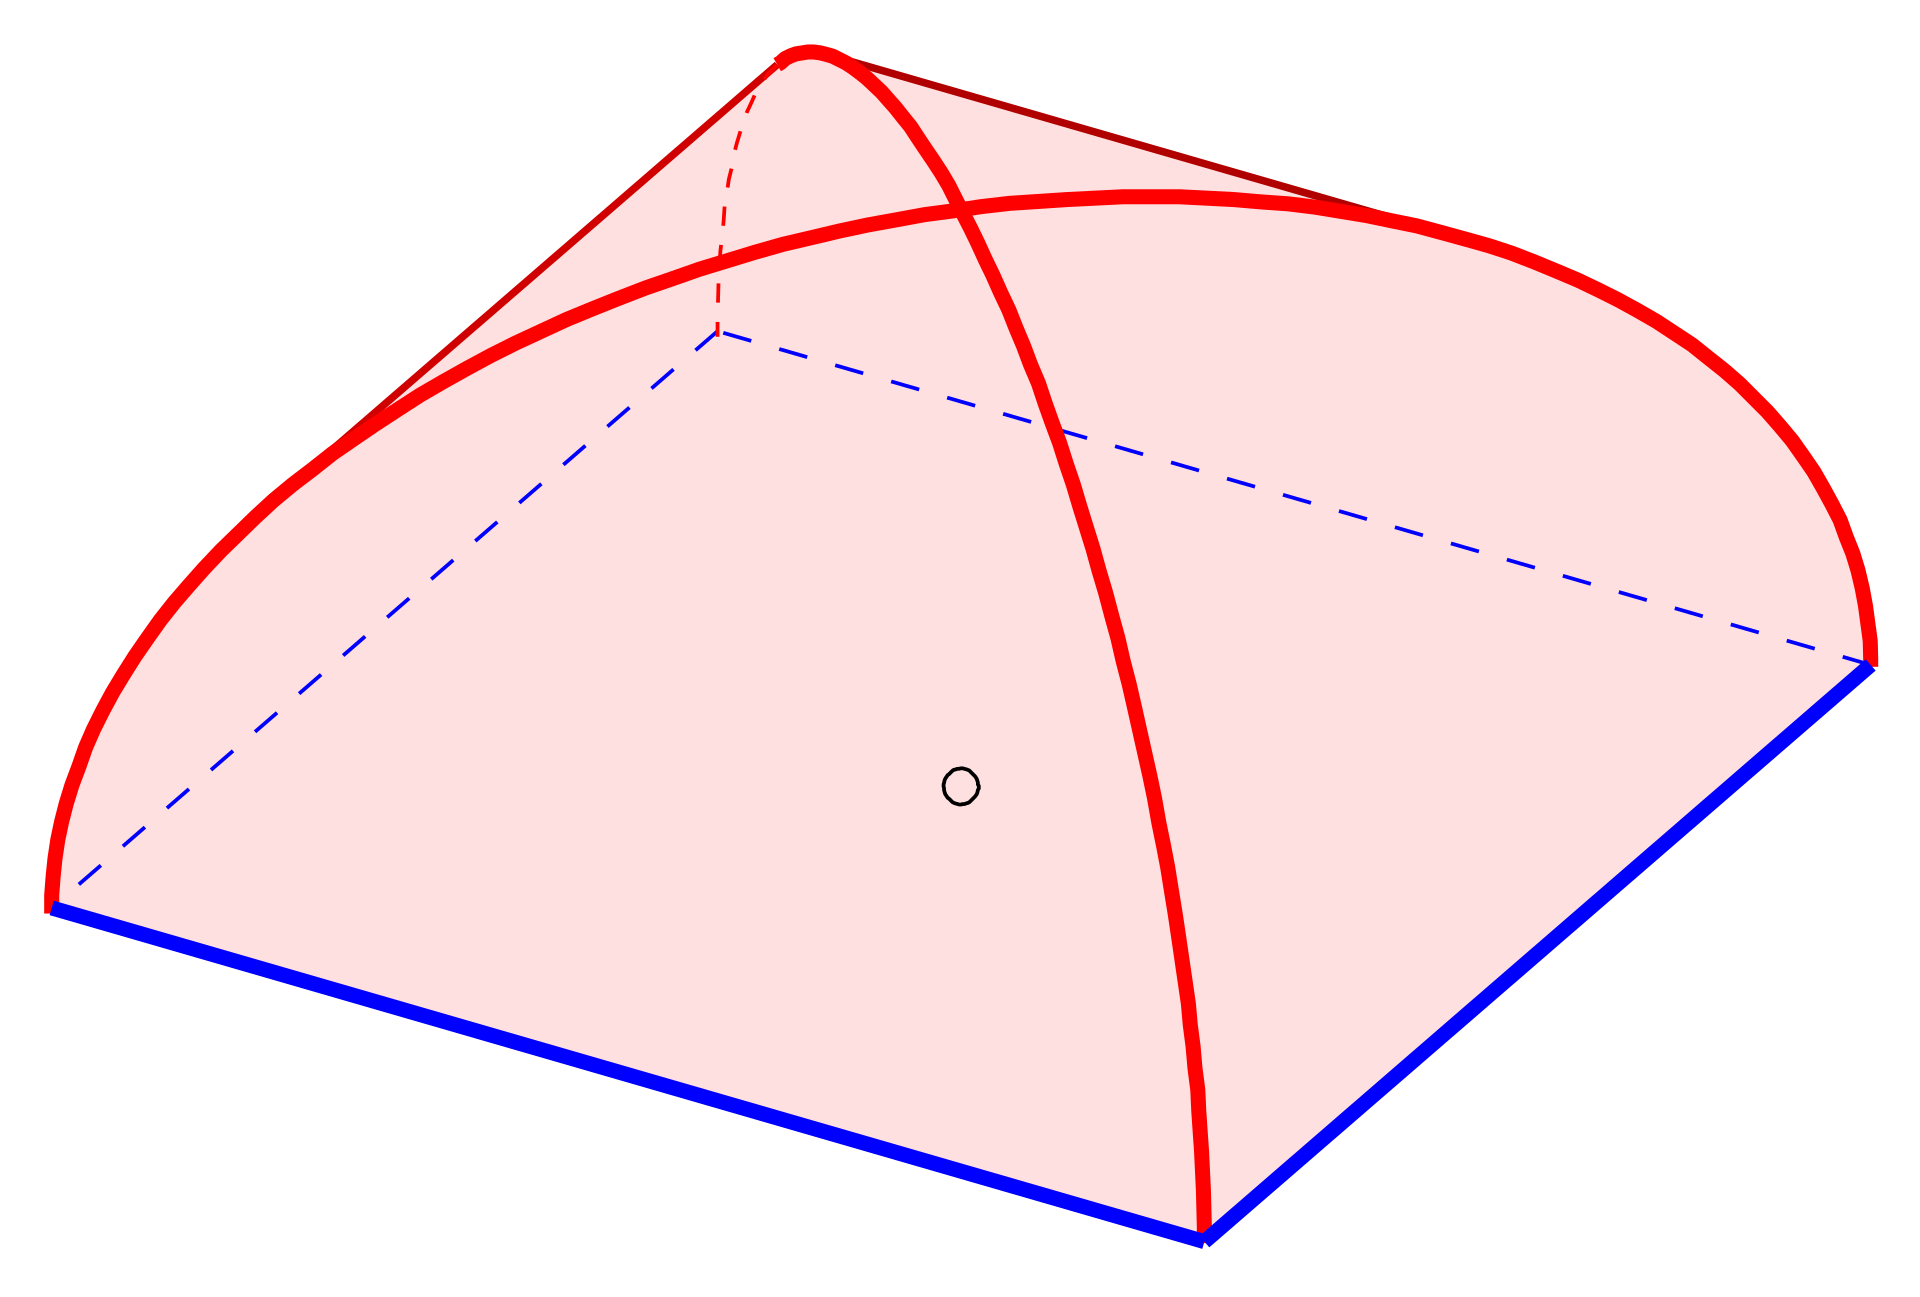
\includegraphics[scale=0.06]{Klostergew.png} 
\end{minipage}
\begin{minipage}{0.75\textwidth}
\vspace{4mm}
\begin{ex} Consideriamo un vassoio da pasticceria determinato dai punti $(x,y,z)$ dello spazio che soddisfano $z\geq 0, x^2+z^2\leq 1, y^2+z^2\leq 1$ (ossia l'intersezione tra due cilindri con assi ortogonali e il semispazio delle $z$ non negative). Qual è il suo volume? 
\end{ex}
\textbf{Soluzione}. È semplice osservare che per qualunque $z\in[0,1)$ la sezione orizzontale è un 
\end{minipage}
quadrato di area $4(1-z^2)$. Dal principio di Cavalieri segue pertanto che il volume cercato è $4\int_{0}^{1}(1-z^2)\,dz$, ossia $\color{blue}\frac{8}{3}$.

\begin{center}
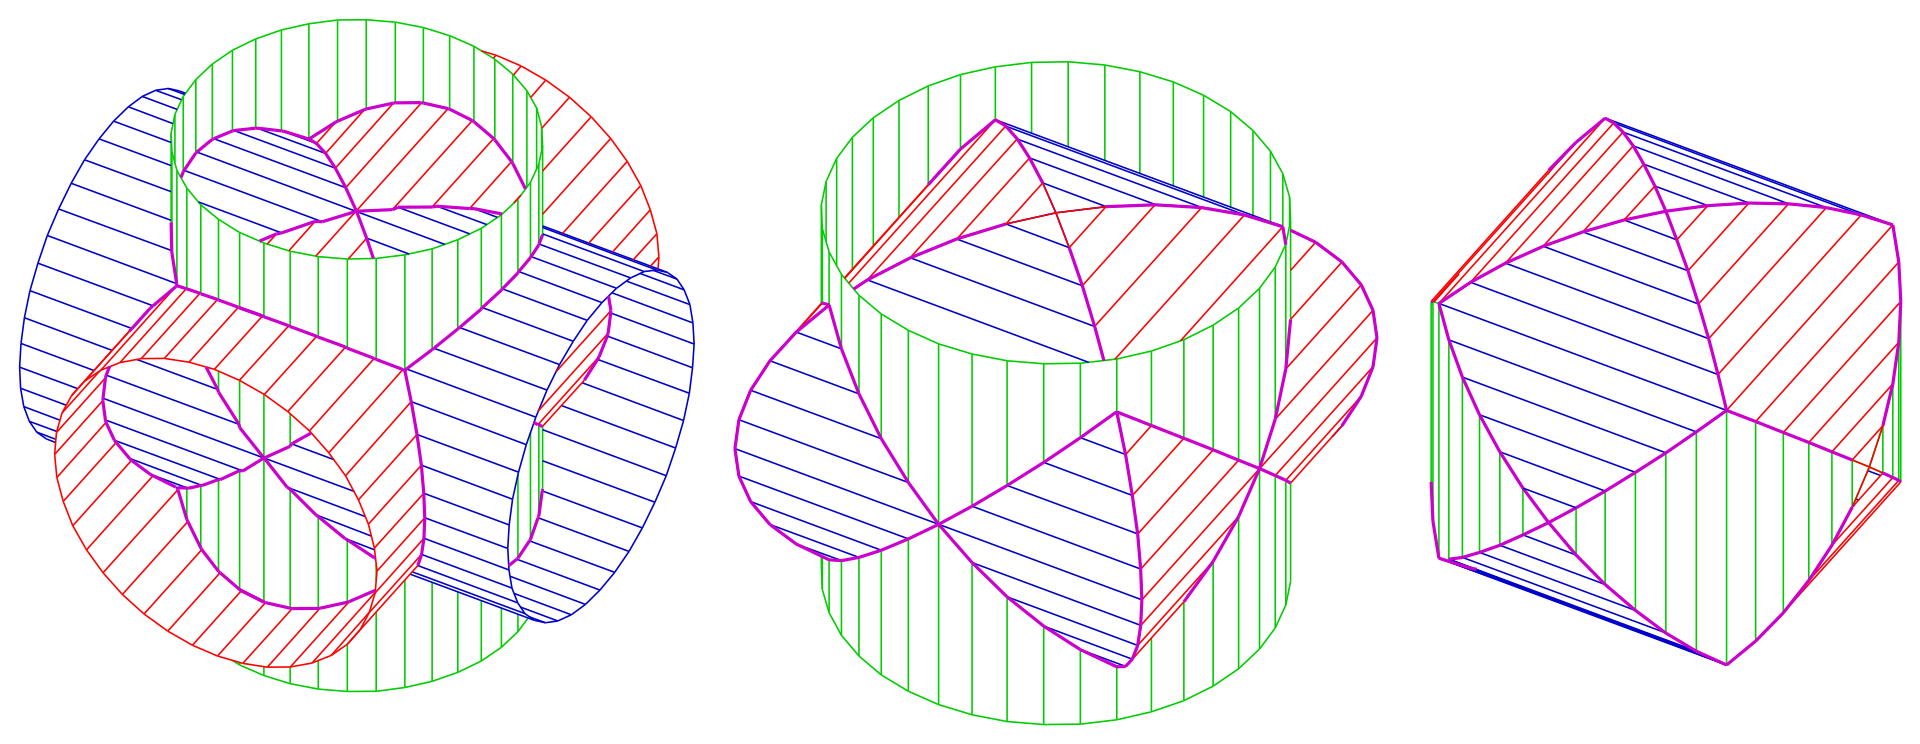
\includegraphics[scale=0.18]{Steinmetz.png} 
\end{center}
\begin{ex} Consideriamo ora il \emph{solido di Steinmetz} determinato dall'intersezione di \emph{tre} cilindri\\ con assi mutuamente ortogonali, $\{(x,y,z)\in\R^3: x^2+y^2\leq 1, y^2+z^2\leq 1, z^2+x^2\leq 1\}.$ 
Quanto vale il volume?  
\end{ex}
\textbf{Soluzione}. Procedendo come prima abbiamo che la sezione relativa a un certo $z\in(-1,1)$ è quadrata se $|z|\in\left[\frac{1}{\sqrt{2}},1\right]$ ed ha la forma dell'intersezione tra un quadrato ed un cerchio se $|z|<\frac{1}{\sqrt{2}}$. Da una raffigurazione accurata possiamo anche intuire che il solido è decomponibile nell'unione tre un cubo di spigolo $\sqrt{2}$ e $6$ cupole, ognuna delle quali con volume dato da $\int_{1/\sqrt{2}}^{1}4(1-z^2)\,dz=\frac{8-5\sqrt{2}}{3}$. Segue che il volume del solido di Steinmetz è $\color{blue}8(2-\sqrt{2})$: quasi il $12\%$ in più del volume della sfera inscritta, che ha esattamente le stesse proiezioni sui piani coordinati.

\begin{ex} Si provi che la superficie del precedente solido di Steinmetz è $24(2-\sqrt{2})$.
 
\end{ex}


\newpage

\section{Successioni per ricorrenza}
Lo studio di successioni in cui il termine generale $a_n$ dipende in qualche modo dai precedenti è di fondamentale importanza non solo dal punto di vista strettamente teorico, ma anche da quello fisico-ingegneristico, visto che è piuttosto raro essere in grado di ricostruire esplicitamente la soluzione di un'equazione differenziale, ma si hanno migliori chances di successo nella trattazione (eventualmente numerica) dei corrispondenti problemi \emph{linearizzati} o altrimenti \emph{discretizzati}. Il primo caso che ci apprestiamo a trattare è quello delle successioni per ricorrenza \emph{lineari} ed \emph{autonome}, dove il termine generale $a_n$ è una fissata combinazione lineare dei precedenti $k$ termini.

\subsection{Successione di Fibonacci e similia}
Un problema prototipico è quello di determinare una formula esplicita (\emph{formula di Binet}) per la successione (\emph{di Fibonacci}) $\{F_n\}_{n\geq 0}$ definita dalle \emph{condizioni iniziali} $F_0=0, F_1=1$ e dalla (legge di) \emph{ricorrenza} $F_{n+2}=F_{n+1}+F_n$, valida per ogni $n\in\N$. Illustriamo diversi approcci equivalenti.\\

\textbf{Approccio \#1, \emph{rasoio di Occam}}. L'insieme delle successioni $\{a_n\}_{n\geq 0}$ che soddisfano la ricorrenza $a_{n+2}=a_{n+1}+a_n$ è uno \emph{spazio vettoriale}. In uno slancio di ottimismo, cerchiamo elementi ragionevolmente \emph{semplici} di questo spazio vettoriale, ossia \emph{successioni di potenze} $a_n=\alpha^n$ che rispettano la ricorrenza.
Imporre che si abbia $a_{n+2}=a_{n+1}+a_n$ è equivalente ad imporre che la quantità $\alpha$ soddisfi $\alpha^2=\alpha+1$, ossia risulti radice del \emph{polinomio caratteristico} $p(x)=x^2-x-1$. Per quanto noto dall'antichità più remota sulle proporzioni del pentagono regolare, le radici del precedente polinomio sono il \emph{rapporto aureo} $\varphi=\frac{1+\sqrt{5}}{2}$ e il suo coniugato algebrico $\overline{\varphi}=\frac{1-\sqrt{5}}{2}$. In virtù della struttura di spazio vettoriale, \emph{tutte} le successioni della forma $a_n = A\varphi^n + B\overline{\varphi}^n$ soddisfano la ricorrenza voluta. Nell'ultima espressione abbiamo due gradi di libertà nella scelta dei coefficienti $A,B$, ed auspicabilmente un'opportuna scelta della coppia $(A,B)$ è tale da garantire simultaneamente sia $a_0=F_0=0$ che $a_1=F_1=1$, ossia 
$$ \left\{\begin{array}{rcl}\varphi^0 A + \overline{\varphi}^0 B &=& 0 \\ \varphi^1 A + \overline{\varphi}^1 B &=& 1.\end{array}\right. $$
In virtù della regola di Cramer il sistema ha effettivamente soluzione unica, poiché 
$$ \det \begin{pmatrix} 1 & 1 \\ \varphi & \overline{\varphi} \end{pmatrix}=\overline{\varphi}-\varphi \neq 0, $$
caso particolare del fatto che tutte le matrici di Vandermonde definite a partire da elementi distinti sono invertibili.\\
A conti fatti abbiamo $A=-B=\frac{1}{\sqrt{5}}$, dunque la successione $a_n=\frac{\varphi^n-\overline{\varphi}^n}{\sqrt{5}}$ rispetta sia la legge di ricorrenza che le condizioni iniziali volute. Dal principio di induzione segue pertanto $a_n=F_n$, ossia 
$$ F_n = \frac{\varphi^n-\overline{\varphi}^n}{\sqrt{5}}. $$

\textbf{Approccio \#2, \emph{Jordan}}. Possiamo liberamente definire il vettore $v_n=\begin{pmatrix} F_{n+1} \\ F_{n}\end{pmatrix}$ ed esprimere la ricorrenza nella forma $v_{n+1} = M v_n$, dove $M=\begin{pmatrix} 1 & 1 \\ 1 & 0\end{pmatrix}$. Dal principio di induzione segue $v_n = M^n v_0$, dunque il problema di esplicitare il termine generale della successione si rivela equivalente a quello di esplicitare l'$n$-esima potenza della matrice $M$. Dal Teorema di Jordan si ha $M = J^{-1}\begin{pmatrix}\varphi & 0 \\ 0 & \overline{\varphi}\end{pmatrix} J$ per un'opportuna matrice invertibile $J$, da cui $M^n = J^{-1}\begin{pmatrix}\varphi^n & 0 \\ 0 & \overline{\varphi}^n\end{pmatrix} J$. Segue che il termine generale della successione è una fissata combinazione lineare di $\varphi^n$ e $\overline{\varphi}^n$, dove i coefficienti di questa combinazione lineare possono essere facilmente calcolati per interpolazione, o (meno efficientemente) esplicitando la matrice $J$.\\

\textbf{Approccio \#3, \emph{OGF}}. Questo è un approccio estremamente potente, ma decisamente indiretto: associamo alla successione una funzione regolare, dalla ricorrenza deduciamo proprietà algebriche della funzione, dalle ultime ricostruiamo il comportamento esplicito (o anche solo asintotico) della successione. È immediato realizzare che la successione di Fibonacci è crescente, ma non troppo rapidamente, in quanto si ha $a_{n+1}\leq 2 a_n$ per ogni $n\geq 1$, da cui $F_n \leq 2^{n-1}$.\\ In particolare, posto 
$$ f(x) = \sum_{n\geq 0} F_n x^n  = x + \sum_{n\geq 2}F_n x^n$$
si ha che $f(x)$ è una funzione analitica in un intorno circolare dell'origine di raggio almeno $\frac{1}{2}$.\\ Su questo insieme abbiamo 

$$ x^2 f(x) = \sum_{n\geq 0} F_n x^{n+2} = \sum_{n\geq 2} F_{n-2} x^n,\qquad x f(x) = \sum_{n\geq 0} F_n x^{n+1} = \sum_{n\geq 2} F_{n-1} x^n $$
e dalla relazione $F_{n}=F_{n-1}+F_{n-2}$, valida per ogni $n\geq 2$, deduciamo che 
$$ f(x) = x + x f(x) + x^2 f(x)\quad\Longrightarrow\quad f(x) = \frac{x}{1-x-x^2}. $$
Operando una decomposizione in fratti semplici dell'ultima funzione razionale, mediante serie geometriche otteniamo che 
$$ f(x) = \frac{1}{\sqrt{5}}\left(\frac{1}{1-\varphi x}-\frac{1}{1-\overline{\varphi}x}\right) = \frac{1}{\sqrt{5}}\sum_{n\geq 0}\left(\varphi^n-\overline{\varphi}^n\right) x^n. $$
Dal principio di identità delle funzioni analitiche (diretta estensione del principio di identità dei polinomi: se due funzioni analitiche coincidono in un intorno dell'origine hanno le medesime derivate in zero e viceversa) segue la formula di Binet. $f(x)$ è detta \emph{funzione generatrice ordinaria (OGF)} della successione $\{F_n\}_{n\geq 0}$ e l'effettivo raggio di convergenza nell'origine è dato dal reciproco del massimo modulo delle radici del polinomio caratteristico (Teorema di Frobenius), nel nostro caso $\frac{1}{\varphi}=\varphi-1\approx 0.618$.\\

Gli ultimi due approcci sono immediatamente generalizzabili al caso in cui una successione per ricorrenza lineare ed autonoma abbia ordine $k\geq 2$. Il primo approccio è praticabile solo se le radici del polinomio caratteristico sono tutte distinte: altrimenti si manifestano problemi di \emph{risonanza}, legati alle potenze di una matrice non diagonalizzabile, o ai \emph{poli} di funzioni razionali con ordine maggiore di $1$. Vediamone un esempio.

\begin{ex} La successione $\{a_n\}_{n\geq 0}$ è definita dalla condizioni iniziali $a_0=1, a_1=2, a_2=5$ e dalla ricorrenza $a_{n+3}=3 a_{n+2}-4 a_n$, valida per ogni $n\in\N$. Si determini un'espressione esplicita del termine generale. 
\end{ex}

\textbf{Soluzione}. Il polinomio caratteristico della ricorrenza è $p(x)=x^3-3x^2+4=(x-2)^2(x+1)$, dunque le successioni $b_n=2^n$ e $c_n=(-1)^n$ soddisfano la ricorrenza. Due elementi non sono sufficienti a generare uno spazio vettoriale di dimensione $3$, ma il ``terzo escluso'' può essere facilmente determinato considerando che la matrice compagna del polinomio $p(x)$ è simile a 
$$\begin{pmatrix} 2 & 1 & 0 \\ 0 & 2 & 0 \\ 0 & 0 & -1\end{pmatrix}, $$
dunque lo spazio vettoriale è generato da $2^n, n 2^n$ e $(-1)^n$ e $a_n = A 2^n + B n 2^n + C(-1)^n$ con 
$$\left\{\begin{array}{rcl}A+C&=& 1 \\ 2A+2B-C&=& 2 \\ 4A+8B+C&=&5\end{array}\right. $$
che conduce a $A=\frac{8}{9}$, $B=\frac{1}{6}$, $C=\frac{1}{9}$.\qed

\begin{ex}[Tribonacci] In funzione di $n\in\N^+$ si determini il numero $T_n$ di stringhe binarie di lunghezza $n$ all'interno delle quali non sono mai presenti tre caratteri $1$ consecutivi. Si determini infine una buona approssimazione numerica del limite $\lim_{n\to +\infty}\sqrt[n]{T_n}$.
\end{ex}

\begin{ex} Si determini una forma esplicita per il termine generale di $\{a_n\}_{n\geq 1}$, dove $a_1=\frac{\sqrt{3}}{2}$ e $a_{n+1}=\sqrt{\frac{1+a_n}{2}}$ per ogni $n\geq 1$.
\end{ex}
\textbf{Soluzione}. Abbiamo in questo caso una successione autonoma, in cui la ricorrenza è intimamente legata alla formula di bisezione del coseno. Posto $a_n=\cos(\theta_n)$ abbiamo infatti $\theta_1=\frac{\pi}{6}$ e $a_{n+1}=\cos\left(\frac{\theta_n}{2}\right)$, da cui facilmente $a_n=\cos\left(\frac{\pi}{3\cdot 2^n}\right)$.

\begin{ex} Si determini una forma esplicita per il termine generale di $\{a_n\}_{n\geq 1}$, dove $a_1=\frac{1}{2}$ e $a_{n+1}=2a_n^2-1$ per ogni $n\geq 1$.
\end{ex}
\textbf{Soluzione}. Con la stessa sostituzione utilizzata nell'esercizio precedente, possiamo osservare in questo caso una manifestazione della formula di duplicazione del coseno, che comporta $a_n=\cos\left(\frac{\pi}{6}2^n\right)$ e il fatto che la successione sia definitivamente periodica (in questo caso, addirittura, costante dal secondo termine in poi).

\subsection{Successioni non autonome}
Nel caso di successioni per ricorrenza \emph{non} autonome è molto raro che si riesca a determinare una formula esplicita per il termine generale. È tuttavia importante conoscere almeno qualche caso in cui ciò \emph{è} possibile: ad esempio situazioni in cui, mediante sostituzioni opportune, ci si può ricondurre alla risoluzione di una ricorrenza autonoma.

\begin{ex} Si determini una forma esplicita per il termine generale di $\{a_n\}_{n\geq 1}$, dove $a_1=1$ e $a_{n+1}=n\cdot a_n$\\ per ogni $n\geq 1$. 
\end{ex}
\textbf{Soluzione}. La ricorrenza può essere espressa come $\frac{a_{n+1}}{a_n}=n$, dove il membro sinistro è il termine generale di un prodotto telescopico. In particolare
$$ \frac{a_{N+1}}{a_1}=\prod_{n=1}^{N}\frac{a_{n+1}}{a_n} = \prod_{n=1}^{N}n = N!$$
conduce immediatamente a $a_n = (n-1)!$.

\begin{ex} Si determini una forma esplicita per il termine generale di $\{a_n\}_{n\geq 1}$, dove $a_1=1$ e $a_{n+1}=n\cdot a_n + 1$ per ogni $n\geq 1$.
\end{ex}
\textbf{Soluzione}. Visto e considerato l'esercizio precedente, poniamo $a_n=(n-1)! b_n$ e osserviamo che per la successione $\{b_n\}_{n\geq 1}$ abbiamo di conseguenza $b_1=1$ e $n!\cdot b_{n+1} = n!\cdot b_n + 1$, ossia $b_{n+1}-b_n=\frac{1}{n!}$. Il membro sinistro dell'ultima equazione è il termine generale di una somma telescopica, da cui 
$$ b_{N+1}-b_1 = \sum_{n=1}^{N}\left(b_{n+1}-b_n\right) = \sum_{n=1}^{N}\frac{1}{n!}$$
e di conseguenza $b_{N+1}=\sum_{n=0}^{N}\frac{1}{n!}$, così come $a_n = (n-1)!\sum_{k=0}^{n-1}\frac{1}{k!}$. 
Questo esercizio è strettamente legato al conteggio delle \emph{dismutazioni} in $S_n$, ossia permutazioni senza punti fissi.\\


Più in generale si può cercare di tradurre (e risolvere) una ricorrenza lineare ma non omogenea in una equazione algebrica o differenziale per la funzione generatrice ordinaria (OGF) $\sum a_n z^n$ o per la funzione generatrice esponenziale (EGF) $\sum \frac{a_n}{n!} z^n$. Un caso celebre è dato dalla successione $\{C_n\}_{n\geq 0}$ con $C_0=1$ e $C_n=\sum_{k=1}^{n}C_{k-1}C_{n-k}$, che enumera certi percorsi sotto-diagonali in una griglia quadrata. In questo caso (numeri \emph{di Catalan}) si ha $C_n=\frac{1}{n+1}\binom{2n}{n}$ da semplici manipolazioni applicate alla serie di Maclaurin di $\sqrt{1-z}$. Per approfondimenti rimandiamo al Wilf o al Flajolet.


\section{Equazioni differenziali}
Esistono fenomeni in cui rapidità di variazione di una certa quantità è proporzionale (o comunque legata algebricamente), in ogni istante, alla quantità stessa.
Gli esempi più tipici di sono ottenuti spesso e volentieri dalla Fisica, e la loro complessità varia in maniera drammatica in base al contesto. Esempi degni di nota verranno fatti nel paragrafo apposito.

\subsection{Teorema di Cauchy-Lipschitz}
Il più importante risultato sull'esistenza e l'unicità delle soluzioni di equazioni differenziali è il seguente.
\begin{theo}[Cauchy-Lipschitz] Dato il \emph{problema di Cauchy}
$$\left\{\begin{array}{rcl}y'(t) &=& f(t,y(t)) \\ y(0)&=&y_0 \end{array}\right. $$
con $f$ funzione continua nel primo argomento (il tempo) e lipschitziana nel secondo argomento (la $y$),\\ allora il problema ammette soluzione unica in un intorno dell'origine. 
\end{theo}
\textbf{Idea della dimostrazione}. La prima condizione può essere espressa come $y(x)=y_0+\int_{0}^{x}f(t,y(t))\,dt$. Possiamo dunque considerare un operatore (di Volterra) $T$ che manda una generica $g$, continua in un intorno dell'origine, in 
$$ (T g)(x) = y_0 + \int_{0}^{x} f(t,g(t))\,dt $$
ed applicare il metodo di punto fisso che consiste nel definire una successione di funzioni $y_0(x)=y_0, y_n(x)=Ty_n(x)$, sperabilmente convergente all'unica soluzione del problema di Cauchy. I tecnicismi della dimostrazione sono finalizzati a provare che, nelle ipotesi su $f$, l'operatore di Volterra è effettivamente una contrazione, il che permette di concludere invocando il Teorema di Banach-Caccioppoli.  
\begin{proof} Definiamo preliminarmente un intorno chiuso di $(0,y_0)$ costituito dai $(t,g(t))$ per cui $|t|\leq A$\\ e $\|g-y_0\|_{\infty}\leq B$, con $A$ e $B$ costanti positive. Su questo intorno possiamo assumere di avere $|f|\leq M$\\ e che $f$ sia $L$-lipschitziana rispetto alla seconda variabile. Osserviamo che 
$$ \left|(Tg)(x)-y_0\right|=\left|\int_{0}^{x}f(t,g(t))\,dt\right| \leq \int_{0}^{x}\left|f(t,g(t))\right|\,dt \leq M|x| $$
dunque a meno di rimpiazzare $A$ con $\min\left(A,\frac{B}{M}\right)$ abbiamo che l'operatore $T$ manda elementi dell'intorno iniziale in elementi dell'intorno iniziale. Osserviamo poi che 
$$\left|(Tg_1)(x)-(Tg_2)(x)\right|=\left|\int_{0}^{x}f(t,g_1(t))-f(t,g_2(t))\,dt\right| \leq \int_{0}^{x}L|g_1(t)-g_2(t)|\,dt \leq L|x|\cdot\|g_1-g_2\|_{\infty}$$
dunque a meno di rimpiazzare $A$ con $\min\left(A,\frac{1}{L}\right)$ abbiamo che $T$ è una contrazione debole sull'intorno di partenza.\\
Da Banach-Caccioppoli segue che l'operatore $T$ ha un unico punto fisso, dato ad esempio dal limite puntuale della successione definita attraverso $y_0(t)=y_0$ e $y_{n+1}(t)=(Ty_n)(t)$. Poiché i punti fissi dell'operatore di Volterra sono esattamente le soluzioni del problema di Cauchy, il Teorema è dimostrato.
\end{proof}

\textbf{Nota \#1}: riguardo l'intervallo massimale su cui è unicamente definita la soluzione, possiamo rimuovere la dipendenza da $L$ osservando che 
$$ \left\| T^m \varphi_1(t)- T^m\varphi_2(t)\right\|_{\infty}\leq \frac{L^m|t|^m}{m!}\|\varphi_1-\varphi_2\|_{\infty} $$
per ogni $t$ tale che $|t|\leq\min\left(A,\frac{B}{M}\right)$. Vista la rapidità con cui cresce il fattoriale, il membro destro è sicuramente dominato da $\|\varphi_1-\varphi_2\|_{\infty} $ per qualche $m\in\N$. In particolare possiamo replicare la precedente dimostrazione rimpiazzando l'operatore $T$ con $T^m$, ottendendo che l'intervallo massimale di esistenza e unicità delle soluzioni dipende unicamente dall'insieme di definizione del campo $f$ e dal massimo modulo del campo $f$, ma non dalla sua costante di Lipschitz.\\

\textbf{Nota \#2}: concatenando tra loro più istanze di esistenza e unicità \emph{in piccolo} possiamo in molti casi provare la \emph{globalità} di una soluzione. Se ad esempio il campo $f$ è sublineare rispetto alla seconda variabile, è automatico che le soluzioni del problema di Cauchy siano globali: questo ad esempio comporta che tutte le soluzioni di ED lineari omogenee a coefficienti costanti siano globali\footnote{In verità questo è palese anche come conseguenza del metodo di Frobenius, che accennerremo più avanti: le soluzioni delle ED lineari omogenee a coefficienti costanti sono funzioni intere di ordine $1$, ben più che $C^{\infty}$ e globali.}. Ovviamente non è vero il viceversa, ma il Teorema di Okamura fornisce sia condizioni sufficienti che necessarie per l'esistenza e unicità della soluzione di un problema di Cauchy: fondamentalmente, l'esistenza di un'opportuna funzione di Lyapunov.

\begin{ex} Si determinino le soluzioni del problema di Cauchy
$$\left\{\begin{array}{rcl}u'(t)&=&\sqrt{u(t)}\\ u(0)&=&\alpha    \end{array}\right. $$
al variare di $\alpha$ in $[0,+\infty)$.
\end{ex}
\textbf{Soluzione}. Abbiamo in questo caso che il campo $f(x)=\sqrt{x}$ è continuo sul suo dominio, ma non è differenziabile nell'origine. Integrando sul generico intervallo $[0,T]$ (con $T>0$) ambo i membri di 
$$ \frac{u'(t)}{\sqrt{u(t)}} = 1 $$
otteniamo 
$$ 2\left(\sqrt{u(T)}-\sqrt{\alpha}\right) = T $$
da cui $u(T)=\left(\frac{T}{2}+\sqrt{\alpha}\right)^2$. D'altra parte è chiaro che quest'ultima non possa essere una soluzione per tutti i tempi, inclusi quelli negativi: laddove è definita una qualunque soluzione del problema di Cauchy è non-negativa e debolmente crescente. Studiando il problema nel passato (ossia su $[-T,0]$ con $T>0$) abbiamo che la soluzione generale per $\alpha>0$ è data da 
$$ u(t) = \left\{\begin{array}{rcl}\left(\frac{t}{2}+\sqrt{\alpha}\right)^2 &\text{se}& t\geq -2\sqrt{\alpha} \\ 0 & \text{se} & t\leq -2\sqrt{\alpha}. \end{array}\right. $$
Nel caso $\alpha=0$ viene a mancare l'unicità della soluzione, in quanto sia la funzione costantemente nulla che la precedente soluzione con $\alpha=0$ risultano risolvere il problema di partenza.



\subsection{Classificazione delle principali equazioni differenziali}
Per il Teorema Fondamentale del Calcolo Integrale (TFCI), sotto opportune ipotesi di regolarità possiamo ricostruire $u(t)$ dalla sua derivata $u'(t)$ e dal valore di $u$ in un punto. L'equazione $u'(t)=f(t)$ ha infatti soluzione $$u(t)=\int_{a}^{t}f(s)\,ds.$$
In generale, data una funzione di due variabili $f(t,u)$ possiamo porci il problema di trovare una funzione $u(t)$ che verifichi l'equazione differenziale:$$u'(t)=f(t,u(t)).$$
L'equazione di sopra si dice del primo ordine perché coinvolge solo la derivata prima della funzione $u(t)$.
\subsubsection{ED a variabili separabili}
Si chiamano così le equazioni del tipo: $$u'(t)=a(t)f(u(t)).$$ 
Per risolvere queste equazioni basta dividere entrambi i membri per $f(u)$ ed integrare: $$\int\frac{u'(t)}{f(u(t))}\,dt=\int a(t)\,dt.$$
In particolare, posto di saper determinare esplicitamente la primitiva di $a$ e  l'inversa della primitiva di $\frac{1}{f}$\\ (condizione talvolta piuttosto gravosa), questi problemi sono di semplice risoluzione.

\begin{ex} Si determini una soluzione di $f'(t)=f(t)^2+1$ che soddisfa $f(0)=1$, e il più grande intorno dell'origine su cui questa soluzione risulta continua. 
\end{ex}
\textbf{Soluzione}. Possiamo osservare che, posto che $f$ sia definita, $f(t)^2+1\geq 1$, dunque ogni soluzione è continua e crescente in un intorno dell'origine e su tale intorno $f$ risulta invertibile. Integrando ambo i membri di $\frac{f'(t)}{f(t)^2+1}=1$ sul generico intervallo $[0,\alpha]$ otteniamo $\arctan(f(\alpha))-\arctan(f(0))=\alpha$, equivalente a $\arctan(f(\alpha))=\alpha+\frac{\pi}{4}$ e a
$$ f(\alpha)=\tan\left(\alpha+\frac{\pi}{4}\right)=\frac{1+\tan(\alpha)}{1-\tan(\alpha)},$$
il cui intorno massimale di iniettività è dato da $\left(-\frac{3\pi}{4},\frac{\pi}{4}\right)$.

\begin{ex} Si determini l'intervallo di esistenza della soluzione di $f'(t)=f(t)^2+f(t)$ che soddisfa $f(0)=1$. 
\end{ex}
\textbf{Soluzione}. Con l'idea di procedere come nel caso precedente, procuriamoci dapprima una primitiva di $\frac{1}{u^2+u}$.\\ Per decomposizione in fratti semplici 
$$ \int \frac{du}{u^2+u} = \int\left(\frac{1}{u}-\frac{1}{u+1}\right)\,du = \log(u)-\log(u+1) = -\log\left(1+\frac{1}{u}\right), $$
per cui integrando ambo i membri di $\frac{f'(t)}{f(t)^2+f(t)}=1$ sul generico intervallo $[0,\alpha]$ abbiamo $\log(2)-\log\left(1+\frac{1}{f(\alpha)}\right)=\alpha$, equivalente a $1+\frac{1}{f(\alpha)}=\exp\left(\log 2-\alpha\right)$ e a $\frac{1}{f(\alpha)}=-1+2 e^{-\alpha}$, da cui 
$$ f(\alpha) = \frac{e^{\alpha}}{2-e^{\alpha}}. $$
Segue che l'intervallo di esistenza della soluzione è dato da $(-\infty,\log 2)$.

\subsubsection{ED lineari del primo ordine}
Sono le equazioni del tipo: $$u'(t)=a(t)u(t)+b(t)$$
con $a(t)$ e $b(t)$ funzioni date.
\subsubsection{Equazioni lineari omogenee del primo ordine}
\begin{theorem}
    Sia $I$ intervallo di $\R$, sia $a:I \to \R$ una funzione continua; e siano $t_0\in I$ e $y_0\in\R$ fissati.\\ Esiste un'unica funzione $\phi\in C^1$ tale che 
    $$\phi'(t)=a(t)\phi(t)\qquad \text{ per ogni } t\in I,\phi(t_0)=y_0$$
    Questa $\phi$ è data dalla formula: 
    $$\phi(t) =y_0\cdot \exp\left(\int_{t_0}^{t_1}a(s)\,ds\right).$$
\end{theorem}
\begin{proof}
    È immediato verificare che la formula definita sopra soddisfa $\phi(t_0)=y_0$, e $\phi'(t)=\exp\left(\int_{t_0}^{t}a(s)\, ds\right)\phi(t)$, per il teorema di Torricelli. Per verificare l'unicità supponiamo che sia $\psi'(t)-a(t)\psi(t)=0$ identiticamente in $I$, poiché $t\to \exp\left(-\int_{t_0}^{t}a(s)\, ds\right)$ non è mai nulla, si ha:
    $$\psi'(t)-a(t)\psi(t)=0\Leftrightarrow \exp\left(-\int_{t_0}^{t}a(s)\, ds\right)(\psi'(t)-a(t)\psi(t))=0$$
    Si osservi ora che
    $$e^{-\int_{t_0}^{t}a(s)\, ds}\psi'(t)-e^{-\int_{t_0}^{t}a(s)\, ds}a(t)\psi(t)=\frac{d}{dt}\left(e^{-\int_{t_0}^{t}a(s)\, ds}\psi(t)\right)$$
    La relazione precedente si scrive come
    $$\psi'(t)-a(t)\psi(t)=0\Leftrightarrow \frac{d}{dt}\left(e^{-\int_{t_0}^{t}a(s)\, ds}\psi(t)\right)=0$$
    poiché una funzione ha derivata nulla in un intervallo solo se è costante deve valere
    $$\psi'(t)-a(t)\psi(t)=0\Leftrightarrow e^{-\int_{t_0}^{t}a(s)\, ds}\psi(t)=c$$
    con $c\in\R$ costante. per $t=t_0$ si ha che $e^{-\int_{t_0}^{t}a(s)ds}\psi(t_0)=\psi(t_0)$ e quindi $c=\psi(t_0)$.
\end{proof}
\begin{cor}
    Se $I$ è un intervallo di $\R$ ed $a:I\to\R$ è continua, tutte le soluzioni della differenziale $$y'=a(t)y$$
    sono definite dalla formula:
    $$y(t)=ce^{A(t)}$$
    al variare di $c\in\R$, con $A(t)$ primitiva di $a(t)$ su $I$.
\end{cor}


\subsubsection{ED lineari non omogenee del primo ordine}
Lo stesso metodo porta alla risoluzione delle equazioni differenziali lineari non omogenee di grado 1.
\begin{theorem}
    Il problema
    $$y'=a(t)y+b(t)\quad y(t_0)=y_0$$
    con $a,b:I\to\R$ funzioni continue e $t_0\in I$ ammette come unica soluzione
    $$y(t)=y_0e^{\int_{t_0}^{t}a(s)\, ds}+ e^{\int_{t_0}^{t}a(s)\, ds}\int_{t_0}^{t}e^{-\int_{t_0}^{s}a(\sigma)\, d\sigma}\,b(s) ds.$$ 
\end{theorem}

Non è difficile verificare che l'ultima funzione è effettivamente soluzione dell'ED $y'=a(t)\,y+b(t)$, e che questa è unica in virtù del Teorema di Cauchy-Lipschitz. Tuttavia è preferibile padroneggiare l'\emph{idea} che permette di ricondurre un'equazione differenziale non omogenea ad una omogenea, che è semplicemente quella di utilizzare opportune sostituzioni. Se poniamo $y(t)=M(t)f(t)$ abbiamo 
$$y'(t)=M'(t)f(t)+M(t)f'(t)=a(t)M(t)f(t)+b(t)$$
e possiamo scegliere $M(t)$ in modo che si abbia $M'(t)=a(t)M(t)$, in modo da ricondurre il problema alla risoluzione di $M(t)f'(t)=b(t)$, che è a variabili separabili. A meno di traslazioni dell'argomento possiamo inoltre sempre assumere, senza perdita di generalità, che si abbia $t_0=0$. Vediamo un esempio esplicito.
\begin{ex} Si determini la soluzione di $y'(t) = t\cdot y(t)+t^2$ che soddisfa $y(1)=1$. 
\end{ex}
\textbf{Soluzione}. Poniamo da subito $y(t)=f(t-1)$, in modo da ricondurci al problema 
$$ f'(t) = (t+1) f(t)+(t+1)^2,\qquad f(0)=1.$$
Una soluzione di $M'(t)=(t+1)M(t)$ è data da $\exp\left(\frac{t^2}{2}+t\right)$: poniamo dunque $f(t)=\exp\left(-\frac{t^2}{2}-t\right)g(t)$ e osserviamo che questa sostituzione ci permette di ricondurci alla risoluzione di 
$$ (t+1)\exp\left(\frac{t^2}{2}+t\right)g(t) + \exp\left(\frac{t^2}{2}+t\right)g'(t) = (t+1)\exp\left(\frac{t^2}{2}+t\right)g(t)+(t+1)^2,\qquad g(0)=1,$$
ossia alla risoluzione di 
$$  g'(t) = (t+1)^2 \exp\left(-t-\frac{t^2}{2}\right),\qquad g(0)=1,$$
che fornisce $g(t)=1+\int_{0}^{t}(s+1)^2 \exp\left(-s-\frac{s^2}{2}\right)\,ds$. In questo caso $g$ non ha un'espressione chiusa in termini di funzioni elementari (dipende dalla funzione $\operatorname{Erf}$, ossia dai quantili della distribuzione normale), ma al di là di questo è certo che si abbia 
$$f(t) = \exp\left(\frac{t^2}{2}+t\right)+\exp\left(\frac{t^2}{2}+t\right)\int_{0}^{t}(s+1)^2 \exp\left(-s-\frac{s^2}{2}\right)\,ds$$
e $y(t)=f(t-1)$.

\begin{ex} Si determinino le soluzioni dell'equazione differenziale 
$$ \dot{x}(t) = \frac{x(t)}{t}+\frac{t}{2x(t)}.$$
\end{ex}
\textbf{Soluzione}. Ponendo $x(t) = t\cdot z(t)$ abbiamo $\dot{x} = z+t\dot{z}$ e 
$$ z + t\dot{z} = z+\frac{1}{2z} $$
che è equivalente a $2\dot{z}z = \frac{1}{t}$. Integrando ambo i membri sul generico intervallo $(0,T)$ con $T>0$ otteniamo\\ $z^2(T)-z^2(0)=\log(T)$, da cui $x(t)=t\cdot \sqrt{z(0)^2+\log t}$.

\subsubsection{ED lineari ordinarie a coefficienti costanti}
Un caso di grande interesse teorico e pratico è quello delle equazioni differenziali in cui una combinazione lineare, a coefficienti costanti, di $f(x)$ e di una quantità finita di sue derivate coincida con zero (caso omogeneo) o con una funzione assegnata (caso non omogeneo). Vedremo più avanti (nella sezione \emph{Trasformata di Laplace}) che la risoluzione del problema di ordine $n$
$$ f(x) + c_1 f'(x) + \ldots + c_n f^{(n)}(x) = 0$$
è di fatto equivalente alla determinazione della forma esplicita di una successione per ricorrenza, lineare ed autonoma, di ordine $n$. Se $n=1$ abbiamo una ED a variabili separabili. Più in generale ($n\geq 2$) possiamo osservare che, posto d'ufficio $u(x)=\left(f(x),f'(x),\ldots,f^{(n-1)}(x)\right)\in\R^{n-1}$, il precedente problema può essere espresso come 
$$ u'(x) = M\,u(x) $$
dove $M$ è la \textbf{matrice compagna} del \textbf{polinomio caratteristico}
$$ p(\lambda) = c_n \lambda^n + \ldots + c_1 \lambda + 1. $$
In analogia con il caso scalare, la soluzione di $u'(x)=M\,u(x)$ è determinata dall'esponenziale di $M$, definito come la serie $1+M+\frac{M^2}{2!}+\frac{M^3}{3!}+\ldots$. Dall'Algebra Lineare (forma normale di Jordan) abbiamo che $M$ è coniugata ad una matrice triangolare superiore avente sulla diagonale gli autovalori di $M$, ossia le radici (potenzialmente complesse) del polinomio $p(\lambda)$, contate con molteplicità. Il Teorema di Cayley-Hamilton comporta allora che $e^M$ sia coniugata ad una matrice triangolare superiore, che ha sulla diagonale gli esponenziali delle radici di $p(\lambda)$. Nel caso in cui $p(\lambda)$ abbia radici distinte (ovvero discriminante non nullo) è automatico che $M$ sia diagonalizzabile, dunque che la soluzione generale sia della forma 
$$ f(x) = \kappa_1 e^{\lambda_1 x}+\ldots+\kappa_n e^{\lambda_n x}, $$
con $\lambda_1,\ldots,\lambda_n$ radici del polinomio caratteristico e $\kappa_1,\ldots,\kappa_n$ scalari fissati dalle condizioni iniziali.\\
Le soluzioni dell'equazione omogenea restano uno spazio vettoriale di dimensione $n$ anche nel caso in cui $M$ non sia diagonalizzabile, ma se $p(\lambda)$ ha una radice $\eta$ di molteplicità $k\geq 2$, questa contribuisce alla soluzione attraverso i termini $\kappa_1 e^{\eta x}+\kappa_2 x e^{\eta x}+\ldots+\kappa_{k-1} x^{k-1} e^{\eta x}$, dunque la soluzione generale diviene una combinazione lineare non di soli esponenziali, ma di esponenziali moltiplicati per opportuni monomi. Quest'ultimo fatto può essere dimostrato considerando la struttura delle potenze di un generico blocco di Jordan o, forse più agevolmente, attraverso la trasformata di Laplace, come vedremo più avanti.

\subsection{Esempi}
\subsubsection{Decadimento radioattivo}
È il processo secondo il quale un sostanza radioattiva decade, trasformandosi in un'altra sostanza più leggera a causa della perdita di neutroni. Indicando con $n(t)$ il numero di neutroni presenti al tempo $t$, il modello prevede che durante l'istante $dt$ una percentuale $p$ fissata di $n(t)$ decada, dando luogo all'equazione

$$ n(t+dt)-n(t) = -p\cdot n(t)\, dt\quad\Leftrightarrow\quad n'(t) = -p\cdot n(t) $$ 

che è una ED a variabile separabili, con soluzione data da 

$$ n(t) = n(0)\cdot e^{-pt}. $$

Si ha in particolare che durante ogni intervallo di durata $\tau=\frac{\log 2}{p}$ il numero di neutroni presenti nella sostanza si dimezza. Pertanto $\tau$ è detto \emph{tempo di dimezzamento}.

\subsubsection{Problemi di Gravitazione}

Il più semplice problema di Gravitazione è quello in cui si suppone che un punto materiale, inizialmente fermo e a distanza $H$ dal suolo, cada verso il suolo per effetto di una accelerazione di modulo $g$ costante. Nel sistema di riferimento in cui la posizione $x=0$ corrisponde al suolo, il problema è dunque descritto da 
$$ \ddot{x}=-g,\qquad \dot x = -gt,\qquad x(t) = H-\frac{1}{2}gt^2 $$
e il tempo di caduta $T$ è dato dalla soluzione positiva di $x(t)=0$, ossia $T=\sqrt{\frac{2H}{g}}$.\\
Alla medesima conclusione si può pervenire osservando che nell'ultima situazione, così come in tutti i problemi di cinematica in cui intervengono solo forze conservative, una certa funzione delle variabili $x$ e $\dot{x}$ (che determinano il \emph{piano delle fasi}) è costante nel tempo. Considerata infatti $f(x,\dot{x})=2g x+\dot{x}^2$ abbiamo 
$$ \dot{f} = 2g\dot{x} + 2\dot{x}\ddot{x} = 2\dot{x}(g+\ddot{x}) = 0. $$
Ciò fornisce un legame esplicito tra la posizione del punto materiale e la sua velocità: in corrispondenza di una qualunque posizione $x\in[0,H]$ la velocità del punto materiale è $\dot{x}=-\sqrt{2g(H-x)}$. Questa corrispondenza può essere espressa anche come $\frac{dx}{dt}=-\sqrt{2g(H-x)}$, e il Teorema della funzione implicita/inversa assicura la validità della seguente manipolazione algebrica dell'ultima identità:
$$ \frac{dx}{\sqrt{2g(H-x)}} = -dt. $$
Integrando ambo i membri dell'ultima identità tra la posizione iniziale e quella finale abbiamo che 
$$ T = \frac{1}{\sqrt{2g}}\int_{0}^{H}\frac{dx}{\sqrt{H-x}}\stackrel{x\mapsto Hz}{=}\frac{H}{\sqrt{2g}}\int_{0}^{1}\frac{dz}{\sqrt{H}\sqrt{1-z}}\stackrel{z\mapsto 1-z}{=}\sqrt{\frac{H}{2g}}\int_{0}^{1}\frac{dz}{\sqrt{z}}\stackrel{z\mapsto u^2}{=}\sqrt{\frac{H}{2g}}\int_{0}^{1}2\,du = \sqrt{\frac{2H}{g}}. $$
Nel caso di accelerazione costante l'ultimo approccio per la determinazione di $T$ è evidentemente meno efficiente rispetto alla semplice risoluzione di un'equazione di secondo grado, ma ha il pregio di essere incredibilmente più generale. Se infatti affrontiamo il problema della caduta di un grave dove l'accelerazione risponde alla legge di gravitazione universale, nelle stesse ipotesi di inizio sezione abbiamo 
$$ \ddot{x} = -\frac{g}{\left(1+\frac{x}{R}\right)^2} $$
dove $R$ indica il raggio terrestre. Normalizzando le lunghezze in base a quest'ultimo possiamo ricondurci all'equazione differenziale $\ddot{x} = -\frac{c}{(1+x)^2}$, e in questo caso è evidente quanto \emph{non sia} immediato dedurre la legge oraria. È comunque piuttosto semplice ricavare l'espressione esplicita di $\dot{x}(t)$: come in tutti i casi in cui $\ddot{x}=g(x)$ possiamo osservare che si ha
$$ 2\dot{x}\ddot{x} = -2c\frac{\dot{x}}{(1+x)^2}\quad\Longleftrightarrow\quad \frac{d}{dt}\dot{x}^2 = 2c\cdot\frac{d}{dt}\left(\frac{1}{1+x}\right) $$
dunque $\dot{x}^2-\frac{2c}{1+x}$ (che è il rapporto tra il doppio dell'\textbf{energia meccanica} del punto materiale e la massa del punto materiale) non varia nel tempo, restando pari a $-\frac{2c}{1+x(0)}$. Di nuovo, ciò comporta un legame tra posizione e velocità (ossia il fatto che il moto sia descritto da una specifica curva nel piano delle fasi):
$$ \dot{x}^2 = 2c\left(\frac{1}{1+x}-\frac{1}{1+x(0)}\right). $$
E di nuovo, dall'ultima equazione possiamo dedurre come varia il tempo al variare della posizione:
$$ \frac{dt}{dx} = -\frac{1}{\sqrt{2c}}\left(\frac{1}{1+x}-\frac{1}{1+x(0)}\right)^{-1/2}. $$
Integrando ambo i membri tra la posizione iniziale $x(0)>1$ e la posizione finale $x(T)=1$ abbiamo 
$$ T = \frac{1}{\sqrt{2c}}\int_{1}^{x(0)}\left(\frac{1}{1+x}-\frac{1}{1+x(0)}\right)^{-1/2}\,dx=\frac{1}{\sqrt{2g}}\int_{0}^{H}\left(\frac{1}{1+\frac{x}{R}}-\frac{1}{1+\frac{H}{R}}\right)^{-1/2}\,dx,$$
$$T=\sqrt{\frac{R+H}{2g}}\left(\sqrt{\frac{H}{R}}+\left(1+\frac{H}{R}\right)\arctan\sqrt{\frac{H}{R}}\right). $$
Per altezze iniziali inferiori al raggio terrestre abbiamo
$$T\approx \sqrt{\frac{R+H}{2g}}\left(2\left(\frac{H}{R}\right)^{1/2}+\left(\frac{H}{R}\right)^{3/2}\right) $$
che al primo ordine è $1+\frac{H}{2R}$ volte il tempo di caduta in presenza di accelerazione costante.

\subsubsection{Moto in presenza di attrito viscoso}
Un altro problema interessante è quello della caduta di un grave in presenza di accelerazione costante, ma anche di attrito viscoso, forza dissipativa di intensità direttamente proporzionale alla velocità. Nel riferimento in cui ${x(0)=H>0}$ e $\dot{x}(0)=0$ l'equazione differenziale che regola il moto è dunque 
$$ \ddot{x} = -g-\eta \dot{x}, $$
ED lineare ordinaria di ordine $2$, che attraverso la sostituzione $y=\dot{x}+\eta x$ è ricondotta ad una equazione a variabili separabili, $\dot{y}=-g$, che comporta $y=-\eta H-gt$ e 
$$ \dot{x}-\eta x = \eta H -gt, $$
ED lineare del primo ordine a coefficienti costanti, non omogenea, che ha per soluzione 
$$ x(t) = H + \frac{g}{\eta^2}\left(1-\eta t-e^{-\eta t}\right),\qquad \dot{x}(t)=-\frac{g}{\eta}\left(1-e^{-\eta t}\right). $$
In questa situazione fisica il modulo della velocità non può superare la velocità limite $\frac{g}{\eta}$ e il tempo di caduta è dato dalla soluzione di un'equazione trascendente, esplicitabile mediante la funzione di Lambert $W$ (inversa di $xe^x$).

\subsubsection{Oscillatore armonico}
Con questo termine si indica un sistema costituito da un punto materiale di massa $m$ che si muove su una retta, soggetto ad una forza di richiamo, la cui intensità è proporzionale alla distanza dall'origine. \\
Indicando con $x(t)$ la posizione del corpo al tempo $t$, l'equazione differenziale che regola il moto è
$$ m\ddot{x} + k x = 0 $$
con $m$ e $k$ scalari positivi. Questa è una ED lineare, omogenea, a coefficienti costanti di ordine $2$, con polinomio caratteristico $p(\lambda)=m\lambda^2+k$. Le radici del polinomio caratteristico sono $\pm i\sqrt{\frac{k}{m}}$, dunque la soluzione generale è data da una combinazione lineare di $\sin\left(\sqrt{\frac{k}{m}}\,t\right)$ e $\cos\left(\sqrt{\frac{k}{m}}\,t\right)$, ossia è della forma 
$$ x(t) = A \cos\left(\varphi_0 + \omega t\right) $$
dove la pulsazione $\omega$ corrisponde a $\sqrt{\frac{k}{m}}$. In particolare ogni soluzione è periodica di periodo $\frac{2\pi}{\omega} = 2\pi\sqrt{\frac{m}{k}}$, come prevedibile anche dal fatto che le orbite nel piano delle fasi sono ellissi centrate nell'origine:
$$ 2m\dot{x}\ddot{x} + 2k x \dot{x}=0\quad\Longrightarrow\quad \frac{d}{dt}\left(m\dot{x}^2+k x^2\right) = 0\quad \Longrightarrow\quad \dot{x}^2+(\omega x)^2=\text{costante}.$$





\subsubsection{Pendolo fisico}
Supponiamo che un punto materiale di massa $m$ sia vincolato all'estremità libera di un'asta rigida di lunghezza $\ell$, supponiamo che l'asta abbia massa trascurabile e abbia l'altra estremità incerneriata nel punto del piano di coordinate $(0,\ell)$. Se nella configurazione iniziale l'asta determina un angolo $\theta_0\in[0,\pi/2]$ con la verticale, la conservazione dell'energia meccanica conduce all'equazione differenziale 
$$ \frac{m}{2}\left(\ell\dot{\theta}\right)^2 + mg\ell(1-\cos\theta) = mg\ell(1-\cos\theta_0) $$
equivalente a 
$$ \dot{\theta}^2  = \frac{2g}{\ell}(\cos\theta-\cos\theta_0) $$
che comporta
$$ \dot{\theta}+\frac{g}{\ell}\sin\theta = 0. $$
Nell'assunzione che l'angolo iniziale $\theta_0$ sia sufficientemente piccolo è dunque sensato aspettarsi che il sistema si evolva in maniera analoga a quello determinato da $\dot{\theta}+\frac{g}{\ell}\theta = 0$, ossia un oscillatore armonico di periodo $2\pi\sqrt{\frac{\ell}{g}}$, indipendente da $\theta_0$ (isocronia del pendolo per le piccole oscillazioni). Senza rimpiazzare il potenziale con la sua approssimazione al second'ordine possiamo comunque osservare che 
$$ \left|\frac{dt}{d\theta}\right| = \sqrt{\frac{\ell}{2g}}\cdot\frac{1}{\sqrt{\cos\theta-\cos\theta_0}} $$
dunque per simmetria il periodo esatto è dato da 
$$ T = \sqrt{\frac{\ell}{2g}}\cdot 4\int_{0}^{\theta_0}\frac{d\theta}{\sqrt{\cos\theta-\cos\theta_0}}=4\sqrt{\frac{\ell}{g}}\int_{0}^{\pi/2}\frac{d\varphi}{\sqrt{1-\sin^2\frac{\theta_0}{2}\sin^2\varphi}}. $$
L'ultimo integrale è un \emph{integrale ellittico completo del primo tipo}. Per quanto dimostrato da Gauss questi oggetti sono direttamente collegati alla \emph{media aritmo-geometrica ($\operatorname{AGM}$)}. Per il pendolo fisico vale in particolare che 
$$ T = \frac{2\pi\sqrt{\frac{\ell}{g}}}{\operatorname{AGM}\left(1,\cos\frac{\theta_0}{2}\right)}\in 2\pi\sqrt{\frac{\ell}{g}}\left(\frac{2}{1+\cos\frac{\theta_0}{2}},\frac{1}{\sqrt{\cos\frac{\theta_0}{2}}}\right). $$
Troncando al second'ordine, la dipendenza del periodo dall'angolo iniziale è della forma $T\approx 2\pi\sqrt{\frac{\ell}{g}}\left(1+\frac{\theta_0^2}{16}\right).$\\
Se l'angolo iniziale è esattamente $\frac{\pi}{2}$, a causa di valori speciali dell'integrale ellittico completo del primo tipo\\ si ha esattamente $T=\Gamma^2\left(\frac{1}{4}\right)\sqrt{\frac{\pi\ell}{4g}}$, cioè circa $\frac{13}{7}$ del periodo delle piccole oscillazioni.

\subsection{Metodi di risoluzione di ED lineari non omogenee}

Considerando che le soluzioni di 
$$ f(t) + c_1(t) f'(t) + \ldots + c_n(t) f^{(n)}(t) = 0 $$
formano uno spazio vettoriale, le soluzioni di 
$$ f(t) + c_1(t) f'(t) + \ldots + c_n(t) f^{(n)}(t) = g(t) $$
costituiscono uno spazio affine, dunque ogni soluzione dell'ultima ED è data dalla somma tra una soluzione particolare di $ f(t) + c_1(t) f'(t) + \ldots + c_n(t) f^{(n)}(t) = g(t) $ e una combinazione lineare delle soluzioni dell'equazione omogenea. Nel caso (piuttosto comune) in cui $g(t)$ sia una combinazione lineare di termini della forma $t^n e^{\lambda t}$ (con $n\in\N$ e $\lambda\in\C$), una tecnica per determinare una soluzione particolare è il \textbf{metodo di somiglianza}, che consiste nel ricercare soluzioni $f(t)$ che abbiano la stessa ``struttura algebrica'' di $g(t)$.\footnote{L'\emph{handwaving} di questa sezione è rimosso dalla sezione successiva.} Nella risoluzione di  
$$ u'(t)+2u(t) = t^2$$
cerchiamo ad esempio soluzioni particolari che siano polinomi. Per come l'operatore di derivazione agisce sullo spazio dei polinomi (ossia riducendo di $1$ il grado dei polinomi non costanti) possiamo assumere senza perdita di generalità che una soluzione particolare sia della forma $at^3+bt^2+ct+d$.  Derivando otteniamo $u'(t)=3at^2+2bt+c$: utilizzando la relazione data dalla differenziale e risolvendo un semplice sistema lineare otteniamo che $p(t)=\frac{1}{4}(2t^2-2t+1)$ è soluzione particolare.
La soluzione generale è quindi $u(t)= p(t) + c_1 e^{-2t}$.\\
Un altro metodo per risolvere alcune differenziali (più complesse delle precedenti) 
è quello di ricorrere ad opportune sostituzioni, della variabile indipendente o della funzione obiettivo, ad esempio considerando l'equazione differenziale soddisfatta dalla funzione inversa di una soluzione (si vedano a tal proposito le \textbf{condizioni di Osgood}).\\

\begin{ex} Si determinino le soluzione dell'equazione differenziale 
$$ \dot{x}+\frac{x}{t+1} = 6t. $$
\end{ex}
\textbf{Soluzione}. Ponendo $x(t)=(t+1)f(t)$ ci riduciamo a risolvere 
$$ (t+1)f'(t) + 2f(t) = 6t, $$
ponendo $f(t)=g(t)+2t$ ci riduciamo a risolvere 
$$ (t+1) g'(t) + 2g(t)  = -2 $$
e ponendo $g(t)=-1+h(t)$ ci riduciamo a risolvere l'omogenea
$$ (t+1)h'(t)+2h(t) = 0 $$
che è a variabili separabili. Da $\frac{h'(t)}{h(t)}=-\frac{2}{t+1}$ abbiamo $\log h(T)-\log h(0)=-2\log(1+T)$ e $h(t)=\frac{C}{(1+t)^2}$,\\ da cui $x(t)=\frac{2t^3+3t^2+C}{t+1}$.\\

Un altro metodo di riferimento per le ED lineari non omogenee è il \textbf{metodo di variazione delle costanti}.

\begin{ex} Si determinino le soluzioni dell'equazione differenziale 
$$ \ddot{x}+x = \frac{1}{\cos t}. $$
\end{ex}
\textbf{Soluzione}. Osserviamo che l'equazione omogenea è quella di un oscillatore armonico, con soluzione generale data da $A\cos t+B\sin t$. In analogia a quanto fatto per risolvere le ED lineari non omogenee del prim'ordine, cerchiamo soluzioni della forma $A(t)\cos t+B(t)\sin t$, rimpiazzando appunto le costanti che figurano nella soluzione generale dell'omogenea con funzioni inizialmente incognite. Con questa sostituzione si ha 
$$ \dot{x}(t) = B(t)\cos(t)-A(t)\sin(t)+A'(t)\cos(t)+B'(t)\sin(t)$$
e se imponiamo che valga $A'(t)\cos(t)+B'(t)\sin(t)=0$ abbiamo che l'equazione di partenza è equivalente a 
$$ B'(t)\cos(t)-A'(t)\sin(t) = \frac{1}{\cos t}.$$
Risolvendo un sistema lineare otteniamo $A'(t)=-\tan t$ e $B'(t)=1$, da cui la soluzione generale 
$$ x(t) = (A+\log|\cos t|)\cos(t) + (B+t)\sin t.$$




\newpage

\subsection{Trasformata di Laplace}
La trasformata di Laplace è uno strumento essenziale in Teoria dei Numeri, Teoria dei Controlli, Probabilità e Analisi Armonica. È un operatore lineare definito come segue: data $f:\R^+\to\R$, la sua trasformata di Laplace $\mathcal{L}f:\R^+\to \R$ è data da
$$ (\mathcal{L} f)(s) = \int_{0}^{+\infty} f(x) e^{-sx}\,dx. $$
La questione riguardo il dominio massimale dell'operatore $\mathcal{L}$ e la corrispondente immagine è affrontata e risolta dai Teoremi di Schwartz e Paley-Wiener, ma per i nostri scopi è sufficiente restringere l'indagine alle funzioni $f:\R^+\to\R^+$ continue e tali per cui $f(x)e^{-sx}$ sia impropriamente Riemann-integrabile su $\R^+$ per ogni $s>0$. Su questo spazio di partenza non è difficile provare che l'operatore $\mathcal{L}$ è iniettivo, e che inoltre gode di interessanti proprietà algebriche, tra cui:
\begin{itemize}
 \item $\mathcal{L}$ trasforma equazioni differenziali lineari ordinarie a coefficienti costanti in equazioni algebriche, poiché per integrazione per parti si ha che la trasformata di Laplace di $f^{(n)}(x)$ è la somma tra un polinomio di grado $(n-1)$ della variabile $s$ e $s^n\cdot(\mathcal{L}f)(s)$;
 \item $\mathcal{L}$ è un operatore autoaggiunto, ossia $\int_{0}^{+\infty}f(x)\cdot(\mathcal{L}g)(x)\,dx = \int_{0}^{+\infty}(\mathcal{L} f)(x)\cdot g(x)\,dx.$ (Per Fubini) 
\end{itemize}
Tramite integrazione per parti non è difficile procurarsi la trasformata di Laplace della generica soluzione di una ED lineare ordinaria a coefficienti costanti:
$$ \mathcal{L}\left( x^n e^{-\lambda x} \right)(s) = \frac{n!}{(\lambda+s)^{n+1}}$$
e l'ultima identità, interpretata ``alla rovescia'', fornisce anche l'anti-trasformata di Laplace di qualunque funzione razionale che sia decomponibile in fratti semplici\footnote{E in verità anche qualcosa in più, visto che $n$ non è strettamente vincolato ad essere un naturale.}. Vediamone subito un'applicazione, anche per chiarire quanto anticipato nei paragrafi precedenti.
\begin{ex} Si determini la soluzione dell'equazione differenziale 
$$ f''(x)-2f'(x)+f(x)=\sin(x) $$
che soddisfa $f(0)=1$ e $f'(0)=0$.
\end{ex}
\textbf{Soluzione}. Applicando $\mathcal{L}$ ad ambo i membri dell'ED in questione\footnote{Legittimo in quanto la limitatezza del seno assicura che le soluzioni dell'equazione differenziale rientrino a pieno titolo nel dominio ristretto di $\mathcal{L}$ che abbiamo considerato a inizio sezione.} otteniamo 

$$ (s-1)^2\cdot(\mathcal{L}f)(s)+(2-s) = \frac{1}{1+s^2} $$
che ci fornisce immediatamente ed esplicitamente la trasformata di Laplace della soluzione:
$$ (\mathcal{L}f)(s) = \frac{1}{(s^2+1)(s-1)^2}+\frac{s-2}{(s-1)^2}. $$
Il membro destro è una funzione razionale con un polo doppio in $s=1$ e poli semplici in $s=\pm i$.\\ Applicando una decomposizione in fratti semplici e successivamente $\mathcal{L}^{-1}$ concludiamo che 
$$ f(x) = \frac{\cos(x)+(1-x)e^x}{2}. $$
\\
Vediamo anche un'altra applicazione uber-celebre.
\begin{ex}[Integrale di Dirichlet] Si determini esplicitamente il valore dell'integrale di Riemann improprio $$\int_{0}^{+\infty}\frac{\sin x}{x}\,dx.$$
\end{ex}
\textbf{Soluzione}. L'integrale è finito per il criterio di Abel-Dirichlet: $\sin x$ ha primitiva limitata e $\frac{1}{x}$ è decrescente a zero su $\R^+$. Possiamo inoltre osservare che $\frac{1}{s}$ è la trasformata di Laplace della funzione che vale identicamente $1$. Dall'auto-aggiunzione della trasformata di Laplace segue allora che 
$$ \int_{0}^{+\infty}\frac{\sin x}{x}\,dx = \int_{0}^{+\infty}\sin(s)\cdot(\mathcal{L} 1)(s)\,ds = \int_{0}^{+\infty}(\mathcal{L}\sin(x))(s)\cdot 1\,ds = \int_{0}^{+\infty}\frac{ds}{1+s^2}={\color{blue}\frac{\pi}{2}}. $$

\textbf{Nota}: la tecnica appena implementata è anche più potente di quanto possa sembrare a prima vista. Nel caso di integrali calcolabili mediante applicazione del Teorema dei residui (Cauchy) l'auto-aggiunzione della trasformata di Laplace permette spesso di giungere alle medesime conclusioni senza la necessità di dare la caccia a opportuni circuiti di integrazione nel piano complesso.\\

\begin{ex}[Integrali di Frullani] Si determini esplicitamente il valore dell'integrale di Riemann improprio 
$$ \int_{0}^{+\infty}\frac{e^{-2x}-e^{-3x}}{x}\,dx.$$ 
\end{ex}
\textbf{Soluzione}. Osservando come prima che $\frac{1}{x}$ è la trasformata di Laplace della funzione che vale costantemente $1$ abbiamo 
$$ \int_{0}^{+\infty}\frac{e^{-2x}-e^{-3x}}{x}\,dx = \int_{0}^{+\infty}\mathcal{L}(e^{-2x}-e^{-3x})(s)\,ds = \int_{0}^{+\infty}\left(\frac{1}{s+2}-\frac{1}{s+3}\right)\,ds=\left[\log\left(\frac{s+2}{s+3}\right)\right]_{0}^{+\infty}={\color{blue}\log\left(\frac{3}{2}\right)}. $$
Equivalentemente, da Fubini 

$$ \int_{0}^{+\infty}\frac{e^{-2x}-e^{-3x}}{x}\,dx \stackrel{x\mapsto -\log u}{=}\int_{0}^{1}\frac{u^2-u}{\log u}\,du=\int_{0}^{1}\int_{1}^{2}u^\alpha\,d\alpha\,du = \int_{1}^{2}\int_{0}^{1}u^\alpha\,du\,d\alpha = \int_{1}^{2}\frac{d\alpha}{\alpha+1}=\left[\log(\alpha+1)\right]_{1}^{2}. $$

Un'ulteriore applicazione della trasformata di Laplace è la determinazione puntuale di serie di Fourier.
\begin{ex}[\emph{Sawtooth wave}] Si determini il limite per $x\to 0^+$ della funzione $f(x)$ definita da
$$ f(x) = \sum_{n\geq 1}\frac{\sin(nx)}{n}. $$
\end{ex}
\textbf{Soluzione}. Per sommazione per parti $f(x)$ è limitata e periodica, ma non è detto che sia continua.\\ In ogni caso la limitatezza comporta che 
$$ \lim_{x\to 0^+}f(x) = \lim_{s\to +\infty}\int_{0}^{+\infty}f(x)\cdot s e^{-sx}\,dx = \lim_{s\to +\infty} s\cdot(\mathcal{L} f)(s). $$
Dalla linearità di $\mathcal{L}$ si ha che 
$$ s\cdot(\mathcal{L}f)(s) = \sum_{n\geq 1}\frac{s}{n^2+s^2} = \frac{-1+\pi s\coth(\pi s)}{2s},$$
da cui $\lim_{x\to 0^+}f(x)=\frac{\pi}{2}$, che conferma il sospetto sulla non-continuità di $f$.\\

Evidenziamo infine come i seguenti tre problemi siano di fatto equivalenti:
\begin{itemize}
 \item soluzione di una ED lineare a coefficienti costanti 
 \item soluzione di una equazione per ricorrenza lineare ed autonoma
 \item determinazione delle potenze o dell'esponenziale di una matrice.
\end{itemize}

Data infatti una ricorrenza della forma 
$$ a_{n+k} = c_1 a_{n+k-1} + c_2 a_{n+k-2} + \ldots + c_k a_n $$
possiamo definire il vettore colonna 
$$ v_n = \left(a_{n+k-1},a_{n+k-2},\ldots,a_n\right)^t $$
ed esprimere la ricorrenza come 
$$ v_{n+1} = \begin{pmatrix}c_1 & c_2 & c_3 & \ldots & c_k \\ 
                            1 & 0 & 0 &\ldots & 0 \\
                            0 & 1 & 0 &\ldots & 0 \\
                            0 & 0 & \ddots & \ldots & 0 \\
                            0 & 0 & \ldots & 1 & 0\end{pmatrix} v_n = M v_n $$
da cui segue, per induzione, $v_n = M^n v_0$. Il polinomio caratteristico di $M$ è esattamente lo stesso del polinomio caratteristico della ricorrenza: $M$ è infatti coniugata alla matrice che rappresenta la moltiplicazione per $x$ nell'anello quoziente $\R[x]/(p(x))$, dove $p(x)=x^k-c_1 x^{k-1}-\ldots-c_k$. Segue che il termine generale $a_n$ è fissato da $M^n$, ed è dunque combinazione lineare di termini della forma $n^j \lambda^n$ con $\lambda$ autovalore di $M$ (ossia radice di $p$) e $j$ che varia da $0$ fino alla molteplicità algebrica di $\lambda$ diminuita di $1$. D'altra parte la ricorrenza può essere interpretata come un'equazione differenziale. Posto infatti $f(x)=\sum_{n\geq 0}\frac{a_n}{n!}x^n$, ossia considerata la funzione generatrice esponenziale della successione $\{a_n\}_{n\geq 0}$, si ha quanto segue:
$$ [x^n]f^{(k)}(x) = [x^n]\frac{d^k}{dx^k}\sum_{n\geq k}\frac{a_n}{n!}x^n=[x^n]\sum_{n\geq k}\frac{a_n}{(n-k)!}x^{n-k}=\frac{a_{n+k}}{n!}$$
per cui la ricorrenza risulta equivalente alla ED
$$ f^{(k)}(x) = c_1 f^{(k-1)}(x) + c_2 f^{(k-1)}(x) + \ldots + c_k f(x) $$
e passando in trasformata 
$$ s^k (\mathcal{L}f)(s) = \left(c_1 s^{k-1}+\ldots c_k\right)(\mathcal{L}f)(s)+Q(s) $$
con $Q(s)$ polinomio di grado $\leq (k-1)$ che dipende unicamente dalle condizioni iniziali (ossia da $v_0$).\\
Da semplici manipolazioni algebriche segue 
$$ f(x) = \mathcal{L}^{-1}\left(\frac{Q(s)}{s^k-c_1 s^{k-1}-\ldots-c_k}\right)(x) $$
e la decomposizione in fratti semplici dell'ultima funzione razionale entro parentesi chiude il circolo di equivalenze.

\subsection{Accenno al metodo di Frobenius}
Abbiamo visto che le ED della forma $u'(t)=f(t)u(t)$ sono tutte facilmente risolubili, e possiamo chiederci se lo stesso valga per le ED della forma $u''(t)=f(t)u(t)$.
\begin{shaded}\begin{ex}[Funzioni di Airy] Si determini il comportamento su $\R$ e un'espressione esplicita per la soluzione dell'equazione differenziale 
$$ f''(x) = x\cdot f(x) $$
che soddisfa $f(0)=1$ e $f'(0)=0$. \end{ex}
\end{shaded}
\textbf{Soluzione}. Ancora prima di giungere ad una espressione esplicita per la soluzione, osserviamo che il comportamento di questa a destra e a sinistra dell'origine è radicalmente diverso. Preso un valore di $M\in\R^+$ sufficientemente grande, il comportamento della soluzione sull'intervallo $[M,M+1]$ è analogo al comportamento della soluzione di $g''(x)=M g(x)$ che soddisfa $g(M)=f(M)$ e $g'(M)=f'(M)$, ossia una funzione positiva, convessa e crescente che in $M+1$ vale approssimativamente $f(M)\exp(\sqrt{M})$. Sull'intervallo $[-(M+1),-M]$ abbiamo invece un'equazione differenziale analoga a quella di un oscillatore armonico con pulsazione $\omega=\sqrt{M}$. È prevedibile dunque che $f(x)$ resti limitata, oscillante e con zeri che si addensano al tendere di $x$ a $-\infty$. Prima di dimostrare che questo è esattamente quanto accade, congetturiamo un ulteriore fatto, ossia che la soluzione sia analitica e intera, della forma 
$$ f(x) = \sum_{n\geq 0}\frac{c_n}{n!}x^n $$
per una qualche successione $\{c_n\}_{n\geq 0}$ con crescita non troppo rapida. Osserviamo che le condizioni iniziali forniscono $c_0=1$ e $c_1=0$. Inoltre nelle ipotesi di interezza della soluzione abbiamo $f''(x)=\sum_{n\geq 2}\frac{c_n}{(n-2)!}x^{n-2}=\sum_{n\geq 0}\frac{c_{n+2}}{n!}x^n$, dunque l'equazione differenziale può essere tradotta nella ricorrenza $c_{n+2}= n c_{n-1}$.\\ Per induzione si ottiene $c_{3k+1}=c_{3k+2}=0$ e
$$ c_{3k} = \prod_{j=1}^{k}(3j-2) = 3^k\,\frac{\Gamma\left(k+\frac{1}{3}\right)}{\Gamma\left(\frac{1}{3}\right)}\quad\Longrightarrow\quad f(x)=\sum_{k\geq 0}\frac{\Gamma\left(k+\frac{1}{3}\right)}{\Gamma\left(\frac{1}{3}\right)\Gamma(3k+1)}(3x^3)^k $$
che si può verificare a posteriori essere effettivamente una soluzione intera dell'equazione differenziale di partenza, che ha soluzione unica e globale per Cauchy-Lipschitz. La rappresentazione in serie di $f$ può essere espressa nel seguente modo:
$$ f(x) = \frac{1}{\Gamma\left(\frac{1}{3}\right)}\sum_{\substack{n\geq 0 \\ 3\mid n}}\frac{\Gamma\left(\frac{n+1}{3}\right)}{n!}(x\sqrt[3]{3})^n $$
e per ogni $z\in\C$, dalla rappresentazione integrale della funzione $\Gamma$ di Eulero si ha che 
$$\sum_{n\geq 0}\Gamma\left(\tfrac{n+1}{3}
\right)\frac{z^n}{n!}=\sum_{n\geq 0}\frac{z^n}{n!}\int_{0}^{+\infty} t^{\frac{n-2}{3}} e^{-t}\,dt = \int_{0}^{+\infty}t^{-2/3}e^{-t}\sum_{n\geq 0}\frac{(zt^{1/3})^n}{n!}\,dt=\int_{0}^{+\infty}t^{-2/3}e^{zt^{1/3}-t}\,dt = 3\int_{0}^{+\infty}e^{zu-u^3}\,du. $$
Volendo restringere la serie a sinistra agli addendi per cui $n$ è multiplo di $3$ è sufficiente sfruttare la trasformata discreta di Fourier, per cui la funzione indicatrice dei multipli di $3$ è data da $\frac{1}{3}\left(1^n+\omega^n+\overline{\omega}^n\right)$ con $\omega$ radice primitiva terza dell'unità. Ciò conduce a 

$$\sum_{\substack{n\geq 0\\ 3\mid n}}\Gamma\left(\tfrac{n+1}{3}
\right)\frac{z^n}{n!}=\int_{0}^{+\infty}e^{-u^3}\left(e^{zu}+e^{\omega z u}+e^{\overline{\omega}z u}\right)\,du.$$
Infine, rimpiazzando $z$ con $x\sqrt[3]{3}$ si ha 
$$ f(x) = \frac{1}{\Gamma\left(\frac{1}{3}\right)\sqrt[3]{3}}\int_{0}^{+\infty}e^{-u^3/3}\left(e^{xu}+e^{\omega xu}+e^{\overline{\omega} xu}\right)\,du  = \frac{1}{\Gamma\left(\frac{1}{3}\right)\sqrt[3]{3}}\int_{0}^{+\infty}e^{-u^3/3}\left(e^{xu}+2e^{-xu/2}\cos\left(\frac{xu\sqrt{3}}{2}\right)\right)\,du.$$
Dall'ultima rappresentazione integrale, finalmente, è facile vedere che se $x<0$ predomina la parte oscillante, mentre se $x>0$ la maggior parte della massa dell'integrale si trova in prossimità di $u=\sqrt{x}$, e la soluzione si comporta come $C\cdot x^{-1/4}\exp\left(\frac{2}{3}x^{3/2}\right)$. Le \emph{funzioni di Airy} sono esempi di funzioni intere con ordine non intero, e il metodo risolutivo esposto (mediante serie e rappresentazioni integrali di queste) è detto \emph{metodo di Frobenius}.

\subsection{Accenni di Analisi 2 e Sistemi Dinamici, integrali primi e funzioni di Lyapunov}

\newpage

\section{Esercizi e simulazioni di pre-test}
Gli esercizi di seguito riportati con una stella ($\star$) hanno difficoltà paragonabile a quelli del compito, quelli riportati con due stelle ($\star\star$) sono più impegnativi. Quelli con tre stelle ($\star\star\star$) sono estremamente impegnativi, si raccomanda cautela.\\


 \textbf{J1}($\star$). Si dimostri che 
\begin{equation*}
 \sum_{n\geq 1}\frac{1}{5^n}\binom{2n}{n}   
\end{equation*}
è una serie convergente.


\textbf{J2}($\star$). Si determini il valore del seguente integrale: 
\begin{equation*}
 \int_{0}^{+\infty}\frac{\ln t}{1+t^2}\,dt   
\end{equation*}


\textbf{J3}($\star$). Si dimostri che per qualunque $k\in\mathbb{N}$ la serie

 \begin{equation*}
    a_k = \sum_{n\geq 1}\frac{n^k}{2^n} 
 \end{equation*}
converge ad un numero naturale.  \par
$(\star\star\star)$ Si provi che 
\begin{equation*}
    a_k\sim \frac{k!}{\ln(2)^{k+1}}
\end{equation*} quando $k\to +\infty$.


\textbf{J4}$(\star)$. Si dimostri che il seguente limite esiste ed è finito:

$$ \lim_{N\to +\infty}\left(-2\sqrt{N}+\sum_{n=1}^{N}\frac{1}{\sqrt{n}}\right).$$

\textbf{J5}$(\star)$. Si approssimi il valore della seguente serie convergente con un errore non superiore al millesimo:
$$ \sum_{n\geq 1}\left(1-\cos\frac{1}{n}\right)$$

\textbf{J6}$(\star)$. Per ogni $n\in\mathbb{N}^+$ il polinomio $P_n(x)$ è definito come segue:
$$ P_n(x) = \frac{1}{n!}\cdot\frac{d^n}{dx^n}\left(x(x-1)\right)^n.$$
Si dimostri che $P_n(x)$ ha $n$ radici reali distinte nell'intervallo $(0,1)$ e si determini, al variare di $n$,\\ la somma dei quadrati di tali radici.

\textbf{J7}$(\star\star)$. Si dimostri che per qualunque numero reale $c$ esiste una funzione biunivoca $f:\mathbb{N}^+\to\mathbb{N}^+$ tale che 
$$ \sum_{n\geq 1}\frac{\sin(f(n))}{\sqrt{f(n)}} = c.$$

\textbf{J8}$(\star\star)$. La successione $\{a_n\}_{n\geq 0}$ è definita tramite $a_n=\int_{0}^{\pi/2}\left(\sin\theta\right)^n\,d\theta$.\\ Si dimostri che è decrescente a zero e che soddisfa $a_{n+1}^2 < a_n a_{n+2}$ per ogni $n\in\mathbb{N}$.

\textbf{J9}$(\star\star)$. Si dimostri che 
$$ f(x) = \int_{2x}^{3x}\frac{t\,dt}{\arctan t} $$
definisce una funzione positiva, crescente e convessa su $\mathbb{R^+}$. \\

\textbf{J10}$(\star\star)$. Data $f:\mathbb{R}\to\mathbb{R}$ definita da
$$ f(x) = \left\{\begin{array}{ccl}0 & \text{se} &x=0\\\frac{x^2}{\arctan x}&\text{se}& x\neq 0\end{array}\right.$$
si provi che essa è biunivoca e di classe $C^{\infty}$ (ossia derivabile con continuità infinite volte) e che lo stesso vale per la sua funzione inversa $f^{-1}(x)$. Si determini infine la derivata terza nell'origine di $f^{-1}(x)$ e il valore dell'integrale
$$ \int_{0}^{4/\pi}f^{-1}(x)\arctan^2(f^{-1}(x))\,dx.$$

\textbf{J11}$(\star)$. [Integrale di Frullani] Si dimostri che per ogni $a\in\mathbb{R}^+$ si ha, in senso di Riemann improprio,
$$ \int_{0}^{+\infty}\frac{e^{-x}-e^{-ax}}{x}\,dx = \log a.$$

\textbf{J12}$(\star\star)$. Si dimostri che la successione $\{a_n\}_{n\geq 0}$ definita da
$$ a_n = \sum_{k=0}^{n}\binom{n+k}{k}\binom{n}{k}\frac{(-1)^k}{(k+1)(k+2)(k+3)} $$
è definitivamente nulla.

\textbf{J13}$(\star\star)$. Si determini il comportamento asintotico (per $n\to +\infty$) della successione $\{a_n\}_{n\geq 0}$ definita attraverso

$$ a_n = \int_{0}^{\pi/4}\left(1+\tan\theta\right)^n\,d\theta. $$

\textbf{J14}$(\star\star\star)$. Si provi che il seguente limite esiste finito e se ne determini il valore:
$$ \lim_{x\to 1^-}\left(\sqrt{1-x}\sum_{n\geq 0}x^{n^2}\right).$$

\textbf{J15}$(\star)$. Si determini la derivata decima nell'origine della funzione $f(x)=\log^2(1-x)$.

\textbf{J16}$(\star\star)$. Si determini lo sviluppo di Taylor della funzione $f(x)=\arctan x$ centrato nel punto $1$ e si dimostri che,\\ più in generale, lo sviluppo di Taylor centrato in $x_0\in\mathbb{R}$ ha raggio di convergenza 
$$ \rho_{x_0} = \sqrt{1+x_0^2}. $$

{\label{J17}\textbf{J17}}$(\star)$ [Disuguaglianza di Huygens] Si dimostri che per ogni $\theta\in\left(0,\frac{\pi}{2}\right)$ vale
$$ 2\sin\theta + \tan\theta > 3\theta.$$

\textbf{J18}$(\star\star)$ $\{a_n\}_{n\geq 0}$ è una successione per ricorrenza definita attraverso $a_0=2$ e $a_{n+1}=\sqrt{a_n^4-2}$.\\ Si dimostri che la successione diverge positivamente ma la distanza tra $a_n$ e l'intero più vicino tende a zero.

\textbf{J19}$(\star)$. Si dimostri che tra tutti i triangoli di perimetro assegnato, quelli equilateri hanno area massima. 

\textbf{J20}$(\star\star)$. $ABCD$ è un quadrilatero convesso nel piano e i suoi lati misurano nell'ordine $4,5,6,7$. Si determini quanto può valere al massimo l'area di $ABCD$ e si dimostri che le configurazioni che massimizzano l'area sono tutte e sole quelle in cui $ABCD$ è ciclico, ossia ha vertici che giacciono su una circonferenza.

\textbf{J21}$(\star\star\star)$ (Bernstein). Si determini il valore del seguente limite: 
$$ \lim_{n\to +\infty} \frac{1}{e^n}\sum_{k=0}^{n}\frac{n^k}{k!}.$$
\textbf{J22}$(\star\star)$. Si determini se esiste o meno una funzione $f\in C^0((0,1))$ tale per cui
$$ \forall n\in\mathbb{N}^+,\quad \int_{0}^{1} x^n f(x)\,dx = \frac{1}{\sqrt{n}}. $$

\textbf{J23}$(\star\star)$. $\{a_n\}_{n\geq 0}$ è una successione per ricorrenza definita attraverso
$$ a_0=\alpha,\qquad a_{n+1} = \frac{1}{2}\left(a_n+n^2\right).$$
Si determinino gli $\alpha\in\mathbb{R}$ tali per cui $a_{69}$ è strettamente più piccolo di qualunque altro elemento della successione. 

\textbf{J24}$(\star\star\star)$. Per ogni $n\in\mathbb{N}$ definiamo $d_n$ come la derivata di ordine $4n+1$ nell'origine della funzione $f(x)=\tan x$.\\ Si dimostri che per ogni $n\in\mathbb{N}^+$ si ha $d_n \in 10\mathbb{N}+6$.

\textbf{J25}$(\star\star)$. Per ogni $n\in\mathbb{N}^+$ poniamo $p_n(x)=1-x-x^n$. Si dimostri che $p_n(x)$ ha un'unica radice reale $\xi_n\in (0,1)$\\ e si determini il comportamento asintotico di $\xi_n$ per $n\to +\infty$. 

\textbf{J26}$(\star)$ Si determini l'insieme dei $\kappa\in\mathbb{R}$ tali per cui il polinomio $4x^3-\kappa x+1$ ha tre radici reali distinte.

\textbf{J27}$(\star\star)$ Si provi che il seguente limite esiste finito e se ne determini esplicitamente il valore:
$$ \lim_{n\to +\infty} \sqrt{n}\left(\frac{4}{27}\right)^n \binom{3n}{n}. $$

\textbf{J28}$(\star\star)$ (Demidovic) Si risolva l'equazione differenziale $(x-y)y'=y^2$.

\textbf{J29}$(\star\star)$ (Una sorta di problema di Keplero) Si dimostri che esiste un unico $\alpha > 1$ tale per cui la lunghezza del grafico di $f(x)=x^{\alpha}$ sull'intervallo $[0,1]$ è esattamente pari a $\frac{3}{2}$. Si stimi poi il valore di tale $\alpha$ con un errore non superiore al centesimo.

\textbf{J30}$(\star\star)$ Si discuta la convergenza della serie $\sum_{n\geq 1}\frac{\sin(n(n+1))}{n}$. 

\textbf{J31}$(\star\star)$ (Approssimazione di Ramanujan dei poveri) Detto $L(a,b)$ il perimetro di una ellisse di semiassi $a,b > 0$,\\ si dimostri che 
$$ \frac{L(a,b)}{2\pi}\in\left[\frac{a+b}{2},\sqrt{\frac{a^2+b^2}{2}}\right]. $$

\textbf{J32}$(\star\star\star)$ (Somme di Ramanujan, stavolta per davvero) Detto $\Phi_n(x)$ l'$n$-esimo polinomio ciclotomico, 
$$\Phi_n(x) = \prod_{\substack{1\leq k\leq n\\\gcd(k,n)=1}}\left(x-\exp\left(\frac{2\pi i k}{n}\right)\right),$$ e detta $\varphi$ la funzione totient di Eulero, $\varphi(n)=\#\left\{k:1\leq k\leq n, \gcd(k,n)=1\right\}$, si determini al variare di $n\in\mathbb{N}^+$\\ il coefficiente di $x^{\varphi(n)-2}$ in $\Phi_n(x)$.

\textbf{J33}$(\star)$ Si dimostri che non tutte le funzioni impropriamente Riemann-integrabili sull'intervallo $(0,1)$ realizzano l'uguaglianza
$$ \int_{0}^{1}f(x)\,dx = \lim_{N\to +\infty}\frac{1}{N}\sum_{k=1}^{N}f\left(\frac{k}{N}\right).$$

\textbf{J34}$(\star\star\star)$ (Ramanujan once again) Si dimostri l'identità
$$ 2\pi\sum_{n\geq 0}\left(\sqrt{n+1}-\sqrt{n}\right)^3 = 3\sum_{n\geq 1}\frac{1}{n\sqrt{n}}.$$

\textbf{J35}$(\star)$ Si dimostri che per ogni $x\in\mathbb{R}$ vale

$$ \sqrt{x^2+(x-1)^2}+\sqrt{(x-7)^2+(x-8)^2}\geq 10 $$

e si determini se ci sono $x$ per cui vale l'uguaglianza.

\textbf{J36}$(\star)$ Si dimostri che il seguente limite esiste finito e se ne determini il valore:
$$ \lim_{N\to +\infty}\sqrt[N]{\sum_{k=0}^{N}\binom{N}{k}\frac{k^2}{2^k}}.$$

\textbf{J37}$(\star)$ Si dimostri che il seguente limite esiste finito e se ne determini il valore:
$$ \lim_{x\to +\infty} \left(-2^x+\sqrt{4^x+2^x+x^2}\right) $$

\textbf{J38}$(\star)$ Si determini la derivata quarta nell'origine della funzione $f(x)=\cos(1-\cos x)$.

\textbf{J39}$(\star)$ Si determini il valore del seguente integrale:
$$ \int_{0}^{1}\sin^2(\arctan(\cos(\arcsin x))))\,dx $$ 

\textbf{J40}$(\star\star)$ Jack lancia una moneta equa per infinite volte e pone $a_n=1$ se l'esito dell'$n$-esimo lancio è una testa, $a_n=-1$ se l'esito dell'$n$-esimo lancio è una croce. Si dimostri che quasi certamente (ossia con probabilità $1$) la serie $\sum_{n\geq 1}\frac{a_n}{n}$ è convergente.

\textbf{J41}$(\star)$ Si dimostri che per ogni $\lambda\in\mathbb{R}$ l'equazione $x^2-\sin(x)\sinh(x)=\lambda$ ammette infinite soluzioni reali.

\textbf{J42}$(\star)$ Si determini qual è il più grande esponente $\alpha\in\mathbb{R}$ per cui si ha
$$ \cos(x)\leq\left(1-\frac{4x^2}{\pi^2}\right)^\alpha $$
per ogni $x\in\left[0,\frac{\pi}{4}\right]$.

\textbf{J43}$(\star)$ Si determini il valore del seguente integrale:
$$ I=\int_{0}^{+\infty}\left|\sin x\right| e^{-x}\,dx $$

\textbf{J44}$(\star\star)$ Considerata la successione per ricorrenza definita da $a_0=\sqrt{2}$ e $a_{n+1}=|2a_n-3|$, di dimostri che per ogni $n\in\mathbb{N}$ si ha che $a_n$ è un numero irrazionale appartenente all'intervallo $[0,3]$ e che $\{a_n\}_{n\geq 0}$ non ammette limite.

\textbf{J45}$(\star\star)$ $f:[0,+\infty)\to\mathbb{R}$ è definita come l'unica soluzione di $f''(x)=x\cdot f(x)$ che soddisfa $f(0)=1$ e $f'(0)=0$.\\ Si dimostri che 
$$ \lim_{x\to +\infty}\frac{\log f(x)}{x\sqrt{x}} = \frac{2}{3}.$$

\textbf{J46}$(\star)$ Si dimostri che per qualunque $\alpha > 1$ l'integrale $\int_{0}^{+\infty}\sin(x^\alpha)\,dx $ è convergente nel senso di Riemann improprio.

\textbf{J47}$(\star)$ Si determini per quali $\alpha\in\mathbb{R}^+$ la seguente serie converge:
$$ \sum_{n\geq 1}\frac{\binom{2n}{n}}{n^\alpha 4^n} $$

\textbf{J48}$(\star)$ Si dimostri che per ogni $n\in\mathbb{N}$ si ha
$$ \sum_{k=0}^{n}\binom{2k}{k}\binom{2n-2k}{n-k} = 4^n $$

\textbf{J49}$(\star\star)$ La successione $\{a_n\}_{n\geq 0}$ è definita da $a_0=69$ e $a_{n+1}=\log(a_n+1)$.<br> Si provi che $\lim_{n\to +\infty} na_n$ esiste finito e lo si determini esplicitamente. 

\textbf{J50}$(\star)$ Si determini sotto quali condizioni per $\alpha,\beta\in\mathbb{R}^+$ si ha che la serie
$$ \sum_{n\geq 0}\left((n+1)^\alpha-n^\alpha\right)^\beta $$
risulta convergente.

\textbf{J51}$(\star\star)$ Si dimostri che il seguente integrale è convergente e se ne determini esplicitamente il valore:
$$ \int_{0}^{+\infty}\left(\sqrt[3]{x+1}-\sqrt[3]{x}\right)^3\,dx $$

\textbf{J52}$(\star)$ Si determini esplicitamente il valore del seguente integrale e se ne deducano approssimazioni razionali per $e$: $$\int_{0}^{1}x^4(1-x)^4 e^{-x}\,dx. $$

\textbf{J53}$(\star)$ Si determini il polinomio $p(x)\in\mathbb{R}[x]$ di minimo grado il cui grafico ha tutte le seguenti proprietà:
\begin{itemize}
\item passa dall'origine e la retta tangente nell'origine ha pendenza $2$
\item passa da $(1,3)$ ed ha in tal punto un massimo relativo
\item passa da $(3,1)$ ed ha in tal punto un minimo relativo
\item passa da $(4,4)$ e in tal punto la retta tangente ha pendenza $4$.
\end{itemize}
\textbf{J54}$(\star\star)$ Sul compatto $K=\{(x,y,z)\in\mathbb{R}^3: x,y,z\in[0,1], x+y+z\leq 1\}$ si determinino la più grande costante $\alpha$ e la più piccola costante $\beta$ per cui
$$\alpha (x^3+y^3+z^3)^2\leq  (x^2+y^2+z^2)^3 \leq \beta (x^3+y^3+z^3)^2$$
valga per ogni $(x,y,z)\in K$.

\textbf{J55}$(\star\star)$ (Rudin) Nell'ipotesi che $\sum_{n\geq 0}a_n$ sia una serie convergente a termini positivi e decrescenti, si dimostri che esiste una successione $\{b_n\}_{n\geq 0}$ positiva, crescente e illimitata tale che $\sum_{n\geq 0}a_n b_n$ è ancora convergente.

\textbf{J56}$(\star)$ Dato un triangolo acutangolo $ABC$ nel piano, si dimostri che esiste un unico punto $P$ che minimizza la quantità $PA+PB+PC$, e che tale punto verifica $\widehat{APB}=\widehat{BPC}=\widehat{CPA}$.

\textbf{J57}$(\star)$ Tra tutti i cilindri circolari retti di assegnato volume, si determinino le proporzioni di quelli che hanno superficie minima.

\textbf{J58}$(\star)$ Si determini esplicitamente la distanza nel piano cartesiano tra il punto di coordinate $(1,0)$ e la parabola di equazione $y=x^2$.

\textbf{J59}$(\star)$ Si dimostri che la seguente serie è convergente e se ne determini esplicitamente il valore:
$$\sum_{n\geq 1}\left(\frac{1}{4n-1}+\frac{1}{4n-3}-\frac{1}{2n}\right).$$

\textbf{J60}$(\star\star)$ Due barche, $A$ e $B$, sono inizialmente attraccate a una certa distanza l'una dall'altra lungo un tratto rettilineo di costa. Le due barche prendono a muoversi simultaneamente e procedono entrambe con velocità di modulo costante, ma
\begin{itemize}
\item $A$ procede di moto rettilineo lungo una semiretta perpendicolare alla costa
\item $B$ procede inseguendo $A$, ossia $\vec{v}_B$ ha a qualunque tempo $t>0$ la stessa direzione del vettore $A-B$.
\end{itemize}
Si dimostri che per $t\to +\infty$ la distanza tra le due barche converge a metà della distanza iniziale.  

\textbf{J61}$(\star)$ Sapendo che $\sum_{n\geq 1}\frac{1}{n^2}=\frac{\pi^2}{6}$ si determini esplicitamente
$$ S = \sum_{n\geq 0}\frac{1}{(2n+1)^2 (2n+3)^2 (2n+5)^2} $$

\textbf{J62}$(\star)$ Si dimostri che 
$$ \int_{0}^{\pi/2}\cos(\cos x)\,dx > \frac{6}{5}.$$

\textbf{J63}$(\star)$ Si dimostri che per qualunque polinomio $p(x)\in\mathbb{R}[x]$ di grado $\leq 3$ si ha 

$$ \int_{a}^{b} p(x)\,dx = \frac{b-a}{6}\left(p(a)+4\cdot p\left(\frac{a+b}{2}\right)+p(b)\right). $$

\textbf{J64}$(\star\star)$ $f:\mathbb{Z}\times\mathbb{Z}\to (0,1)$ è una funzione che realizza
$$ f(m,n) = \frac{1}{4}\left(f(m+1,n)+f(m-1,n)+f(m,n-1)+f(m,n+1)\right) $$
per ogni $m,n\in\mathbb{Z}$. Si dimostri che $f$ è necessariamente costante.

\textbf{J65}$(\star)$ Una successione per ricorrenza $\{a_n\}_{n\geq 0}$ è definita attraverso $a_0=1$ e 
$$ a_n = 2 a_{n-1} + 4 a_{n-2} + 8 a_{n-3}+\ldots 2^n a_{0}.$$
Si determini un'espressione esplicita per $a_n$.

\textbf{J66}$(\star\star)$ Detto $\mathcal{P}$ l'insieme dei numeri primi, si dimostri che 
$$ \sum_{p\in\mathcal{P}}\frac{1}{p^2} \leq \log\sqrt{\frac{5}{2}}.$$

\textbf{J67}$(\star)$ Posto $H_n=\sum_{k=1}^{n}\frac{1}{k}$ si determini esplicitamente
$$ \sum_{n=1}^{N} n H_n. $$

\textbf{J68}$(\star\star)$(Shafer-Fink) Si provi che per ogni $x\in\mathbb{R}^+$ vale 
$$ \frac{3x}{1+2\sqrt{1+x^2}} < \arctan x < \frac{\pi x}{1+2\sqrt{1+x^2}} $$ 
e che per ogni $x> 1$ vale
$$ \log(x) > \frac{6(x-1)}{1+x+4\sqrt{x}}. $$

\textbf{J69}$(\star\star)$ $H^{(n)}$ è una matrice simmetrica e reale di dimensione $n$ che realizza $H_{ij}^{(n)}=\frac{1}{i+j-1}$.\\ Si determini esplicitamente $\det H^{(n)}$ in funzione di $n$, eventualmente osservando che
\begin{itemize}
\item $\frac{1}{i+j-1}=\int_{0}^{1}x^{i-1}\cdot x^{j-1}\,dx = \langle x^{i-1}, x^{j-1}\rangle $
\item l'ultima riga, privata dell'ultimo elemento, è necessariamente combinazione lineare delle precedenti righe private dell'ultimo elemento
\item i coefficienti di tale combinazione lineare sono fissati dalla risoluzione di un problema di interpolazione 
\item per l'invarianza del determinante sotto mosse di Gauss, la risoluzione del precedente problema esplicita il rapporto tra $\det H^{(n)}$ e $\det H^{(n-1)}$.
\end{itemize}

Infine quattro simulazioni di pre-test, con soluzioni allegate:\\

\textbf{Simulazione di pre-test \#1}, \url{https://mathb.in/76160}, soluzioni presso \url{https://mathb.in/76167}\\
\textbf{Simulazione di pre-test \#2}, \url{https://mathb.in/76170}, soluzioni presso \url{https://mathb.in/76175}\\
\textbf{Simulazione di pre-test \#3}, \url{https://mathb.in/76189}, soluzioni presso \url{https://mathb.in/76190}\\
\textbf{Simulazione di pre-test \#4}, \url{https://mathb.in/76198}, soluzioni presso \url{https://mathb.in/76204}\\

\newpage

\subsection{Soluzioni}
Segue un elenco delle soluzioni dei precedenti esercizi. Tra parentesi sono indicati trucchi o tecniche specifiche impiegati.\\

Soluzione del \textbf{J1}($\star$): \url{https://mathb.in/75940} (OGF dei binomiali centrali normalizzati)\\
Soluzione del \textbf{J2}($\star$): \url{https://mathb.in/75941} \\
Soluzione del \textbf{J3}($\star$): \url{https://mathb.in/75942} (Snake Oil per la parte difficile)\\
Soluzione del \textbf{J4}($\star$): \url{https://mathb.in/75944} (Hermite-Hadamard)\\
Soluzione del \textbf{J5}($\star$): \url{https://mathb.in/75945} \\
Soluzione del \textbf{J6}($\star$): \url{https://mathb.in/75946} (Formule di Viète e Newton, accenno ai polinomi di Legendre)\\
Soluzione del \textbf{J7}($\star\star$): \url{https://mathb.in/75939} (Riemann-Dini, sommazione per parti) \\
Soluzione del \textbf{J8}($\star\star$): \url{https://mathb.in/75947} (Cauchy-Schwarz)\\
Soluzione del \textbf{J9}($\star\star$): \url{https://mathb.in/75951} (Lemmi sulla convessità) \\
Soluzione del \textbf{J10}($\star\star$): \url{https://mathb.in/75971} (Proprietà dello sviluppo di Maclaurin di $\tan x$)\\
Soluzione del \textbf{J11}($\star$): \url{https://mathb.in/75958} \\
Soluzione del \textbf{J12}($\star\star$): \url{https://mathb.in/75972} (Rappresentazioni integrali, polinomi di Legendre)\\
Soluzione del \textbf{J13}($\star\star$): \url{https://mathb.in/75957} \\
Soluzione del \textbf{J14}($\star\star\star$): \url{https://mathb.in/75984} (Problema del cerchio di Gauss, un lemma di Analisi complessa)\\
Soluzione del \textbf{J15}($\star$): \url{https://mathb.in/75968} \\
Soluzione del \textbf{J16}($\star\star$): \url{https://mathb.in/75978} \\
Soluzione del \textbf{J17}($\star$): \url{https://mathb.in/75970} (AM-GM)\\
Soluzione del \textbf{J18}($\star\star$): \url{https://mathb.in/75977} (Polinomi di Chebyshev del primo tipo)\\
Soluzione del \textbf{J19}($\star$): \url{https://mathb.in/75998} (Principio di dualità) \\
Soluzione del \textbf{J20}($\star\star$): \url{https://mathb.in/76021} \\
Soluzione del \textbf{J21}($\star\star\star$): \url{https://mathb.in/75996} (Formula di Taylor con resto integrale, stime di momenti)\\
Soluzione del \textbf{J22}($\star\star$): \url{https://mathb.in/76009} (Trasformata di Laplace)\\
Soluzione del \textbf{J23}($\star\star$): \url{https://mathb.in/76024} (Manipolazioni di OGF, convessità)\\
Soluzione del \textbf{J24}($\star\star\star$): \url{https://mathb.in/76001} (ED non lineari, manipolazioni di EGF) \\
Soluzione del \textbf{J25}($\star\star$): \url{https://mathb.in/76016} (Metodo di Newton, funzione di Lambert)\\
Soluzione del \textbf{J26}($\star$): \url{https://mathb.in/76011} (AM-GM, polinomi di Chebyshev del primo tipo) \\
Soluzione del \textbf{J27}($\star\star$): \url{https://mathb.in/75999} (Integrali della forma $\int_{0}^{1}x^a(1-x)^b\,dx$, stime di momenti)\\
Soluzione del \textbf{J28}($\star\star$): \url{https://mathb.in/76055} (Manipolazioni di ED non lineari) \\
Soluzione del \textbf{J29}($\star\star$): \url{https://mathb.in/76052} (Metodo di Newton, un lemma sulla convessità)\\
Soluzione del \textbf{J30}($\star\star$): \url{https://mathb.in/76038} (Sommazione per parti e trucco di Van Der Corput)\\
Soluzione del \textbf{J31}($\star\star$): \url{https://mathb.in/76037} (Disuguaglianza di Jensen in forma integrale)\\
Soluzione del \textbf{J32}($\star\star\star$): \url{https://mathb.in/76053} (Formule di Viète e Newton, formula di inversione di M\"obius)  \\
Soluzione del \textbf{J33}($\star$): \url{https://mathb.in/76058} (Integrale di Dirichlet)\\
Soluzione del \textbf{J34}($\star\star\star$): \href{https://math.stackexchange.com/questions/2442091/a-ramanujan-sum/2442175#2442175}{Si veda StackExchange} (Trasformata di Laplace e numerose manipolazioni)\\
Soluzione del \textbf{J35}($\star$): \url{https://mathb.in/76050} \\
Soluzione del \textbf{J36}($\star$): \url{https://mathb.in/76036} (Azione dell'operatore $xD$ sulle OGF)\\
Soluzione del \textbf{J37}($\star$): \url{https://mathb.in/76070}\\
Soluzione del \textbf{J38}($\star$): \url{https://mathb.in/76071}\\
Soluzione del \textbf{J39}($\star$): \url{https://mathb.in/76072}\\
Soluzione del \textbf{J40}($\star\star$): \url{https://mathb.in/76073} (Disuguaglianza di Hoeffding)\\
Soluzione del \textbf{J41}($\star$): \url{https://mathb.in/76074}\\
Soluzione del \textbf{J42}($\star$): \url{https://mathb.in/76075} (Prodotto di Weierstrass del coseno)\\
Soluzione del \textbf{J43}($\star$): \url{https://mathb.in/76076}\\
Soluzione del \textbf{J44}($\star\star$): \url{https://mathb.in/76078} (Teorema di Banach-Caccioppoli)\\
Soluzione del \textbf{J45}($\star\star$): \url{https://mathb.in/76083} (Rappresentazioni integrali, stime di momenti)\\
Soluzione del \textbf{J46}($\star$): \url{https://mathb.in/76120} (Criterio di Abel-Dirichlet)\\
Soluzione del \textbf{J47}($\star$): \url{https://mathb.in/76090} (OGF dei binomiali centrali normalizzati)\\
Soluzione del \textbf{J48}($\star$): \url{https://mathb.in/76091} (Moltiplicazione di OGF)\\
Soluzione del \textbf{J49}($\star\star$): \url{https://mathb.in/76092} (Banach-Caccioppoli, sostituzioni) \\
Soluzione del \textbf{J50}($\star$): \url{https://mathb.in/76093} \\
Soluzione del \textbf{J51}($\star\star$): \url{https://mathb.in/76088} (Sostituzioni, integrali della forma $\int_{0}^{1}x^a(1-x)^b\,dx$, serie $\sum_{n\geq 1}\frac{\sin(nx)}{n}$)\\
Soluzione del \textbf{J52}($\star$): \url{https://mathb.in/76094} (Accenno agli integrali di Beukers)\\
Soluzione del \textbf{J53}($\star$): \url{https://mathb.in/76113} \\
Soluzione del \textbf{J54}($\star\star$): \url{https://mathb.in/76121} (Disuguaglianza tra le medie, coordinate sferiche)\\
Soluzione del \textbf{J55}($\star\star$): \url{https://mathb.in/76131} \\
Soluzione del \textbf{J56}($\star\star$): \url{https://mathb.in/76141}  (Convessità, Ceva)\\
Soluzione del \textbf{J57}($\star\star$): \url{https://mathb.in/76142}  (AM-GM)\\
Soluzione del \textbf{J58}($\star\star$): \url{https://mathb.in/76143}  (Metodo di Newton)\\
Soluzione del \textbf{J59}($\star$): \url{https://mathb.in/76133} \\
Soluzione del \textbf{J60}($\star\star$): \url{https://mathb.in/76144} (Lemmi di Archimede sulla parabola)\\
Soluzione del \textbf{J61}($\star\star$): \url{https://mathb.in/76145} \\
Soluzione del \textbf{J62}($\star$): \url{https://mathb.in/76134} \\
Soluzione del \textbf{J63}($\star$): \url{https://mathb.in/76146} \\
Soluzione del \textbf{J64}($\star$): \url{https://mathb.in/76151} (Principio del massimo modulo, Hales-Jewett)\\
Soluzione del \textbf{J65}($\star$): \url{https://mathb.in/76135} \\
Soluzione del \textbf{J66}($\star\star$): \url{https://mathb.in/76132} (Prodotto di Eulero, problema di Basilea)\\
Soluzione del \textbf{J67}($\star$): \url{https://mathb.in/76147} (Sommazione per parti ripetuta)\\
Soluzione del \textbf{J68}($\star\star$): \url{https://mathb.in/76152} (Diversi trucchi trigonometrici, Maclaurin di $x\cot x$)\\
Soluzione del \textbf{J69}($\star\star$): \url{https://mathb.in/76156} (Formula di Cramer, prodotti scalari, polinomi di Legendre)\\

\newpage
\section{Appendice}
In questa parte sono presenti collegamenti a brevi schede di approfondimento, e qualche riferimento bibliografico.

\subsection{Schede di approfondimento}


Concetto di \textbf{area} - \url{https://mathb.in/76086}

Formule di \textbf{Viète} - \url{https://mathb.in/75995}

\textbf{Somme di potenze consecutive} via HSI o Stars\&Bars - \url{https://mathb.in/75975}

\textbf{Esponenziale} e dintorni - \url{https://mathb.in/75935}

\textbf{Limiti notevoli} - \url{https://mathb.in/75954}

\textbf{Criteri di convergenza per serie}, in breve - \url{https://mathb.in/75938}

\textbf{EGZ} e \textbf{BW} - \url{https://mathb.in/75922}

Elementi di topologia, \textbf{Compattezza} e \textbf{HC} - \url{https://mathb.in/75930}

Tips\&Tricks per l'\textbf{integrazione di funzioni razionali} - \url{https://mathb.in/75931}

Disuguaglianza di \textbf{Hermite-Hadamard} - \url{https://mathb.in/76138}

\textbf{Teorema di approssimazione di Weierstrass} - \href{https://drive.google.com/file/d/1QKCejQNSohMTlZs-MPRndxo5tJ8H48Ez/view?usp=sharing}{Note di Jack} , pagina 115

\textbf{Teoremi di punto fisso} (Banach e Banach-Caccioppoli) - \url{https://mathb.in/75936}

\textbf{Illimitatezza e impropria Riemann-integrabilità} - \url{https://mathb.in/76177}

Formula di \textbf{Taylor con resto integrale} - \href{https://www2.math.upenn.edu/~kazdan/361F15/Notes/Taylor-integral.pdf}{Appunto di Kazdan}

\textbf{Integrali delle potenze del (co)seno} - \url{https://mathb.in/75993}

\textbf{Binomiali centrali e momenti} - \url{https://mathb.in/75947}

\textbf{Prodotti di Wallis, Weierstrass ed Eulero} - \url{https://mathb.in/75959}

\textbf{Funzione Gamma di Eulero} - \href{https://quisirisolve.com/analisi-matematica/funzioni-speciali/funzione-gamma-di-eulero/teoria-ed-esercizi-sulla-funzione-gamma-di-eulero/}{Note di Jack}

\textbf{Approssimazione di Stirling} - \url{https://mathb.in/75976}


\subsection{Riferimenti bibliografici}

Per la preparazione teorica consigliamo i testi
\begin{itemize}
 \item \emph{Primo corso di Analisi Matematica} di Emilio Acerbi e Giuseppe Buttazzo. Ha una prima parte introduttiva molto \emph{reader friendly}, è molto rigoroso nella trattazione ed è ricco di appendici estremamente interessanti.
 \item \emph{Analisi matematica, Teoria ed applicazioni} di Acquistapace, Conti e Savojni. Testo di rara eleganza, ha un'impostazione squisitamente geometrica che è un peccato perdersi. \emph{Achtung}: sconfina rapidamente nell'Analisi in più variabili e nella geometria differenziale.
\end{itemize}

Per quanto concerne gli esercizi consigliamo, oltre ai $69$ sovrastanti, 
\begin{itemize}
 \item \href{https://pagine.dm.unipi.it/gobbino/Home_Page/Files/HP_AD/Eserciziari/AM1_Esercizi.pdf}{Esercizi di Analisi Matematica 1} di Marina Ghisi e Massimo Gobbino. Vasto assortimento di esercizi di medio o medio-basso livello, con qualche sconfinamento in esercizi impegnativi (riguardo successioni per ricorrenza o comportamenti qualitativi di soluzioni di equazioni differenziali, ad esempio). Un \emph{must} per farsi le ossa.
 \item \emph{Problemi scelti di Analisi Matematica 1} di Acerbi, Modica e Spagnolo. Campionario più breve del precedente, ma decisamente più impegnativo. Consigliatissimo a chi sente di avere già acquisito una solida preparazione sui fondamentali.
 
\end{itemize}



\end{document}




Un'altra strada percorribile è studiare l'\emph{esattezza} di una equazione differenziale. Ma prima definiamo:
\begin{definizione}
    Un'equazione differenziale scritta in forma normale ({\color{red}Cos'è?}) $f(x,y)$ si dice \emph{chiusa} se: $$\frac{\partial }{\partial y}f(x,y)=\frac{\partial }{\partial x}f(x,y)$$ 
\end{definizione}
Non fatevi spaventare! la scrittura $\frac{\partial f}{\partial x}$ vuole semplicemente dire: deriva l'espressione $f$ rispetto alla variabile $x$ e tratta tutto il resto come se fosse costante. Per esempio: 
$\frac{\partial}{\partial x} x^3y= 3x^2y$, oppure $\frac{\partial}{\partial y}x^2e^{2y}=2x^2e^{2y}$

{\color{red} Di seguito si fa una confusione bestiale tra EQUAZIONI differenziali e FORME differenziali.\\ Una forma non è una funzione e una funzione non è un'equazione. Va fatta chiarezza.}

\begin{oss}
    Un'equazione differenziale per essere \emph{esatta} deve essere necessariamente chiusa.
\end{oss}
\begin{definizione}
   Un'equazione differenziale si dice \emph{esatta} se essa è il \emph{differenziale} di una funzione $\phi(x,y)$. cioè: $$d\phi(x,y)=M(x,y)\,dx + N(x,y)\, dy$$. 
\end{definizione}
 Ad esempio $$d(x^2+y^2)=\frac{\partial}{\partial x}(x^2+y^2)+\frac{\partial}{\partial y}(x^2+y^2)= 2x + 2y$$
{\color{red}Non è vero: il differenziale totale di $x^2+y^2$ è la $1$-forma $2x\,dx+2y\,dy$.} 

La funzione $\phi$ è detta \emph{funzione integrante} dell'ED ({\color{red}Quale?}) e le curve di livello $\phi(x,y)=C$ si dicono \emph{curve soluzione}. \\
Tornando all'esempio di prima, le soluzioni dell'ED $x\, dx + y\, dy= 0$ ({\color{red}Non è una ED, per la definizione data di ED}) sono le curve soluzione di $x^2+y^2=C$ dato che $d(x^2+y^2)=2(x\, dx + y\, dy)$
\begin{ex}
    Mostrare che la seguente ED è esatta e risolverla:
    $$(xy^2+y)\,dx + (x^2y+x)\,dy$$
\end{ex}
({\color{red} Non è un'equazione, dunque non può essere una ED.})
\textbf{Soluzione.}
Integrando il pezzo in $dx$ otteniamo come condizione: $\int (xy^2+y)\,dx = \frac{1}{2}x^2y^2+xy +c$. \\
analogamente per il pezzo in $dy$: $\int(x^2y+x)\,dy=\frac{1}{2}x^2y^2+xy+c$\\
concludiamo quindi che: $$(xy^2+y)\,dx + (x^2y+x)\,dy= d(\frac{1}{2}x^2y^2 +xy)$$
L'ED è dunque esatta e le soluzioni sono le curve di livello: $$\frac{1}{2}x^2y^2 +xy=C$$
\subsection{Fattori integranti}
Un'ED ordinaria del primo ordine può sempre essere espressa nella forma differenziale: $M\,dx + N\,dy$, ma questa di rado è esatta. Può però accadere che moltiplicando l'equazione per un \emph{fattore integrante} $\mu(x,y)$, l'equazione ottenuta: $$\mu(x,y)(M(x,y)\,dx +N(x,y)\,dy)=0$$ risulti esatta. \\
Generalmente è difficile determinare tale fattore, capita però che esso sia funzione di una sola variabile, in questo caso si può facilmente ricavare dalla condizione di \emph{chiusura} enunciata poco fa. \\
$\mu(x)$ deve quindi soddisfare l'ODE:
$$N(x,y)\frac{d\mu}{dx}=\mu(x)(\frac{\partial M}{\partial y}-\frac{\partial N}{\partial x})$$
ovvero:
$$\frac{1}{\mu(x)}\frac{d\mu}{dx}=\frac{\frac{\partial M}{\partial y}-\frac{\partial N}{\partial x}}{N(x,y)}$$
\begin{ex}
    Mostrare che $(x+y^2)\,dx + xy\,dy=0$ ha un fattore integrante che dipende solo da $x$, trovarlo e risolvere l'equazione.
\end{ex}
\textbf{Soluzione.} in questo caso $M=x+y^2$ e $N=xy$. Quindi:
$$ \frac{\frac{\partial M}{\partial y}-\frac{\partial N}{\partial x}}{N(x,y)}=\frac{2y-y}{xy}=\frac{1}{x}$$ 
il fattore integrante dipende solo da $x$. Allora $\mu(x)=x$ è il fattore cercato. Moltiplicando l'ED per $\mu(x)$ otteniamo:
$$(x^2+xy^2)\,dx + (x^2y)\,dy= d(\frac{x^3}{3}+\frac{x^2y^2}{2})$$.
Pertanto la soluzione è: $2x^3+3x^2y^2=C$





